% !TEX encoding = UTF-8 Unicode
% !TEX root = SystemTemplate.tex

\documentclass{book}

% !TEX root = DesignDocument.tex



\usepackage[width=6.5in, height=9.2in, top=1.0in, papersize={8.5in,11in}]{geometry}
\usepackage[pdftex]{graphicx}
\usepackage{amsmath}
\usepackage{amsthm}
\usepackage{amssymb}
%\usepackage{txfonts}
\usepackage{textcomp}
\usepackage{amsthm}

\usepackage[all]{xy}
\usepackage{fancyhdr}
\pagestyle{fancy}
\usepackage{hyperref}
\usepackage{verbatim}
\usepackage{algorithm}
\usepackage{algorithmic}
\usepackage{array}
\usepackage{color}
\usepackage{listings}
\usepackage{calc}
\usepackage{doxygen}
\usepackage[utf8]{inputenc}
\usepackage{makeidx}
\usepackage{multicol}
\usepackage{multirow}
\usepackage[table]{xcolor}
\usepackage{tabularx}
\usepackage{framed}
\usepackage{xspace}
\usepackage{etex}
\usepackage{todonotes}
\usepackage{pdfpages}
%\usepackage{pgfgantt}


%% Computer Modern Bright Font
%\usepackage{cmbright}
%\usepackage[T1]{fontenc}

%% Sans Serif Modern Font - similar to  Helvetica
\usepackage{lmodern}
\renewcommand*\familydefault{\sfdefault} %% Only if the base font of the document is to be sans serif
\usepackage[T1]{fontenc}


\definecolor{SDColor1}{rgb}{0,0,0}
\definecolor{SDColor2}{rgb}{0,0,0}
\definecolor{SDColor3}{rgb}{0,0,0}
\definecolor{SDColor4}{rgb}{0,0,0}
\definecolor{SDColor5}{rgb}{0,0,0}

%%%  --- Here are some other colors.  Keep it conservative --- %%%

%% Blue font color scheme
%\definecolor{SDColor1}{rgb}{.204,.353,.541}
%\definecolor{SDColor2}{rgb}{.31,.506,.741}
%\definecolor{SDColor3}{rgb}{0.18,0.35,0.59}
%\definecolor{SDColor4}{rgb}{0.44,0.59,0.82}
%\definecolor{SDColor5}{rgb}{0.35,0.35,0.35}
%

% Brown color scheme
% \definecolor{SDColor1}{rgb}{.55,.2,.2}
%\definecolor{SDColor2}{rgb}{.4,.1,.1}
%\definecolor{SDColor3}{rgb}{.5, .15,.15}
%\definecolor{SDColor4}{rgb}{.63,.32,.18}
%\definecolor{SDColor5}{rgb}{.45,.15,.15}
%


%% Custom colors for code listing environment
\definecolor{OliveGreen}{cmyk}{0.64,0,0.95,0.40}
\definecolor{DarkBlue}{cmyk}{0.76,0.76,0,0.20}
\definecolor{DarkRed}{cmyk}{0,1,1,0.45}
\lstset{language=c,frame=ltrb,framesep=5pt,basicstyle=\normalsize,
 keywordstyle=\ttfamily\color{DarkRed},
identifierstyle=\ttfamily\color{DarkBlue}\bfseries,
commentstyle=\color{OliveGreen},
stringstyle=\ttfamily,
showstringspaces=false,tabsize = 3}


\setlength{\oddsidemargin}{0mm} 
\setlength{\evensidemargin}{0mm} 

%% Uncomment if you want "Draft" placed on each page.
%\usepackage{draftwatermark}
%\SetWatermarkLightness{0.975}
%\SetWatermarkScale{1}
%\SetWatermarkText{Draft}

\pagestyle{fancy}
\renewcommand{\chaptermark}[1]{\markboth{#1}{}}
\renewcommand{\sectionmark}[1]{\markright{\thesection\ #1}}
\fancyhf{}
\fancyhead[LE,RO]{\bfseries\thepage}
\fancyhead[LO]{\bfseries\rightmark}
\fancyhead[RE]{\bfseries\leftmark}
%\fancyfoot[LE,RO]{Confidential and Proprietary}
%\renewcommand{\headrulewidth}{0.5pt}
%\renewcommand{\footrulewidth}{0pt}
%\addtolength{\headheight}{0.5pt}
%\setlength{\footskip}{0mm}
%\renewcommand{\footruleskip}{0pt}



\usepackage{titlesec}
\titleformat{\chapter}[display]
{\normalfont\bfseries\color{SDColor3}}    %\normalfont\bfseries\filcenter}
{\LARGE\thechapter}
{1ex}
{\titlerule[2pt]
\vspace{2ex}%
\LARGE}
[\vspace{1ex}%
{\titlerule[2pt]}]

%
%\usepackage{titlesec}
%\titleformat{\chapter}{\normalfont\bfseries\LARGE}
%{\thechapter.}{5pt}{}[{\titlerule[3pt]}]
%
%\titleformat{\section}{\normalfont\bfseries\Large}
%{\thesection.}{5pt}{}[{\titlerule[2pt]}]
%
%\titleformat{\subsection}{\normalfont\bfseries\large}
%{\thesubsection.}{5pt}{}[{\titlerule[1pt]}]
%


%\titleformat*{\section}{\Large\bfseries\sffamily\color{SDColor1}}
%\titleformat*{\subsection}{\large\bfseries\sffamily\color{MSLightBlue}}
%\titleformat*{\section}{\Large\bfseries\color{SDColor3}}
%\titleformat*{\subsection}{\large\bfseries\color{SDColor4}}

%\titleformat*{\section}{\Large\bfseries}
%\titleformat*{\subsection}{\large\bfseries}
%\titleformat*{\subsubsection}{\large\bfseries}

\titleformat*{\section}{\Large\bfseries\color{SDColor1}}  
\titleformat*{\subsection}{\large\bfseries\color{SDColor2}}
\titleformat*{\subsubsection}{\large\bfseries\color{SDColor5}}
\setcounter{secnumdepth}{3}
\renewcommand{\thesubsubsection}{\thesubsection.\alph{subsubsection}}

% Save the original chapter command as stdchapter
\let\stdchapter\chapter

%redefine the backmatter command
\let\stdbackmatter\backmatter
\makeatletter% We need the '@' letter to call if@openright
\renewcommand{\backmatter}{
\stdbackmatter
% need to set the page counter back to 1
\setcounter{page}{1}
%% Redefine the \chapter command for our Back Matter
\renewcommand{\chapter}[1]{
  \if@openright\cleardoublepage\else\clearpage\fi% chapters begin on right page
  \stdchapter{##1}% output standard chapter heading
  \setcounter{section}{0}% restart the section numbering
  \renewcommand{\thepage}{BM-\arabic{page}}% Redefine page numbering format
  \renewcommand{\thesection}{\arabic{section}}% Redefine section number format
}}
\makeatother% Restore the normal behavior of '@'

%redefine the appendix command
\let\stdappendix\appendix
\makeatletter% We need the '@' letter to call if@openright
\renewcommand{\appendix}{
\stdappendix
%% \titleformat{\chapter}[display]
%% {\normalfont\bfseries\color{SDColor3}}    %\normalfont\bfseries\filcenter}
%% {\LARGE Appendix \thechapter}
%% {1ex}
%% {\titlerule[2pt]
%% \vspace{2ex}%
%% \LARGE}
%% [\vspace{1ex}%
%% {\titlerule[2pt]}]
  %%% Since counters are different in the appendix section
  %%% we redefine \chapter to explicitly reset the page number
  %%%  (comment out to see effect)
  \renewcommand{\chapter}[1]{
    \stdchapter{##1}\setcounter{page}{1}
    %%% We also redefine page numbering
    \renewcommand{\thepage}{\Alph{chapter}-\arabic{page}}
  }
}
\makeatother% Restore the normal behavior of '@'


\makeatletter% We need the '@' letter to call if@openright
\newcommand{\agreement}{
  \renewcommand{\chapter}[1]{
    \if@openright\cleardoublepage\else\clearpage\fi% chapters begin on right page
    \pagestyle{plain}% turn off fancy headers
    \setcounter{section}{0}% Reset the section number
    \setcounter{page}{1}% Reset the page number
    \renewcommand{\thepage}{SA-\arabic{page}}% Set format for page numbering
    \renewcommand{\thesection}{\arabic{section}}% Set format for section numbering
    \refstepcounter{chapter}% Add it to the index/toc for on-line viewing
    \addcontentsline{toc}{chapter}{##1}% Add to the table of contents
  }
}
\makeatother% Restore the normal behavior of '@'



%%  If you do some math typesetting, you may want more environment names.
%% Uncomment to see how this works:
%\newtheorem{summary}{Summary:}
%\newtheorem{example}{Example:}



 % This sets the format.

% Add your title page contents here 
\title{{\color{SDColor3} \rule{\linewidth}{0.5mm}}\\[2mm] {\huge \bfseries \color{SDColor3} Product/Report Title Here }\\[-1mm] {\color{SDColor3}\rule{\linewidth}{0.5mm}} \\  \vfill
{\LARGE \bfseries \color{SDColor4} Senior Design Final Documentation }\\  \vfill 
{\color{SDColor3} Team Name} }
\author{\color{SDColor3}  FullName1 \and \color{SDColor3} FullName2 \and  \color{SDColor3} FullName3 }
\date{\color{SDColor3} \today}


\begin{document}

\frontmatter

\addcontentsline{toc}{chapter}{Title}
\maketitle
\tableofcontents
\addcontentsline{toc}{chapter}{Contents}
\listoffigures
\addcontentsline{toc}{chapter}{List of Figures}
\listoftables
\addcontentsline{toc}{chapter}{List of Tables}
\listofalgorithms
\addcontentsline{toc}{chapter}{List of Algorithms}

\chapter{Overview Statements}
% !TEX root = DesignDocument.tex

\section{Mission Statement}
Our team's mission is to become competent in tools that are commonly used in the software workplace and produce a product that helps close the gap in communication between professors, students, and classroom events. We want a product to streamline the planning and synchronization of people's schedules. 

\section{Elevator Pitch}
Our idea is to hang a digital sign on the outside of faculty and classroom doors. This concept would be accompanied by a mobile application.\footnote{See Appendix \ref{FutureAppendix}} This would allow us to display a schedule of weekly events, allow the student to view these events, and allow student interactions. This could be useful in situations such as a faculty member being ill and needs to remotely update their schedule and inform their students quickly that class is canceled. In addition, students could view classroom event schedules and request to reserve a classroom.
  % add mission statement to mission.tex

\chapter{Document Preparation and Updates}
% !TEX root = DesignDocument.tex



Current Version [1.3.2]
\vspace*{5mm}

{\color{SDColor5}
\noindent
\textit{Prepared By:}\\
\textit{Andrew Fagrey}\\
\textit{Jayson Kjenstad}\\
\textit{Samantha Kranstz}
}

\vfill
\noindent
{\color{SDColor3} \textit{\textbf{Revision History}}}\\
\begin{tabular}{|>{\raggedright}p{1.5cm}|>{\raggedright}p{3cm}|>{\raggedright}p{1.5cm}|>{\raggedright}p{9cm}|}
\hline
\textit{\textbf{Date}} &  \textit{\textbf{Author}} & \textit{\textbf{Version}} & \textit{\textbf{Comments}}\tabularnewline
\hline
 \textit{\textbf{9/26/16}} & \textit{Andrew Fagrey} & \textit{1.0.0} & \textit{Initial version}\tabularnewline
\hline
\textit{\textbf{9/27/16}} & \textit{Andrew Fagrey} & \textit{1.1.0} & \textit{Edited version}\tabularnewline
\hline
 \textit{\textbf{9/27/16}} & \textit{Samantha Kranstz} & \textit{1.1.1} & \textit{Edited version}\tabularnewline
 \hline
  \textit{\textbf{9/29/16}} & \textit{Samantha Kranstz} & \textit{1.1.2} & \textit{Edited version}\tabularnewline
  \hline
  \textit{\textbf{9/30/16}} & \textit{Andrew Fagrey} & \textit{1.1.3} & \textit{Edited version}\tabularnewline
    \hline
  \textit{\textbf{10/13/16}} & \textit{Samantha Kranstz} & \textit{1.2.0} & \textit{Edited version}\tabularnewline
    \hline
  \textit{\textbf{10/14/16}} & \textit{Andrew Fagrey} & \textit{1.2.1} & \textit{Edited version}\tabularnewline
    \hline
  \textit{\textbf{10/23/16}} & \textit{Samantha Kranstz} & \textit{1.2.2} & \textit{Edited version}\tabularnewline
    \hline
  \textit{\textbf{11/18/16}} & \textit{All three of us} & \textit{1.2.3} & \textit{Edited version}\tabularnewline
    \hline
  \textit{\textbf{12/06/16}} & \textit{All three of us} & \textit{1.3.1} & \textit{Edited version}\tabularnewline
    \hline
\textit{\textbf{12/06/16}} &\textit{Andrew Fagrey \& Samantha Kranstz} & \textit{1.3.2} & \textit{Edited version}\tabularnewline
    \hline
\textit{\textbf{4/26/17}} &\textit{All three of us} & \textit{2.1.1} & \textit{Edited version}\tabularnewline
    \hline
    \textit{\textbf{4/27/17}} &\textit{All three of us} & \textit{2.2.1} & \textit{Edited version}\tabularnewline
    \hline
 &  &  & \tabularnewline
\hline
\end{tabular}
\vfill


 
\mainmatter

%% The term "cleaning" used in the syllabus means removing all of the sample content I
%% have provided.   You can comment out by using the comment character or the comment
%% environment.  

%%  Add to the following chapters

% !TEX root = DesignDocument.tex


\chapter{Overview, Description and Deliverables}

Within this document is a description of the DoorPanes project. It provides details about the following: clients, the team, preparation needed, requirements, deliverables, implementation and design of components inside the system, the prototypes, testing the prototypes, the results of the tests, sprint progress, schedule of tasks, and the team resumes. It also includes the software contract. This document was created to show the specifications, implementation, and  outline of this project, and most importantly give a guide to individuals working on this project in the future. The goal of this project is to display schedules on office and classroom doors in educational institutions and provide an easier way of communication between the institution and its members or students. 
 

\section{Team Members and Team Name}
The team consists of Andrew Fagrey, Jayson Kjenstad, and Samantha Kranstz. Our team name is the DoorPanes Team.



\section{Clients}
Our clients include Dr. Jeff McGough, Dr. Christer Karlsson, and Brian Butterfield. 

Dr. Jeff McGough is a Professor at South Dakota School of Mines and Technology in Rapid City, SD. He worked on high performance computing at Sun Microsystems, and has been teaching at SDSM\&T for eighteen years. His research focuses on robotics, applied math, and scientific computing.

Dr. Christer Karlsson is an assistant Professor at South Dakota School of Mines and Technology in Rapid City, SD. The former Captain in the Swedish Army has been teaching in the Mathematical and Computer Science department for the last four years. He focuses his research on parallel computing and multi-core architectures. 

Mr. Butterfield co-owns Pixel Pines, a local software business in Rapid City, SD. Brian has spent 17 years in the Telecommunications software industry and became the Technology Manager for a billing and operational support system early in his career. He works closely with South Dakota School of Mines and Technology in Rapid City, SD.

\section{Project}
The objective of this project is to produce a working proof of concept, in other words creating a minimum viable product. The project essentially will be an electronic display on a classroom or faculty office door that has multiple applications communicating with it.   This idea was inspired by Dr. McGough and his constant agony of producing a permanent schedule for his office door. The teacher application will be a responsive web application, with forums or templates to get his or her schedule and messages across to anyone it may concern more easily. The students will have a mobile application\footnote{See Appendix \ref{FutureAppendix}} that will be able to receive push notifications about important messages, such as a class has been canceled or moved to a different room.  The student application will also allow the student to request a reservation of a classroom or a meeting with a professor. The project will be organized and maintained in Microsoft Azure. As for hardware for this project, a tablet will be used; however, this project will not mainly be focused on hardware. The tablet will serve the purpose of displaying our application. 

\subsection{Purpose of the System}
The purpose of this product is to have a more accurate and up to date schedule for faculty members and classrooms. It will inevitably take away the fear of being interrupted, in what appears to be an empty classroom, because the classroom actually has an event or class about to take place in the unoccupied room. It will also provide an immediate update to a office/classroom schedule  if a professor is sick or away on any particular day. 


%\section{Business Need}
%Use this section to define what business need exist and how this software will meet and/or exceed that business need.   


\section{Deliverables}

This project will deliver the following components:

\subsection{Software}

\begin{itemize}
\item Faculty/classroom door tablet application
\item Web API to connect the tablet to the database
\item Faculty responsive web application
\end{itemize}

\subsection{Documentation}
There will be two forms of documentation: external and internal.  This document serves as the external documentation whereas internal documentation will be written within the code. NOTE: Microsoft Visual Studio automatically keeps track of which people authored which parts of the code. 

\section{Business Needs}
Our business model is tiered based on the number of schedules an institute desires to have at a given time. Table \ref{Business Model} estimates possible market pricing for this product. In our business model, the educational institutions will bare the financial burden for our product, while the student app will be free of charge. 
\begin{table}[tbh]
\caption{Business Model. \label{Business Model}}
\begin{center}
\begin{tabular}{|r|l|}
  \hline
  Number of Schedules & Annual Price\\
  \hline
  1-5 & Free \\ \hline
  6-49 & \$1,999 \\
  \hline 
  50-499 & \$4,999 \\
  \hline
  500-999 & \$9,999 \\
  \hline
  1,000-4999 & \$14,999 \\
  \hline
  5,000 + & \$19,999 \\
  \hline
\end{tabular}
\end{center}
\end{table}


\subsection*{Product Description}
Android-based app that allows a professor or office personnel to display a schedule and interact with students. The app is displayed on a device that is mounted onto a door. 
\subsection*{Key Business Goals }
The project goal is to create a proof of concept that could possibly be taken to market with some additional work. 
\subsection*{Primary Market} 
Our primary market for this product is educational institutions.
\subsection*{Assumptions} 
\begin{itemize}
\item Student app will be available on the app stores
\item The institution will permit campus doors to be physically altered.
\item Future work will be done on the project
\item That faculty and student email account have different extensions 
\end{itemize}
\subsection*{Stakeholders}
\begin{itemize}
\item Christer Karlsson
\item Jeff McGough
\item Brian Butterfield
\item Senior design team members
\item Users
\end{itemize} 

\section{System Description}

\subsection{Microsoft Azure}
Azure will play a large role in hosting the Web API, the database, and the responsive web application.

\subsection{Stationary Graphical User Interface}
This electronic component will display schedules and messages on a screen that is mounted to a faculty or classroom door. 

\subsection{Mobile User Interface}
The interface that will enable students to view faculty and classroom schedules, receive notifications, and request classroom reservations.\footnote{See Appendix \ref{FutureAppendix}}

\subsection{Hardware}
Some sort of hardware will be needed to display this product, such as an attachable LCD screen or a touch screen tablet.  

\section{Systems Goals}
Using the components listed above, we will achieve our goal to build and sustain our product. The final product will be able to display faculty and classroom schedules, display notifications, and allow interaction with students via a mobile application.

\section{System Overview and Diagram}
The back end of this program will be developed using Microsoft Azure. This cloud based system will consist of three major components: Microsoft SQL Database, our developed web application, and our API.  All the data for our program will be stored in the database.  The professors and faculty will be able to modify data in this database using our developed web application which is connected to our API.  The cloud system will communicate with our tablet application to display schedules on the doors of the classroom, as well as our mobile application which allows interaction between the student and faculty. See Figure~\ref{systemdiagram} for more information.

\begin{figure}[tbh]
\begin{center}
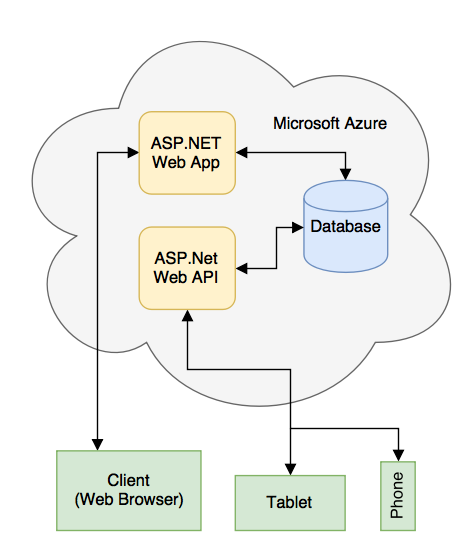
\includegraphics[width=0.65\textwidth]{./DesignImages/OverallDataFlowChp1.png}
\end{center}
\caption{System Diagram \label{systemdiagram}}
\end{figure}

\section{Technologies Overview}
\subsection{System Technology}
\begin{itemize}
\item \href{https://www.visualstudio.com/}{Microsoft Visual Studio} is used for web API, web application, and database code editing.
\item \href{https://azure.microsoft.com/en-us/}{Microsoft Azure} is used for hosting and maintaining the database, web API, and web application.
\item \href{http://square.github.io/retrofit/}{Retrofit} will be the framework used to handle RESTful HTTP requests.
\item \href{https://developer.android.com/studio/index.html}{Android Studio} will be used for the tablet application
\item A \href{http://www.samsung.com/us/mobile/tablets/all-other-tablets/samsung-galaxy-tab-a-8-0-16gb-wi-fi-smoky-titanium-sm-t350nzaaxar/}{Samsung Galaxy Tab} will be used for the tablet hardware.
\end{itemize}

\subsection{Documentation Technology}
\begin{itemize}
\item \LaTeX\ is used to generate this document.
\item \TeX\ maker is an editor used to edit the \LaTeX\ code.
\end{itemize}



%This section should contain a list of specific technologies used to
%develop the system.  The list should contain the name of the
%technology, brief description, link to reference material for further
%understanding, and briefly how/where/why it was used in the %system.
%See Table~\ref{somenumbers}.  This is a floating table environment.


%\begin{table}[tbh]
%\caption{A sample Table ... some numbers. \label{somenumbers}}
%\begin{center}
%\begin{tabular}{|r|l|}
%  \hline
%  7C0 & hexadecimal \\
%  3700 & octal \\ \cline{2-2}
%  11111000000 & binary \\
%  \hline \hline
%  1984 & decimal \\
%  \hline
%\end{tabular}
%\end{center}
%\end{table}

  %% All tracks
'% !TEX root = DesignDocument.tex

\chapter{User Stories,  Requirements, and Product Backlog}
\section{Overview}


The following section of this documentation describes the user stories provided, the requirements, and the product backlog. The user stories are provided by Dr. Jeff McGough, Dr. Christer Karlsson, and Mr. Brian Butterfield. From these user stories we have compiled a list of requirements and a product backlog.\footnote{See Appendix \ref{FutureAppendix}} 

\section{User Stories}
The given user stories are listed below:

\subsection{User Story \#1}
As a professor, I would like to display my weekly schedule.  
\subsubsection{User Story \#1 Breakdown}
It would be beneficial to show this schedule so students can know when I am available for office hours.  This would reduce the many emails and interruptions while I am working.  It also allows for easier access to my free time, giving the student a more chance to meet with me.

\subsection{User Story \#2} 
As a professor, I would like to permanently update my schedule with ease.  
\subsubsection{User Story \#2 Breakdown}
It is a nuisance to re-print a paper schedule every time it updates.  I would like to be able to update a change to my schedule within a matter of seconds.

\subsection{User Story \#3} 
As a professor, I would like to display a message.  
\subsubsection{User Story \#3 Breakdown}
It would be helpful to send important and quick messages for everyone to see. This increases the level of communication between faculty and student.

\subsection{User Story \#4} 
As a professor, I would like to display a message that directly affects my schedule, therefore, also temporarily updates my schedule. 
\subsubsection{User Story \#4 Breakdown}
Many things happen which could cancel or modify an event such as a snow day, sick day, or an important meeting.  It is important to keep the students informed as to what is happening with class and office hours.

\subsection{User Story \#5} 
As the office personnel, I would like to display a current or ongoing event in each classroom/lab. 
\subsubsection{User Story \#5 Breakdown}
Displaying a classroom schedule makes it easier for students and faculty to find open classrooms for meetings and events.

\subsection{User Story \#6} 
As the office personnel, I would like to display each classroom/lab's schedule. 
\subsubsection{User Story \#6 Breakdown}
Displaying a classroom schedule makes it easier for students and faculty to find open classrooms for meetings and events.

\subsection{User Story \#7} 
As the office personnel, I would like to display messages for certain rooms.
\subsubsection{User Story \#7 Breakdown}
The ability to quickly post a message on a room would reduce the confusion and hassle when a class is canceled or changed.  It would be way faster than printing a message to manually post on the door.

\subsection{User Story \#8} 
As the office personnel, I would like to receive and answer request for reservations on rooms. 
\subsubsection{User Story \#8 Breakdown}
There are a multitude of events happening throughout the semester at a college campus.  It would be helpful to make the process easier for scheduling all these events.

\subsection{User Story \#9} 
As a professor or office personnel, I would like the ability to send out push notifications. 
\subsubsection{User Story \#9 Breakdown}
A mobile update would most likely reach a student faster than email, so a push notification would be a more efficient way to get information to the students. 

\subsection{User Story \#10} 
As a student, I would like to request a reservation for a room.  
\subsubsection{User Story \#10 Breakdown}
Students have many group projects that require work at school outside of class.  It would help to have a room reserved, so the students don't have to wander around campus in order to find a classroom that appears to be empty.

\subsection{User Story \#11} 
As a student, I would like to receive push notifications.
\subsubsection{User Story \#11 Breakdown}
Receiving a push notification would most likely be a quicker way of getting information regarding classes. The faster the communication, the better.

\subsection{User Story \#12} 
As a student, I would like to know if the professor is inside his/her office and is available.  
\subsubsection{User Story \#12 Breakdown}
Students often need help with homework, advice and feedback from their instructors.  A more accurate schedule for the instructor lessens the time wasted trying to contact the instructor.

\subsection{User Story \#13} 
As a user, I would like the system to be very secure.  It is important to not have my personal information in the hands of anyone else.
\subsubsection{User Story \#13 Breakdown}
In order to have a secure system the following items must be addressed:
\begin{itemize}
\item Unauthorized database access
\item Hardware on the door is in lockdown mode
\item Verification for individual users
\end{itemize}

\subsection{User Story \#14} 
As a user, I would like to be able to log in to the system and be a distinguished user.  Again, security is very important.  I do not want my personal schedule and password in the hands of anyone other than those with the authorized role to view it.
\subsubsection{User Story \#14 Breakdown}
After a user logs in, the system displays the correct data and forms.

\section{Requirements and Design Constraints}
Listed below are details on the requirements and design constraints for this project.


\subsection{System  Requirements}
\begin{itemize}
\item The tablet application will run on an Android based tablet.
\item The web application is accessible through any web browser.
\end{itemize}

\noindent A possible alternative to this system would be to run the tablet application on an ODroid environment. This Odroid environment involves an ODroid, a display screen, a wifi module, an eMMC module, usb camera, and a microSD card.


\subsection{Network Requirements}
In order to use this product, the user must have a connection to the internet. Also any educational institution considering purchasing this product should expect an increase in wi-fi traffic, determined by how many tablets will be installed. 


\subsection{Development Environment Requirements}
The web API and the web application are developed using Microsoft Visual Studio. The tablet application was initially required to be written using Xamarin forms, and, therefore, would have been cross-platform. With the change in requirements, Xamarin will no longer be used and the tablet application will be written in Android native.  

\subsection{Project  Management Methodology}
Both our client meetings and team meetings take place weekly. During the first semester of this course the client meeting was set for Wednesday at one o'clock p.m., and for the second semester client meetings were scheduled on Thursday at ten o'clock a.m. Both semesters had team meetings on Tuesday at seven o'clock p.m.


\section{Specifications}
The back-end of this product will be handled by Microsoft Azure. Microsoft Azure SQL Database uses Microsoft SQL Server to create, scale and extend the applications into the cloud. 

\section{Product Backlog}
\subsection*{Azure}
\begin{itemize}
\item Set up Azure
\item Create Azure database
\item User Authentication
\item App Communication
\end{itemize}

\subsection*{Web Application}
\begin{itemize}
\item Create Web App project
\item Upload Web App project to Azure
\item Create website login screen
\item Communicate with Azure
\item Create schedule templates
\item \#30 Web App - Open calendar framework JSON events
\item \#31 Web App - Connect calendar event creation to database
\item \#33 Web App - Load events from database when navigating to dashboard controller
\item \#35 Create Unit test projects for both the web applications and web API projects
\item \#37 Web App (TEAM) - Create wireframe for design
\item Code the user interface according to wireframes
\item \#58 Web App - Add code to insert calendar events into database
\item \#59 Web App - Grab JSON from calendar framework
\item \#60 Web App - Load events from database
\item Create distinguished views for each type of user
\item Role based detection
\item Registration process
\item Database table integration and referencing
\item Repetition to generate repeated calendar events
\item Handle temporary canceled events
\end{itemize}

\subsection*{Web API}
\begin{itemize}
\item Create Web API project
\item Update Web API project to Azure
\item Model Location
\item Repository Layer
\item Serialize data
\item Migration on database
\item Create API endpoints for moving schedule data back and forth
\item \#24 Web API - Create Professor Model
\item \#25 Web API - Create Office Personnel Model
\item \#26 Web API - Create Calendar Event Model
\item \#27 Web API - Model Location
\item \#28 Web API - Create GetCalendarEvent endpoint
\item \#29 Web API - Create GetCalendarEvents endpoint
\item \#32 Web API - Create SaveCalendarEvents endpoint
\item \#35 Create Unit test projects for both the web applications and web API projects
\item \#41 Web API - Repository Layer
\item \#43 Web API - Serialize data
\item \#61 Web API - Fix Models
\item \#62 Web API - Create GetCalendarEventsByOwner endpoint
\item \#64 Web API - Create GetCalendarEventsByRoom
\item \#67 Web API - Display options endpoints
\item \#68 Web API - Create GetCalendarEventsByRange
\item \#69 Web API - Model updates
\item Testing
\end{itemize}

\subsection*{Tablet Application}
\begin{itemize}
\item Design and create splash screen
\item Enable tablet to connect to Azure
\item Create communication class
\item Display a message on tablet screen
\item Display schedule on tablet	
\item Learn Xamarin\footnote{See Appendix \ref{XamarinAppendix}\label{note1}}
\item Create Xamarin tablet application with a login page\textsuperscript{\ref{note1}}
\item \#18 Tablet App - Android Kiosk Mode for Tablet App
\item \#36 Tablet App - Create Calendar View
\item \#38 Tablet App (TEAM) - Create wireframe for tablet app
\item Code the user interface according to wireframes
\item \#39 Tablet App - Create communications class
\item \#40 Tablet App - Create a way to display JSON calendar events
\item \#42 Tablet App - Move Tablet Code
\item \#53 Android calendar framework JSON function
\item Create pop-up window with description
\item Modify week view class open source
\item Added synchronization button
\item Implement continuous synchronization
\item Create login page
\item Add a view to select calendar based on faculty or room
\item Token authentication
\item GUI modifications
\item Handle temporary canceled events
\item Testing
\end{itemize}

\subsection*{Miscellaneous}
\begin{itemize}
\item Logo
\item Research Tablet vs Odroid Options
\item Connect Visual Studio to Azure
\item Look into networking for tablets
\item Look into a pre-built calendar framework for displaying calendar events
\item Create middleman project
\item Make sure system is very secure
\item \#54 Understand how event ownership works
\end{itemize}

%\section{Research or Proof of Concept Results}
%This section is reserved for the discussion centered on any research that needed 
%to take place before full system design.  The research efforts may have led to 
%the need to actually provide a proof of concept for approval by the stakeholders. 
% The proof of concept might even go to the extent of a user interface design or 
%mock-ups. 



  %% All tracks (minimal for research track)
% !TEX root = DesignDocument.tex

\chapter{Project Management}

\section{Team Member's Roles}
The team members for this project are Andrew Fagrey, Jayson Kjenstad, and Samantha Kranstz. The team members were selected by the Senior Design course instructor, Dr. McGough. All team members serve as developers and testers for each part of this project. The respective roles for each project are as follows:

\begin{itemize}
\item Andrew Fagrey acted as a type of scrum master as well as a developer on the project focusing mainly on the web application development.
\item Samantha Kranstz served as a developer on the project focusing mainly on the web API development.
\item Jayson Kjenstad served as a developer on the project focusing mainly on the tablet application development.
\end{itemize}

\section{Project  Management Approach}
We will be developing our project using the Agile development methodology. This will allow the team flexibility as we develop the product over the course of two semesters. Each sprint will be approximately two and a half weeks long. The project source code, product backlog, and documentation are hosted in a Bitbucket repository owned by Dr. McGough. The user stories, sprint milestones, and sprint issues are also managed in Bitbucket. The team makes use of the Bitbucket wiki pages that allow the team to post questions and have discussions about various aspects of the project.

\section{Stakeholder Information}
The stakeholders for this project include Dr. McGough, Dr. Karlsson, and Brian Butterfield. The team members are also stakeholders for the project. Future users of the product could also be considered stakeholders for the project if the development of the project continues after this senior design course.

\subsection{Customer or End User (Product Owner)}
The end users for this product will primarily be educational institutions. Professors and office personnel in educational institutions will be able to make use of the tablet application and web application, whereas students could make use of an accompanying student mobile application.

\subsection{Management or Instructor (Scrum Master)}
Andrew Fagrey acts as a mini scrum master for this project by helping to break up the work for each sprint and solve team development obstacles. Dr. Karlsson helps to manage the overall project, and Brian Butterfield helps with overall design and architecture of the project. 

\subsection{Investors}
There are currently no financial investors for this project. This could change if development continues after the Senior Design course.

\subsection{Developers and Testers}
The main developers for this project are Andrew Fagrey, Samantha Kranstz, and Jayson Kjenstad. All developers for this project will also be testers. Every developer who writes code will be responsible for writing the accompanying tests for that code. The project manager for this project is Dr. Karlsson. Brian Butterfield is the chief architect for this project.

\section{Budget}
This project doesn't really have a specific budget. None of the developers are receiving any financial compensation for working on this project. All of the tools that are being used in the development of the project are downloaded free of charge.\\

\noindent Microsoft Visual Studio Enterprise Edition and Microsoft Azure are being used free of charge due to 
educational discounts for each. Dr. Karlsson purchased a Samsung Galaxy Tablet for the team to use in the development of the tablet application. The purchase of the Samsung tablet has been the only cost to the team besides tuition.

\section{Intellectual Property and Licensing}
The South Dakota School of Mines and Technology and the South Dakota Board of Regents have intellectual property rights over this project.

\section{Sprint  Overview}
The DoorPanes project will be implemented in phases. They are as follows:

\subsection{User Stories and Requirements Gathering}
This phase will be used to collect all user stories, requirements, limitations, and specifications for the project from the respective clients. The software contract between the clients and the developers will be written and signed during this phase of the development as well.

\subsection{Researching and Designing}
During this phase, we will be researching our options for the design, software, and hardware that could be used in the development of the project. After exploring these options, we will be deciding on the best course of action to take in the development of the project.

\subsection{Application Development}
All application development will occur during this phase of the project. The implementation of this project will follow all of the client's requirements gathered in the earlier phases in the project.

\subsection{Prototype Development}
The result of our developmental efforts will be a prototype of the project. The prototype will be a basic proof of concept. It will not be a full-fledged example of how the product will work, but just enough of an implementation to showcase the possibilities if the project were completed. The prototype for the project will include a responsive web application, a web API with a few calendar event endpoints, and a tablet application. 

\subsection{Testing Phase}
After the initial development of the project, we will spend some time thoroughly testing the code that we have developed for the project and the prototypes.

\subsection{Delivery}
The final phase of the project will be the delivery of the product. This product includes several components: the web application, the web API, and the tablet application. 

\section{Terminology and Acronyms}
Below is a list of terms and acronyms that will be used throughout this design document to describe the various parts of the DoorPanes project.

\begin{itemize}
\item MVC - Model View Controller
\item VS - Microsoft Visual Studio
\item API - Application Programming Interface
\end{itemize}

\section{Sprint Schedule}
The sprint schedule is listed below. The sprint schedule was largely determined by the Senior Design course instructor.

\begin{itemize}
\item Sprint 1: 9/12/16 - 10/1/16
\item Sprint 2: 10/10/16 - 10/29/16
\item Sprint 3: 11/7/16 - 11/26/16
\item Sprint 4: 1/9/17 - 1/27/16
\item Sprint 5: 2/6/17 - 2/24/17
\item Sprint 6: 3/13/17 - 4/6/17
\item Design Fair: 4/25/17
\end{itemize}

\section{Timeline}
\begin{figure}[tbh]
\begin{center}
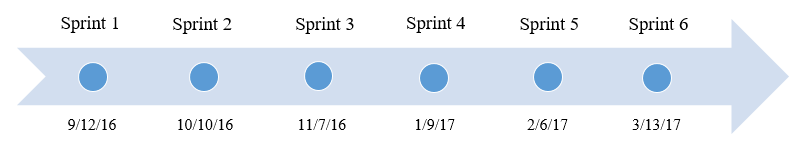
\includegraphics[width=0.75\textwidth]{./timeline.PNG}
\end{center}
\label{sprinttimeline}
\end{figure}

\section{Backlogs}

\subsection*{Sprint 1}
\begin{itemize}
	\item Set up Azure
	\item Create Azure database
	\item Create Azure app service
	\item Research Tablet vs Odroid Options
	\item Learn Xamarin\footnote{See Appendix \ref{XamarinAppendix} \label{note10}}
\end{itemize}

\subsection*{Sprint 2}
\begin{itemize}
\item Create Web App project
\item Upload Web App project to Azure
\item Create Web API project
\item Update Web API project to Azure
\item Create Xamarin tablet application with a login page\textsuperscript{\ref{note10}}
\item Create API endpoints for moving schedule data back and forth
\end{itemize}

\subsection*{Sprint 3}
\begin{itemize}
\item \#18 Tablet App - Android Kiosk Mode for Tablet App
\item \#24 Web API - Create Professor Model
\item \#25 Web API - Create Office Personnel Model
\item \#26 Web API - Create Calendar Event Model
\item \#27 Web API - Model Location
\item \#28 Web API - Create GetCalendarEvent endpoint
\item \#29 Web API - Create GetCalendarEvents endpoint
\item \#30 Web App - Open calendar framework JSON events
\item \#31 Web App - Connect calendar event creation to database
\item \#32 Web API - Create SaveCalendarEvents endpoint
\item \#33 Web App - Load events from database when navigating to dashboard controller
\item \#35 Create Unit test projects for both the web applications and web API projects
\item \#36 Tablet App - Create Calendar View
\item \#37 Web App (TEAM) - Create wireframe for design
\item \#38 Tablet App (TEAM) - Create wireframe for tablet app
\item \#39 Tablet App - Create communications class
\item \#40 Tablet App - Create a way to display JSON calendar events
\item \#41 Web API - Repository Layer
\item \#42 Tablet App - Move Tablet Code
\item \#43 Web API - Serialize data
\end{itemize}

\subsection*{Sprint 4}
\begin{itemize}
\item Create middleman project
\item \#53 Android calendar framework JSON function
\item \#54 Understand how event ownership works
\end{itemize}

\subsection*{Sprint 5}
\begin{itemize}
\item \#58 Web App - Add code to insert calendar events into database
\item \#59 Web App - Grab JSON from calendar framework
\item \#60 Web App - Load events from database
\item \#61 Web API - Fix Models
\item \#62 Web API - Create GetCalendarEventsByOwner endpoint
\item \#64 Web API - Create GetCalendarEventsByRoom
\item Tablet App - Create pop-up window with description
\item Tablet App - Modify week view class open source
\item Tablet App - Added synchronization button
\item Tablet App - Implement continuous synchronization
\item Tablet App - Create login page
\item Testing
\end{itemize}

\subsection*{Sprint 6}
\begin{itemize}
\item \#66 Web App - Add Authorization code
\item \#67 Web API - Display options endpoints
\item \#68 Web API - Create GetCalendarEventsByRange
\item \#69 Web API - Model updates
\item Web App - Create distinguished views for each type of user
\item Web App - Role based detection
\item Web App - Registration process
\item Web App - Database table integration and referencing
\item Web App - Repetition to generate repeated calendar events
\item Web App - Handle temporary canceled events
\item Tablet App - Add a view to select calendar based on faculty or room
\item Tablet App - Token authentication
\item Tablet App - GUI modifications
\item Tablet App - Handle temporary canceled events
\item Testing
\end{itemize}

\section{Burndown Charts}
\begin{figure}[tbh]
\begin{center}
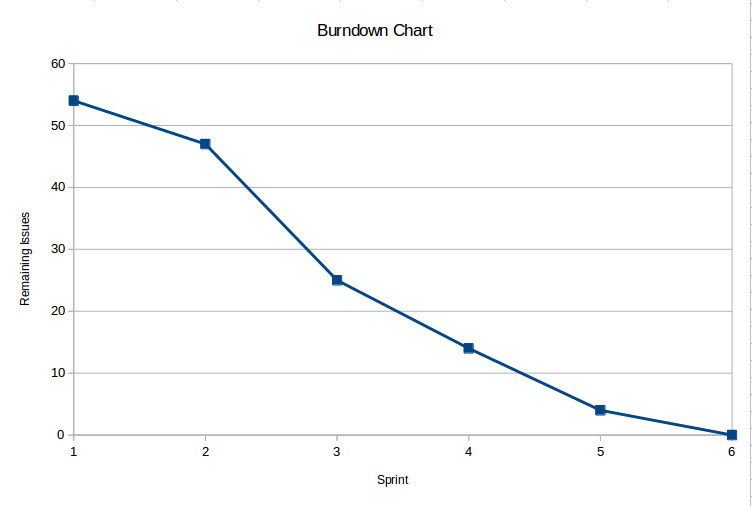
\includegraphics[width=0.75\textwidth]{./Burndown.png}
\end{center}
\label{BurndownChart}
\end{figure}

\section{Development Environment}
To setup a machine for development towards this project, the developer must ensure that his development machine meets the list of requirements shown below. Development machines must have:

\begin{itemize}
\item Windows 10 or later running on the machine.
\item Microsoft Visual Studio Enterprise Edition installed.
\item Android Studio installed.
\item Android SDK with a minimum API level of 23 installed.
\end{itemize}

\noindent The project files and code for the web application and web API must be downloaded from the Bitbucket repository. The web application and web API projects (as well as the testing projects for each) are contained in a Visual Studio Solution. Opening up the Visual Studio solution file should open the web application and web API projects, along with their respective testing projects.\\ 

\noindent The Android Studio solution is contained in a separate repository. The solution can be downloaded from the repository, and then it can be opened, built, and run in Android Studio.

\section{Development IDE and Tools}
Each team member is using their SDSM\&T Tablet PC running Microsoft Windows 10 for the development of this project. The team is using Microsoft Visual Studio Enterprise Edition as an IDE for this project for the web application and the web API. Microsoft Azure is being used as the back-end for this project. The Android tablet app is being developed with Android Studio and the Android SDK. We also are using a Samsung Galaxy Tab A8 for the tablet application development.

\section{Source  Control}
Bitbucket is used for code versioning and management. Dr. McGough created a repository and added each team member to the repository. All team members have write access. A second repository was created to host the tablet application source code. A developer can connect to the repository by responding to an invite from an administrator of the repository.

\section{Dependencies}
The web application and web API projects are dependent on the Microsoft ASP.NET platform, whereas the Android application will be depended on the Android SDK.

\section{Build  Environment}
The web application and web API projects are built and run in Visual Studio. The testing projects for the web application and web API are also built and run in Visual Studio. The Android application is built and run in Android Studio.

\section{Development Machine Setup}
A machine can be used for development on this project if it is capable of running Windows 10, Visual Studio, and Android Studio with the SDK. To setup your machine, follow the following steps:

\begin{itemize}
\item Make sure you are are running Windows 10. If not, you must either purchase Windows 10 and install it on your current machine, or upgrade to a machine capable of running Windows 10. 
\item Purchase and install Microsoft Visual Studio Enterprise Edition.
\item Download Android Studio.
\end{itemize}


   %% All tracks
% !TEX root = DesignDocument.tex

\chapter{Design  and Implementation}
In this section, we describe the design details for each of the major components in our product. In this chapter, we will discuss the architecture and system design for our product, which includes the design selection, a diagram of the data flow in our product, communication and classes in each of the projects, and mock up screen-shots of all the GUI interfaces that our product has now or will have later. In addition, each of the major components of the product are described in more detail below.
 

\section{Architecture and System Design}
Part of our project is hosted in the cloud by Microsoft Azure. It is here that our database, web application, as well as our API are hosted. The web application is used to create the calendar data and store it in the database. This web application is responsible for the creation of accounts, whether it be a student, professor, or other faculty member.  Once logged in, the web app can be used to create events for a faculty or room calendar.  When the calendar is created, all the events can be viewed and modified on the main dashboard screen.\\


The web API can be used to get the needed data from the database and show the calendar on the tablet application.  The API has a number of calls to get data for the tablet app based on certain parameters.  There is a login endpoint which will give a token based on correct authentication input.  There are also a number of endpoints used to return a list of events based on certain criteria such as room or faculty names.\\

The tablet application uses these API calls and displays the data accordingly.  As mentioned above, it first uses a token endpoint where it sends the inputted user name and password in a body to the API.  The response given back determines if the user is authenticated or not.  If successful, the user can access all other API get event calls while using this authentication token.

  

\subsection{Design Selection}
A majority of our design for this project was directly affected by our decision on hardware.  Our hardware options were between an Android tablet or an ODroid based setup. The ODroid environment included many parts: an ODroid, a display, a camera, a wifi adapter, and a few other parts. As for the Android tablet, we needed to figure out the best tablet that fit our project needs. So after some deliberation, we went with a Samsung Galaxy Tab 8A for our hardware.  This tablet was about the same cost as an ODroid system.  We determined it would be better to focus this product on software that is able to be used on any Android device.  The potential few dollars we would save on an ODroid was not worth the setup time to configure the whole device.\\

The next decision to be made was whether to write our code in an exclusive Android environment and code the iOS applications later, or write the code using Xamarin forms for cross platfom development. We decided to save time in the future by writing it using Xamarin now. So the tablet application and the mobile application are being written using Xamarin forms.

Edit: Starting in the Spring semester of Senior Design, we are no longer using Xamarin forms for the tablet application of this project.  All developent will be done in Android Studio..........

 
\subsection{Data Structures and Algorithms}
This program follows the dataflow shown in Figure ~\ref{overallDataflow}. This is in a sense our algorithm.  The data will be created using a webportal where the information is stored in the database.  From here we will use the API to grab the needed data and display it on the tablet.  The API will have calls allowing us to grab data such as daily events, professor infomation, special messages, etc.\\

For example, a user can create an account or log in to the web application. Once authenticated, he or she can create an event on the calendar by clicking where the event is to be started, dragging the mouse to the end time of the event.  A box will then come up wich allows the user to edit the name of the event, and manually adjust the times.  Once the user saves this event, it is stored in the database.  We now need a way for this data to be sent to out tablet application.  This is where the API is used.\\ 

A user can then log into the tablet application (Which needs the API as well), and select the calendar that was just edited in the web application.  When the user syncs the calendar, the tablet application uses a API get call to retrieve all events which match the selected calendar.  The API will go to the database, find all events which match the calendar in the call, and return a list of calendar events.  The tablet application can then parse this response, and use the data to display the events.
 
\subsection{Data Flow}
Below is a diagram that shows the data flow for this project. Each of the components shown in the diagram are described in Figure ~\ref{overallDataflow} in greater detail. The figure shows how the database, web API, and the web application connect together and pass data back and forth.The figure also shows how this data is passed to and from the tablet application.
 
\begin{figure}[h!]
\centering
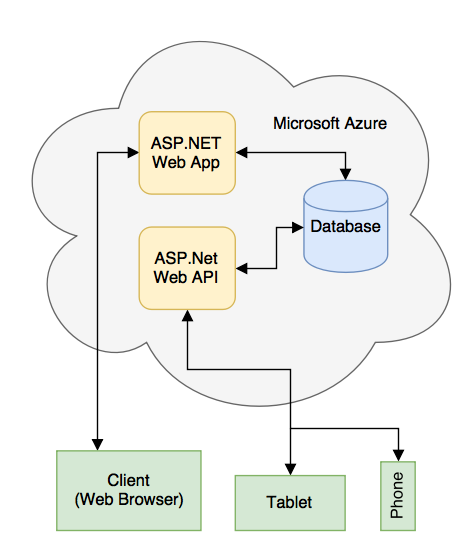
\includegraphics[scale=0.5]{DesignImages/OverallDataFlow.png}
\caption{Project Dataflow}
\label{overallDataflow}
\end{figure} 
 
\subsection{Communications}
One of the main communications in this project is between our RESTful API and the tablet application. A RESTful API uses HTTP requests to GET, POST, PUT, and DELETE. These requests return data in a JSON formatted string for the tablet to consume. The other communications in this project are the web app with the database and the web API and the database.\\

The HTTP client used for communication between the tablet application and the API is called Retrofit. It is a type safe HTTP REST client for Java. Retrofit provides a framework for interacting with API's and sending network requests with OKHTTP. There is also built in JSON parsing.  The JSON responses returned by the API calls can be parsed and filled into defined Java Objects.  
 
 
 
\subsection{Classes}
Here is a list of classes used by the web application and by the web API projects.
\begin{itemize}
\item Account Controller Class - Manages the accounts 
\item Calendar Controller Class - Manages the calendar events
\item Home Controller Class - Manages the main homepages
\item Calendar Event Repository Class - Implementation of the methods for calendar events
\item ICalendar Event Repository Class - Interface, lists methods for calendar events
\item University Context Class - Connects the models to the database
\item Account Binding Models Class - Used for handling accounts
\item Account View Models Class - Used for handling account views
\item Calendar Event Class - Model outline for the calendar events
\item Identity Models Class - Used for authenticating an identity
\item Instructor Class - Model outline for an instructor, inherits from person
\item Office Personnel Class - Model outline for an office personnel, inherits from person
\item Person Class - Model that contains and checks input for first and last name
\end{itemize}

\begin{figure}[h!]
\centering
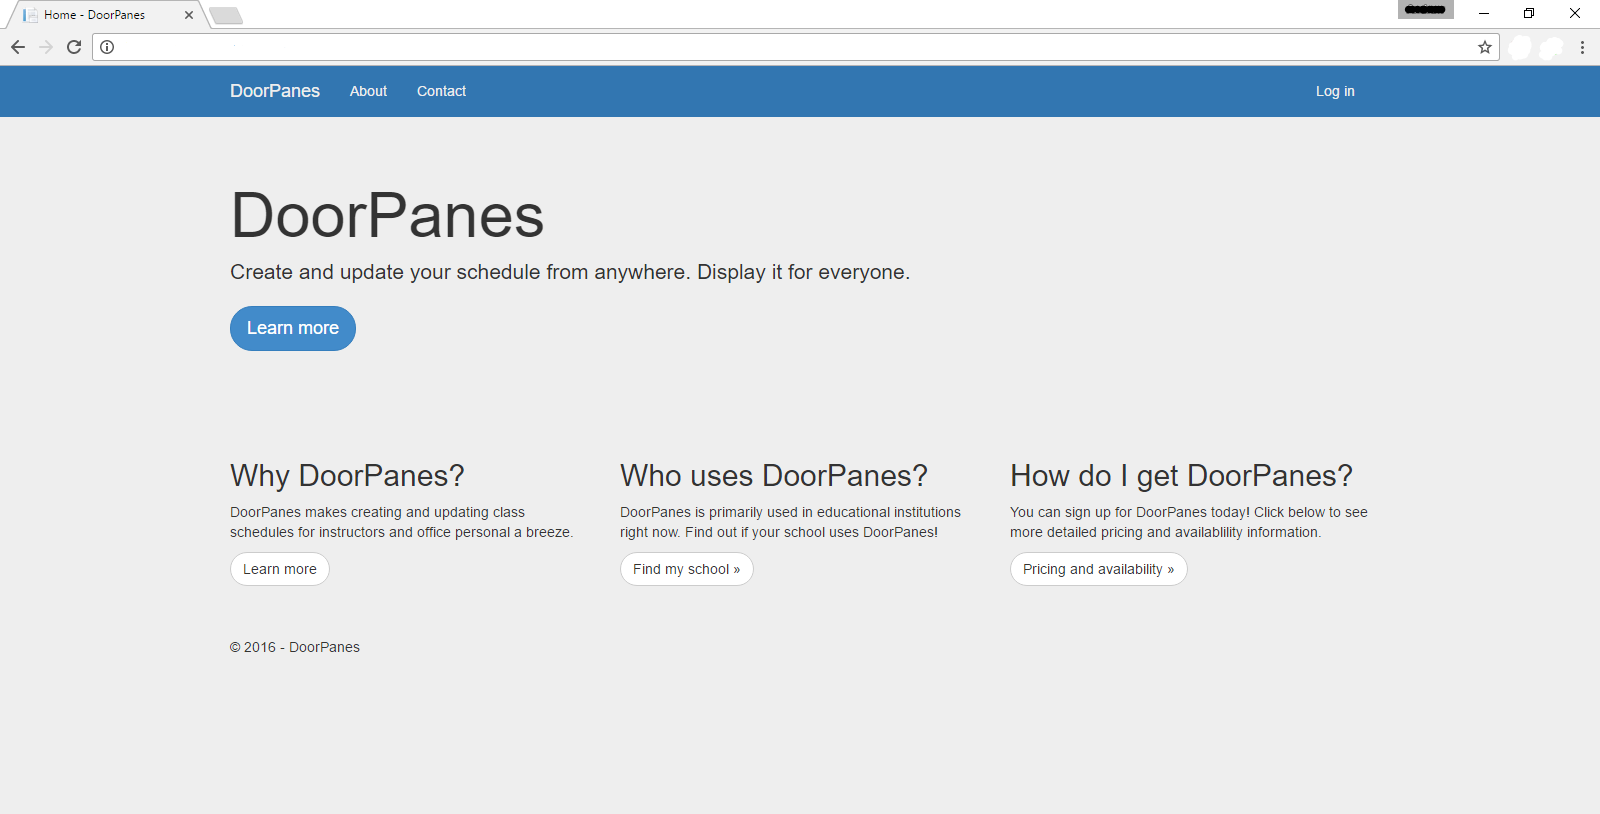
\includegraphics[scale=0.35]{DesignImages/DoorPanesWebAppHome.PNG}
\caption{Web Application Website Homepage}
\label{webAppHomePage}
\end{figure} 

\begin{figure}[h!]
\centering
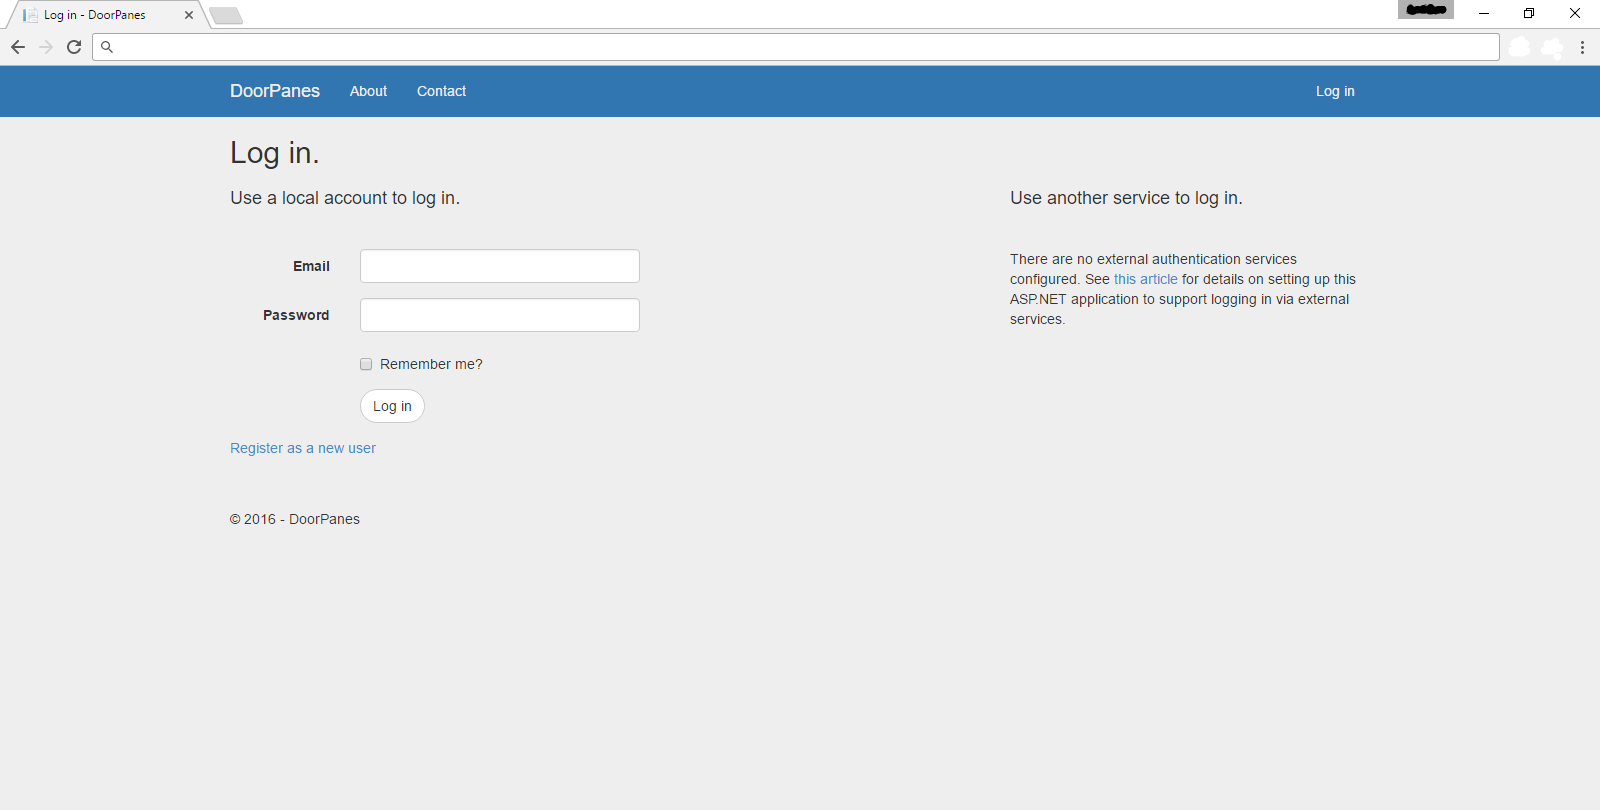
\includegraphics[scale=0.35]{DesignImages/DoorPanesWebAppLogin.PNG}
\caption{Web Application Login Page}
\label{webApplicationLoginPage}
\end{figure} 

\begin{figure}[h!]
\centering
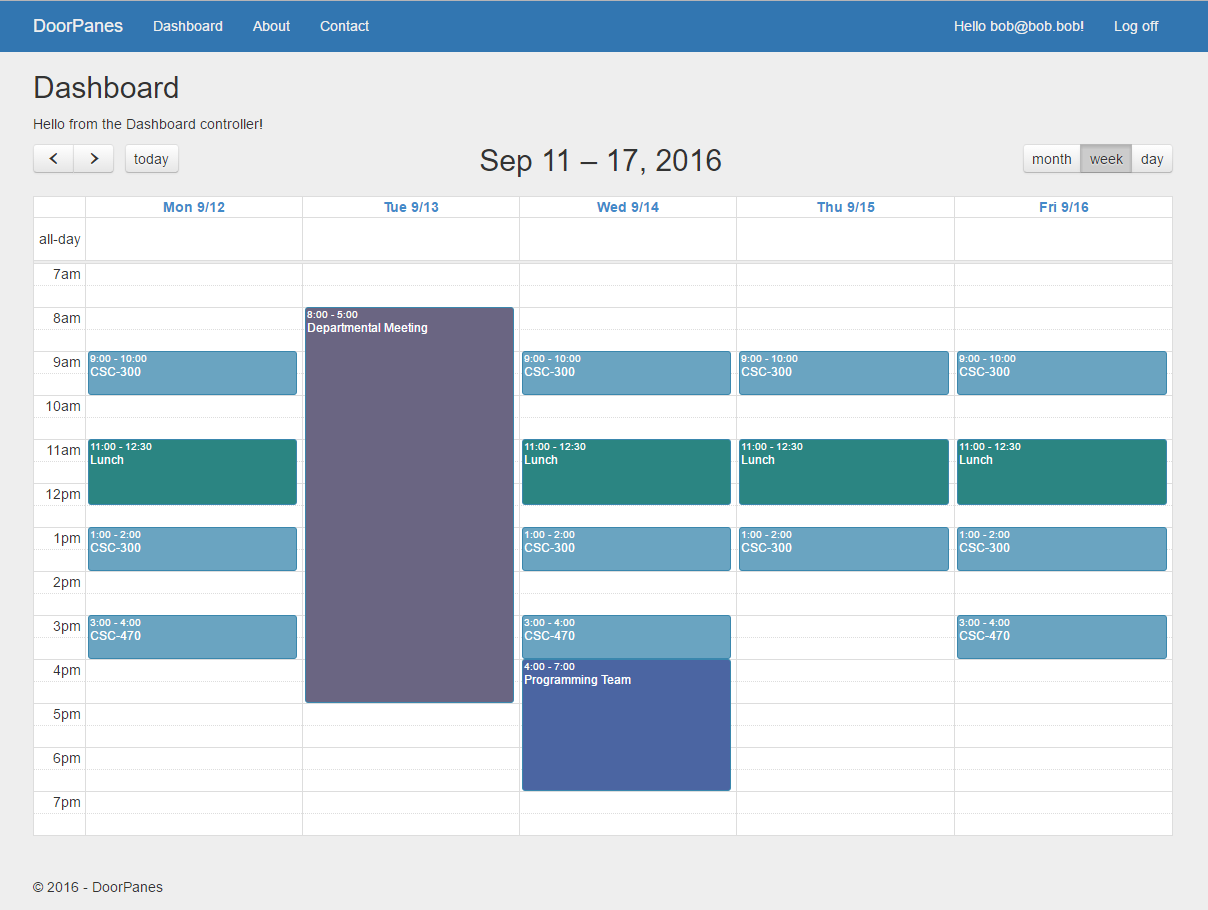
\includegraphics[scale=0.4]{DesignImages/DoorPanesWebAppCal.PNG}
\caption{Web Application Calendar Controller}
\label{webApplicationCalView}
\end{figure} 
 
\subsection{GUI}
Figure \ref{webAppHomePage}, Figure \ref{webApplicationLoginPage}, and Figure \ref{webApplicationCalView} are the application's current GUI screenshots:


Figure \ref{fig:login}, Figure \ref{fig:firstview}, Figure \ref{fig:selection}, Figure \ref{fig:dashboard}, Figure \ref{fig:finallogin}, and Figure \ref{fig:navdrawer} are the wireframe mockups of the user interfaces of the tablet application.  Figure \ref{fig:ScreenArchitecture} in section \ref{ArchitectureSection} shows how all of these screens connect.
 
\begin{figure}
\centering
  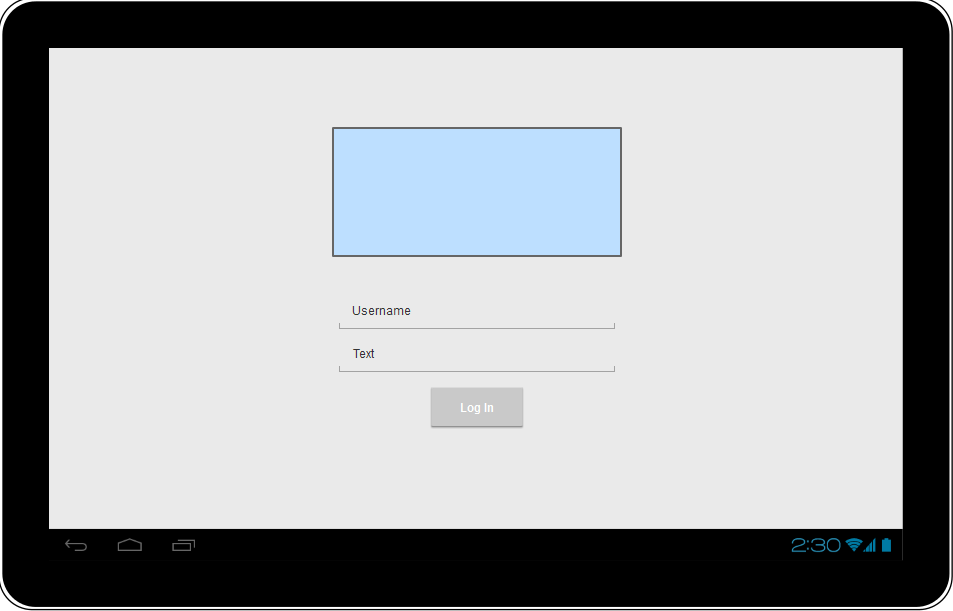
\includegraphics[scale=0.4]{login.png}
  \caption{Login page}
  \label{fig:login}
\end{figure}


\begin{figure}
\centering
  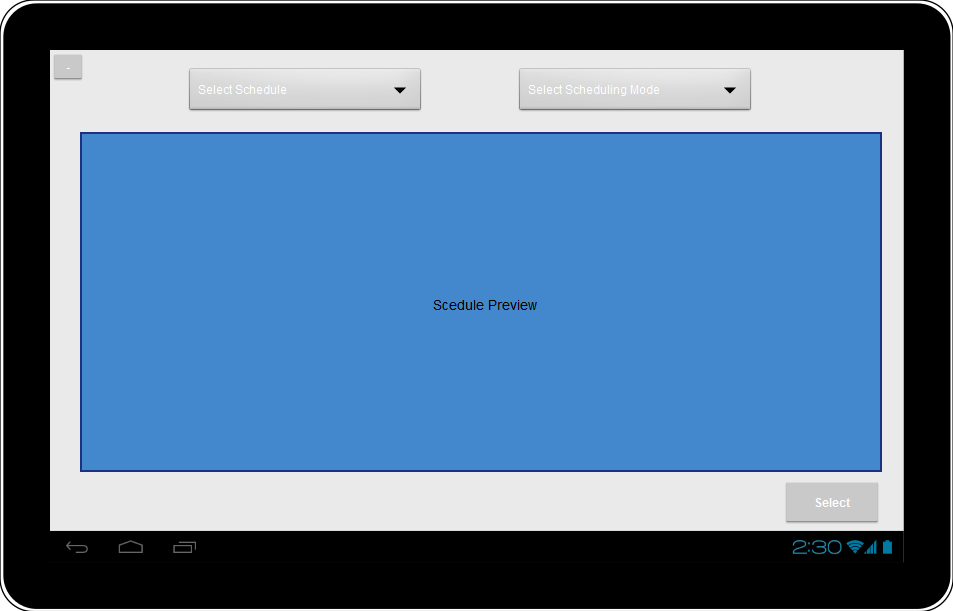
\includegraphics[scale=0.4]{firstview.png}
  \caption{Preview Page}
  \label{fig:firstview}
\end{figure}

\begin{figure}
\centering
  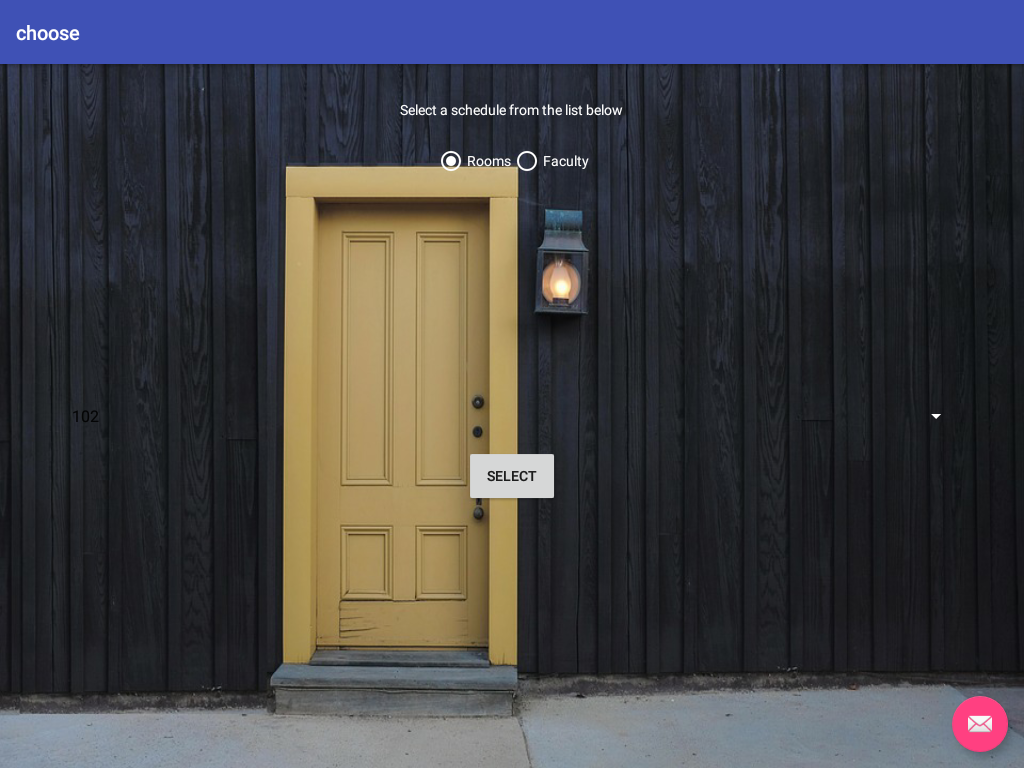
\includegraphics[scale=0.4]{selection_final.png}
  \caption{Preview Page}
  \label{fig:selection}
\end{figure}

\begin{figure}
\centering
  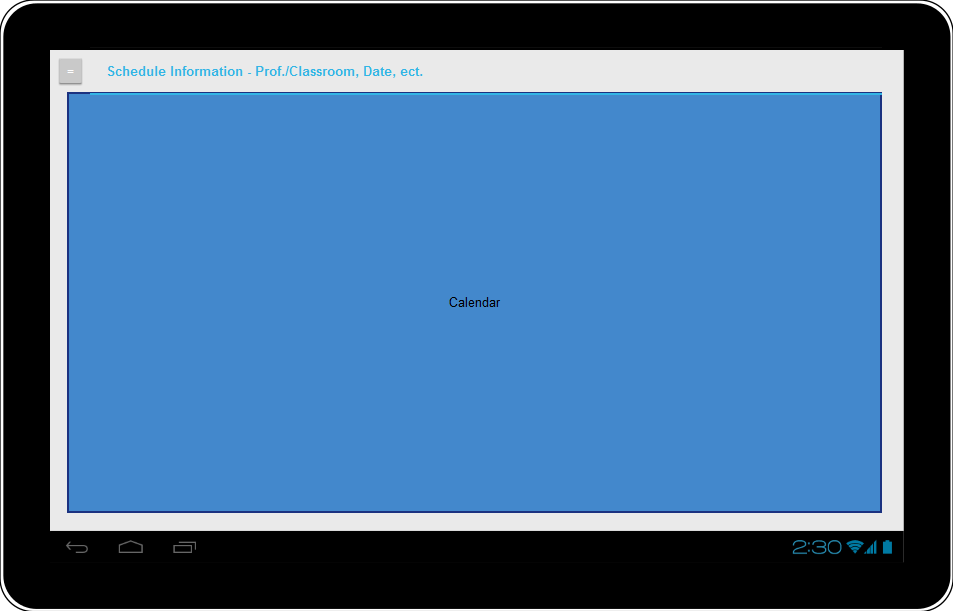
\includegraphics[scale=0.4]{dashboard.png}
  \caption{Dashboard view}
  \label{fig:dashboard}
\end{figure}

\begin{figure}
\centering
  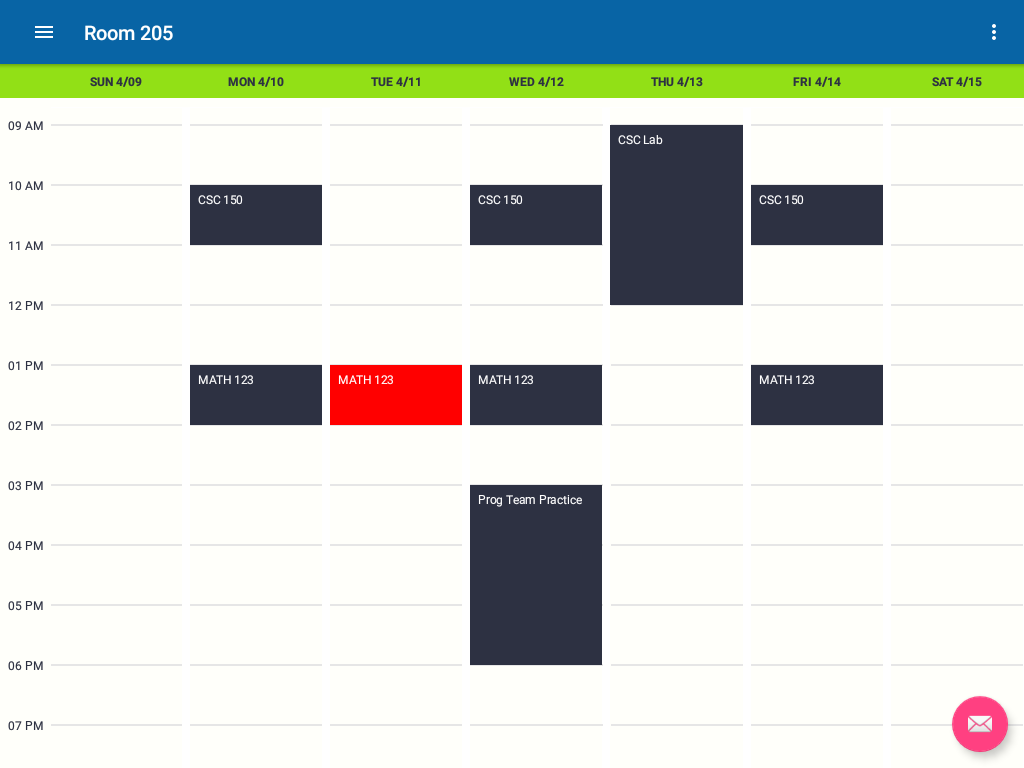
\includegraphics[scale=0.4]{dashboard_final.png}
  \caption{Login page}
  \label{fig:finallogin}
\end{figure}

\begin{figure}
\centering
  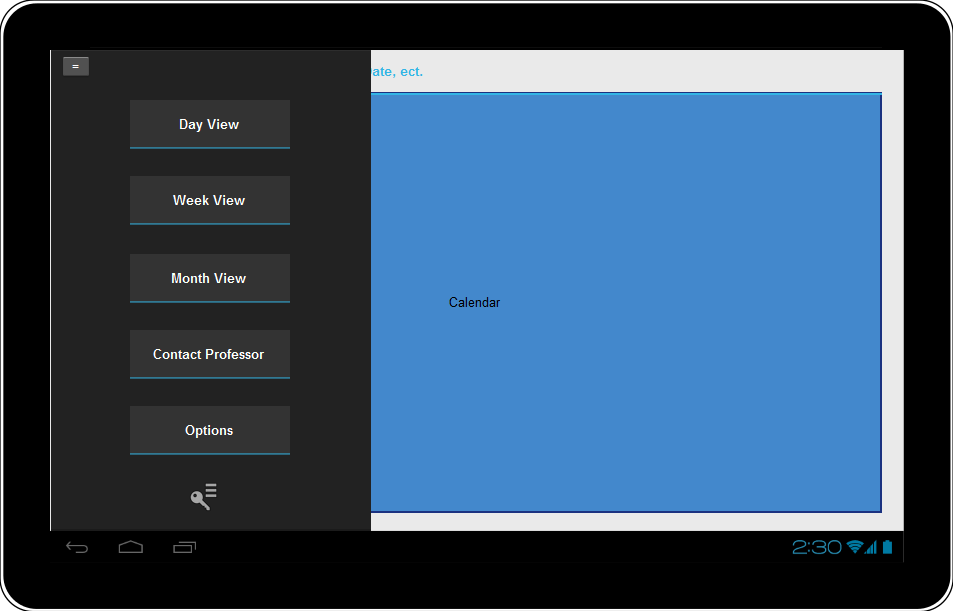
\includegraphics[scale=0.4]{navigationdrawer.png}
  \caption{Dashboard view with navigation drawer expanded}
  \label{fig:navdrawer}
\end{figure}

\begin{figure}
\centering
  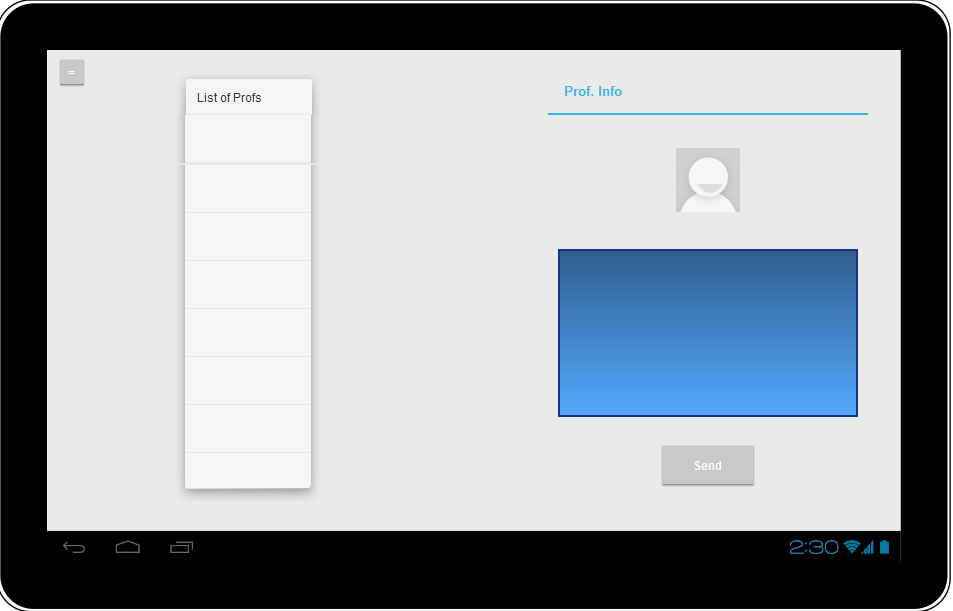
\includegraphics[scale=0.4]{contact.png}
  \caption{Contact Professor page}
  \label{fig:contactprof}
\end{figure}

\pagebreak
\section{Major Component \#1 - ASP.NET Web API}

\subsection{Technologies  Used}
\begin{itemize}
\item Microsoft Azure
\item Microsoft Visual Studio
\item Web Browsers
\item ASP.NET Razor markup
\end{itemize} 

\subsection{Component  Overview}
\begin{itemize}
\item Endpoints
\begin{itemize}
\item Login
\item Get Calendar Events
\item Get Calendar Events By Date
\item Get Calendar Events By Professor
\item Get Calendar Events By Room
\item Get A Calendar Event
\item Get A Instructor
\item Get Office Personnel
\item Add/Update/Delete Calendar Event
\item Add/Update/Delete Instructor
\item Add/Update/Delete Office Personnel
\item Add/Update/Delete Student
\end{itemize}
\item Models
\begin{itemize}
\item Instructor
\item Office Personnel
\item Student
\item Person
\item Calendar Event
\end{itemize}
\item Controllers
\begin{itemize}
\item Instructor
\item Office Personnel
\item Student
\item Calendar Event
\end{itemize}
\item Repositories
\begin{itemize}
\item Calendar Events Interface
\item Calendar Events
\item Instructor Interface
\item Instructor
\item Office Personnel Interface
\item Office Personnel 
\end{itemize}
\end{itemize}

\subsection{Phase Overview}
\begin{itemize}
\item Gathered User Stories
\item Researched and Designed
\item Process of Application Development
\end{itemize}

\pagebreak
\subsection{Dataflow Diagram}
\begin{figure}[tbh]
\begin{center}
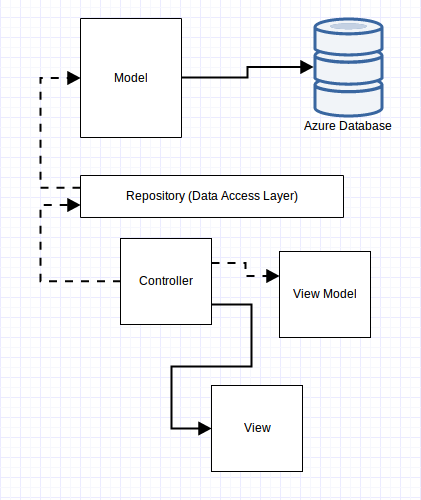
\includegraphics[scale=0.5,width=0.75\textwidth]{MVC5.png}
\caption{Web API Dataflow Diagram}
\end{center}
\label{APIMVC}
\end{figure}

\section{Major Component \#2 - ASP.NET Web App}

% This section was written by Andrew Fagrey

\subsection{Technologies  Used}
This section describes the various technologies used for the ASP.NET web application. Since the web application is hosted in Microsoft Azure, Azure handles most of the backend for keeping the web application up and running. The server that the web application is running on and the storage for the web application are all handled by Microsoft. In addition, Azure handles the publicly accessible URL for the web application. Here's a full list of the technologies we are currently using to support the web application:

\begin{itemize}
\item Microsoft ASP.NET Web App Framework
\item Microsoft MVC App Framework
\item Microsoft Azure Cloud Services
\item Microsoft Azure Database
\end{itemize}


\subsection{Component  Overview}
This section is a description of the various software components used in the web application. The web application is divided up into three main sections software-wise: the models, the views, and the controllers.\\

The web application models are classes that provide an abstraction and a representation of the data that is passed around in the web application. For example, the web application has a model for a calendar event, which contains fields pertaining to calendar details, like an event title, a start and end time, and an event owner.\\

The web application views contain the code that generates the HTML web pages that are viewed in a web browser. The view files are C\#-based files that make use of a Microsoft feature called Razor. Basically, Razor allows the C\# code to be intertwined with HTML code. This allows us to, for example, use C\# to generate an HTML list element without actually coding all the list tags ourselves.\\

The web application controllers are the classes that are used by the ASP.NET web application routing system to determine what code is run based on the URL given in a web browser. Each method inside the controller class corresponds to a different endpoint in the web application. As we develop the web application, we will have controllers for managing the various calender views, controllers for office personnel, and controllers for classrooms.\\

Below is a current list of the components that the web app either has or will have:


\begin{itemize}
\item A website homepage showcasing the product 
\item A login page accessible by a web browser
\item Calendar dashboard for viewing, creating, and editing calendar events
\item An open source calendar framework for displaying JavaScript-based events on the calendar framework
\item A website URL, which is currently www.doorpaneswebapp.azurewebsites.net
\item A convenient way to quickly cancel a set of events for a specific day
\end{itemize}


\subsection{Phase Overview}
This section describes the various development phases for the web application. This section is currently being updated as the development of the web application continues. Below is a list of development phases we went through as we developed the web application:

\begin{enumerate}
\item Gathered user stories for the web application
\item Built a test web application
\item Started to modify the web application to reflect the DoorPanes project
\item Published the web application on Microsoft Azure Cloud to start testing how it worked and what it looked like
\item Began developing and integrating calendar models and the open source calendar framework.
\item Currently working on expanding the model and controller list in conjunction with the web API.
\end{enumerate}


\subsection{Dataflow Diagram}
This section contains a dataflow diagram for the web application. The dataflow diagram shown in Figure ~\ref{webAppDataflow} shows how the data moves inside the web application.\\\\

\begin{figure}[h!]
\centering
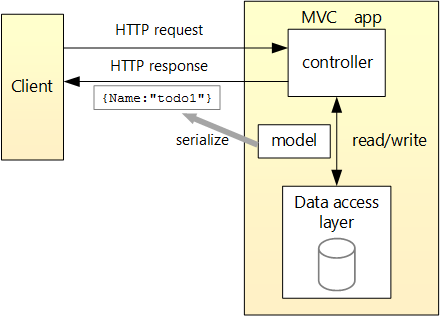
\includegraphics[scale=1.0]{DesignImages/webAppDataflow.png}
\caption{Web Application Dataflow Diagram. Image by Microsoft.}
\label{webAppDataflow}
\end{figure}

% CITE IMAGE
% https://docs.microsoft.com/en-us/aspnet/core/tutorials/first-web-api

\section{Major Component \#3 - Android Tablet Application}

\subsection{Technologies  Used}
To develop the tablet application for this project, Android Studio version 2.2.2 will be used. All testing for this project will be used on a Samsung Galaxy Tab 8A tablet running Android version 6.0 (Marshmallow) The target level for the execution of this application will be Android 6.0, API level 23. All testing done in Android will use Espresso testing framework.\\

In summary, here are the technologies used:

\begin{itemize}
\item Android Studio Version 2.2.2
\item Android SDK - target API level 23
\item Samsung Galaxy Tab 8A
\item Espresso Testing Framework
\end{itemize}



\subsection{Component  Overview}
The main goal of the tablet application is to display a schedule for a given classroom or professor. After logged in, a user can cycle through given schedules and look at different views: daily, weekly, and monthly.  There will also be a contact feature that will allow the user to send a message or email to a professor. \\

Here are the components that the tablet application will have when finished:

\begin{itemize}
\item A login page on application startup
\item A calendar preview/selection page
\item Dashboard view for viewing the chosen calendar
\end{itemize}

\subsection{Phase Overview}


Below is a list of the development phases of the tablet application:

\begin{itemize}
\item Gathered user stories
\item Set up Android environment
\item Created the login view
\item Created calendar select view
\item Created dashboard view
\item Create navigation menu 
\item Use API calls to get calendar information 
\item Create contact forms (pending)
\item Create different calendar views (pending)
\end{itemize} 


\subsection{ Architecture  Diagram}
\label{ArchitectureSection}
The architecture design for the tablet application is shown in Figure ~\ref{fig:Architecture}. The program will start on a login screen when open. If login is successful, a preview page will be shown. From this preview page, the user can select a schedule to be shown from a list of available schedules from the account. Once selected, the program goes to the dashboard view
\begin{figure}[h!]
  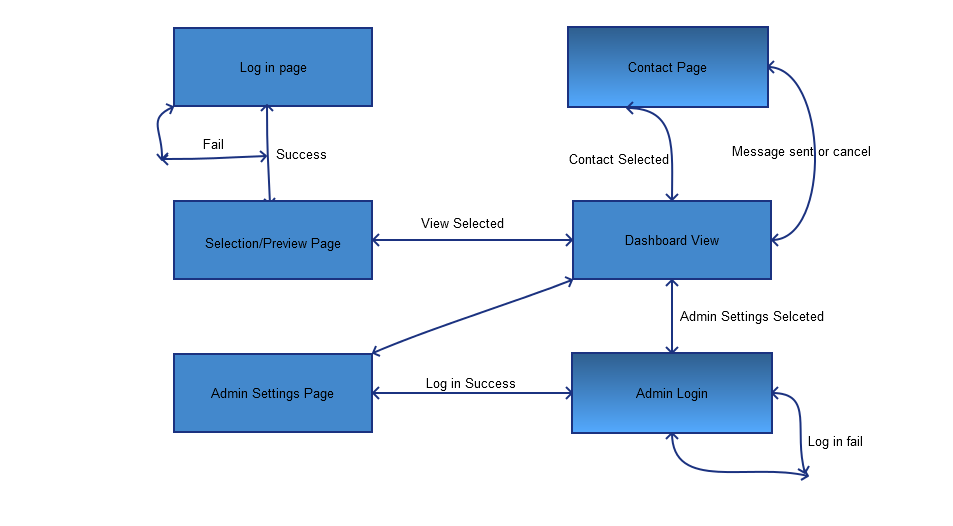
\includegraphics[width=\linewidth]{graph.png}
  \caption{Architecture Diagram}
  \label{fig:ScreenArchitecture}

\end{figure}
  %% All tracks
% !TEX root = DesignDocument.tex

\chapter{System  and Unit Testing}

\section{Overview}
This section describes the approach we are taking with regards to system and unit testing. This section provides a brief overview of our testing approach, the testing frameworks we will use, and a description of how the testing will be done to ensure that our system will be successful.

Most of the testing for this project was done in Sprint 5

\section{Dependencies}
The testing dependencies for our project components are as followed:
\begin{itemize}
\item Web application - Microsoft Visual Studio Testing Framework
\item Web API - Microsoft Visual Studio Test Explorer
\item Tablet application - Espresso testing framework
\item Tablet application - JUnit
\end{itemize}


\section{Test Setup and Execution}

\subsection{Web Application Unit Testing}
The unit tests for the Web App project will be contained in a C\# project under the DoorPanes Visual Studio solution. The testing project will contain a testing class for every endpoint controller in the normal C\# project. Each testing class will contain methods that will test every endpoint method in the normal C\# project. The unit tests will be run in Microsoft Visual Studio. The dashboard controller contains the following endpoints that can be unit tested:

\begin{itemize}
\item Index Endpoint - Shows the main page of the dashboard controller. Will be unit tested under the conditions of being authorized, not authorized, and simple navigation to the controller.
\item Get Events Endpoint - Gets all endpoints from the database. 
\item Insert Event Endpoint - Saves events created on the Web App into the SQL database.
\item There are various other endpoints that the JavaScript code calls, but most of it just returns existing data.
\end{itemize}

\noindent ASP.NET MVC unit tests directly call methods of your MVC controllers. When a unit test calls an action method in a controller, you can validate that the correct view is returned (although you do not validate the HTML) and that view data is returned. You can also test whether a method correctly redirects to another controller or view.

\subsection{Web API Unit Testing}
Microsoft Visual Studio allows the user to create an accompanying test project when creating an API project.  The above section describing the general idea of how the web application was unit tested also applies to how the web API was unit tested. Also Moq was used to  mock repositories and databases for unit testing. The following endpoints in the web API that are unit tested:

\begin{itemize}
\item Login
\item Get Calendar Events
\item Get Calendar Events By Range and Owner
\item Get Calendar Events By Range and Room
\item Get Calendar Events By Owner
\item Get Calendar Events By Room
\item Get A Calendar Event
\item Get All Owners
\item Get All Rooms
\item Delete All Calendar Events
\end{itemize}

\subsection{Tablet Application Unit Testing}
All unit testing for the tablet application for this project will be done using the JUnit testing framework.  JUnit is a JAR file linked in at compile time under the package junit.framework. All unit tests will follow the format listed in the code shown.
\lstinputlisting[language=Java]{test.java}

Unit tests for the tablet application have been written to test the login function of the application.  These tests use the Espresso testing framework for Java/Android. This is an automated UI testing framework.  The tests are written in a test file and when run, user input is emulated and run on the application.  You can see the user inputs specified in the test be displayed during the run of the test.  Every thought of input for the login screen will be inputted to make sure the application handles the errors correctly.  Invalid usernames and passwords are checked to make sure that a correct message and prompt is displayed to the user.  On correct input, the test will check that the application moves to the correct activity.

As mentioned above, Espresso is a UI testing framework.  Because of this, all UI elements can be tested.  These include all buttons, menus, etc.  The testing framework can act as the user and "press" all the buttons and menus in the program.  The test will check to make sure the appropriate action is taken after each UI interaction	

\begin{figure}
  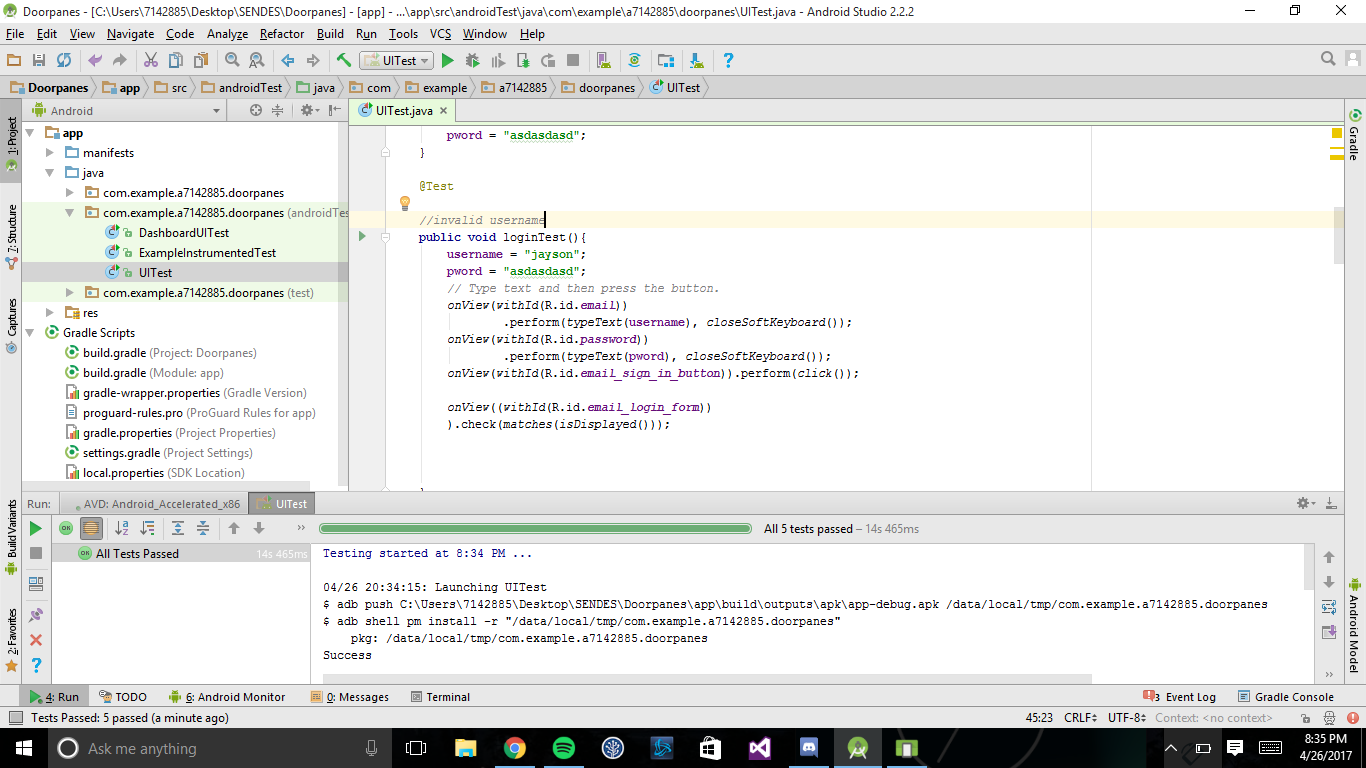
\includegraphics[width=\linewidth]{tablettest.png}
  \caption{Example of what a unit test looks like for the log in page.  You can see at the bottom of the page that all tests were successful!}
  \label{fig:tablettesting}
\end{figure} 

\section{System Testing}

One of the nice things about using Microsoft Azure is that performance testing, 	volume testing, stress testing, and scalability testing are all handled on the Microsoft Azure end. We don't have any control over the actual server hardware. All we would have to do is pay a higher price for more performance.\\

\noindent The following tests will be done to ensure the application is properly system tested.

\begin{itemize}
  \item GUI Testing - all parts of the interface will be tested to make sure the function and work properly.
  \item Usability testing - monitor how user uses the application and receive feedback based on there use of the program.
  \item Compatibility testing - make sure the application runs on all required versions of Android OS.
\end{itemize}

\section{System Integration Analysis}
For this project to work correctly, the tablet application needs to integrate the Web API calls.  API calls will be used to transfer data to and from the tablet application. To make sure all of these calls are working correctly and the system is properly integrated, tests will be written using JUnit, a Java testing framework.

\section{Risk Analysis}

\subsection{Web Application Risk Analysis}
There are no known risks that are under our control for the web application at this time.
\subsubsection{Risk Mitigation}
In terms of system risk analysis, we are  dependent on Microsoft for this. Hopefully Microsoft does a good job safeguarding the entrances to their data-centers and such.\\\\
\noindent
Possible risks for the web app include the risk of someone knowing a person's schedule. This could potentially increase the danger towards a person's safety. 

\subsection{Web API Risk Analysis}
The Web API for our project brings a few risks to consider, including the risk of SQL injections and other forms of accessing the database without permission.

\subsubsection{Risk Mitigation}
Taking these risks into account we will need to make the necessary steps to ensure that no unauthorized access is permitted.

\subsection{Tablet Application Risk Analysis}
The biggest issue in the tablet application will be security.  Our application needs to correctly identify and authenticate a user, and only they or users with access to that data can view and modify it.  The tablet application uses token based authentication.  A username and password is sent in a POST request.  If valid, a token will be returned which allows a user to access all the secure API calls.



\subsubsection{Risk Mitigation}
Care needs to be taken here. As of this moment, passwords and usernames may be sent in plain text.  HTTPS needs to be put into affect on this project to ensure no passwords can be watched over the network.

\section{Successes, Issues and Problems}

This section describes our successes and failure when it comes to the testing part of the project.

% Section Author: Andrew Fagrey
\subsection{Web Application}
When tested, the Web application had the following successes, issues, and problems:\\\\
\subsubsection{Successes}
\begin{itemize}
\item The endpoint to get the events was used the most, and therefore tested the most. We were able to achieve 100\% code coverage on testing for the get events endpoint.
\item The constructor of the dashboard controller was also unit tested, and it's now working well.
\item It's also important to note that almost all of the code not in the dashboard controller was written by Microsoft, and therefore we did not write unit tests for their code.
\end{itemize}
\subsubsection{Issues}
\begin{itemize}
\item Due to being unfamiliar with the way the Visual Studio testing framework mocks database calls during testing and not having enough time to figure it out, the insert event endpoint didn't get unit tested. We did, however, did do a good job of making sure valid data was passed to the endpoint, so there's not a huge concern that the insert function will fail.
\item The other small endpoints in the controller that just returned data were not unit tested due to the fact that they just return data.
\end{itemize}
\subsubsection{Problems}
\begin{itemize}
\item Aside form not being able to get the insert event function working and not being able to understand how the mock framework testing works, we didn't have any serious issues.
\end{itemize}

Final Testing Screenshot Result

\begin{figure}[tbh] 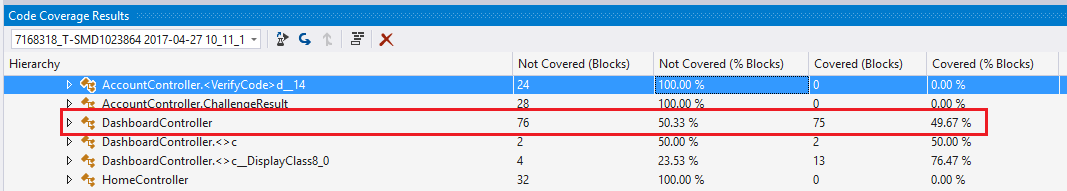
\includegraphics[scale=0.45]{./webAppCodeCoverage.png}
  \caption{Code Coverage for Dashboard Controller}
 \label{fig:webappCodeCoverage}
\end{figure}

\subsection{Web API}
When tested, the Web API had the following successes, issues, and problems:\\\\
Successes
\begin{itemize}
\item The controllers that were written for this project are 100\% unit tested and 98\% unit tested. The given code and controllers from Microsoft when creating the web API project was not unit tested
\end{itemize}
Issues
\begin{itemize}
\item Not all the controllers are 100\% unit tested.
\end{itemize}
Problems
\begin{itemize}
\item Figuring out how to throw certain exceptions while using Moq.
\end{itemize}
The following figures depict the unit test coverage results:

\begin{figure}[h!]
\centering
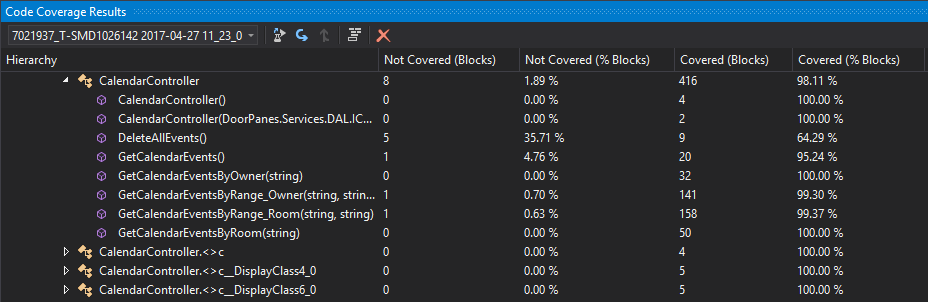
\includegraphics[width=0.75\textwidth]{./DetailCalendarCoverage.PNG}
\caption{Code Coverage for Calendar Controller}
\label{CalendarControllerCoverage}
\end{figure}

\begin{figure}[h!]
\centering
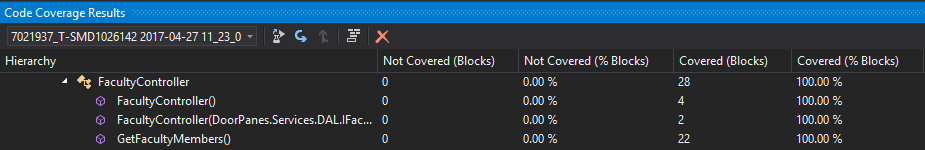
\includegraphics[width=0.75\textwidth]{./DetailFacultyCoverage.PNG}
\caption{Code Coverage for Faculty Controller}
\label{FacultyControllerCoverage}
\end{figure}

\begin{figure}[h!]
\centering
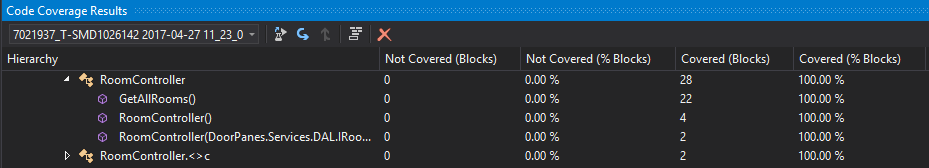
\includegraphics[width=0.75\textwidth]{./DetailRoomCoverage.PNG}
\caption{Code Coverage for Room Controller}
\label{RoomControllerCoverage}
\end{figure}

\subsection{Tablet Application}
When tested, the tablet application had the following successes, issues, and problems:\\\\
Successes
\begin{itemize}
\item Unit tested all possible inputs for log in page
\item Ran UI tests for all UI elements
\end{itemize}
Issues
\begin{itemize}
\item Unable to mock data that is being received using API calls.  So as of now it is assumed that the data coming in is correct and in the right format.
\end{itemize}
Problems
\begin{itemize}
\item Learning curve in making UI tests as it was unsure exactly how to test that.
\end{itemize}

  %% All tracks
% !TEX root = DesignDocument.tex


\chapter{Prototypes}

\begin{comment}This chapter is for recording each prototype developed.  It is a historical record of what you accomplished in 464/465.   This should be organized according to Sprints.  It should have the basic description of the sprint deliverable and what was accomplished.  Screen shots, photos, captures from video, etc should be used. 
\end{comment} 

\section{Sprint 1 Prototype}
\subsection{Deliverables}
\begin{itemize}
\item Software Contract
\item Sprint Report 1
\item Hardware Decision
\end{itemize}

\subsection{Backlog}
\subsection*{Azure}
\begin{itemize}
\item Set up Azure
\item Create Azure database
\item User Authentication
\item App Communication
\end{itemize}

\subsection*{Web Application}
\begin{itemize}
\item Create Web App project
\item Upload Web App project to Azure
\item Create website login screen
\item Communicate with Azure
\item Create schedule templates
\item \#14: Update Web App Homepage 
\item \#20: Create Dashboard View
\item \#21: Revamp Login and Register Web App Pages 
\item \#30 Web App - Open calendar framework JSON events
\item \#31 Web App - Connect calendar event creation to database
\item \#33 Web App - Load events from database when navigating to dashboard controller
\item \#34: Web App - Remove authorization code
\item \#35 Create Unit test projects for both the web applications and web API projects
\item \#37 Web App (TEAM) - Create wireframe for design
\item Code the user interface according to wireframes
\item \#58 Web App - Add code to insert calendar events into database
\item \#59 Web App - Grab JSON from calendar framework
\item \#60 Web App - Load events from database
\item Create distinguished views for each type of user
\item Role based detection
\item Registration process
\item Database table integration and referencing
\item Repetition to generate repeated calendar events
\item Handle temporary canceled events
\end{itemize}

\subsection*{Web API}
\begin{itemize}
\item Create Web API project
\item Update Web API project to Azure
\item Model Location
\item Repository Layer
\item Serialize data
\item Migration on database
\item Create API endpoints for moving schedule data back and forth
\item \#24 Web API - Create Professor Model
\item \#25 Web API - Create Office Personnel Model
\item \#26 Web API - Create Calendar Event Model
\item \#27 Web API - Model Location
\item \#28 Web API - Create GetCalendarEvent endpoint
\item \#29 Web API - Create GetCalendarEvents endpoint
\item \#32 Web API - Create SaveCalendarEvents endpoint
\item \#35 Create Unit test projects for both the web applications and web API projects
\item \#41 Web API - Repository Layer
\item \#43 Web API - Serialize data
\item \#61 Web API - Fix Models
\item \#62 Web API - Create GetCalendarEventsByOwner endpoint
\item \#64 Web API - Create GetCalendarEventsByRoom
\item \#67 Web API - Display options endpoints
\item \#68 Web API - Create GetCalendarEventsByRange
\item \#69 Web API - Model updates
\item Testing
\end{itemize}

\subsection*{Tablet Application}
\begin{itemize}
\item Design and create splash screen
\item Enable tablet to connect to Azure
\item Create communication class
\item Display a message on tablet screen
\item Display schedule on tablet	
\item Learn XamarinLearn Xamarin\footnote{See Appendix \ref{XamarinAppendix}\label{note4}}
\item Create Xamarin tablet application with a login page\textsuperscript{\ref{note4}}
\item \#17 Create Xamarin Tablet App
\item \#18 Tablet App - Android Kiosk Mode for Tablet App
\item \#19 Second Tablet App View
\item \#36 Tablet App - Create Calendar View
\item \#38 Tablet App (TEAM) - Create wireframe for tablet app
\item Code the user interface according to wireframes
\item \#39 Tablet App - Create communications class
\item \#40 Tablet App - Create a way to display JSON calendar events
\item \#42 Tablet App - Move Tablet Code
\item \#53 Android calendar framework JSON function
\item Create pop-up window with description
\item Modify week view class open source
\item Added synchronization button
\item Implement continuous synchronization
\item Create login page
\item Add a view to select calendar based on faculty or room
\item Token authentication
\item GUI modifications
\item Handle temporary canceled events
\item Testing
\end{itemize}

\subsection*{Miscellaneous}
\begin{itemize}
\item Logo
\item Research Tablet vs Odroid Options
\item Connect Visual Studio to Azure
\item Look into networking for tablets
\item Look into a pre-built calendar framework for displaying calendar events
\item Create middleman project
\item Make sure system is very secure
\item \#54 Understand how event ownership works
\end{itemize}

\subsection{Success/Fail}
Our success was understanding and combining the visions of the clients.


\section{Sprint 2 Prototype}
\subsection{Web Application}
\subsubsection{Deliverable}
By the end of sprint 2, we wanted to have an ASP.NET Web App project hosted in Azure and accessible via a URL. In addition, we also wanted to be able to navigate to a "dashboard" view on the web app site that would allow a user to see a weekly display of calendar events.
\subsubsection{Backlog}
\begin{itemize}
\item Upload Web App project to Azure
\item Create website login screen
\item Communicate with Azure
\item Create schedule templates
\item \#14: Update Web App Homepage - For this issue, the web app homepage was updated from the stock web app template to reflect the DoorPanes project. The text and the site colors were updated under this issue.
\item \#20: Create Dashboard View - For this issue, a dashboard controller and a dashboard view were added to the web app project. Once this was done, a user could navigate to the dashboard controller and see a listing of calendar events.
\item \#21: Revamp Login and Register Web App Pages - For this issue, the login page and the register page were updated to reflect the homepage design.
\item \#30 Web App - Open calendar framework JSON events
\item \#31 Web App - Connect calendar event creation to database
\item \#33 Web App - Load events from database when navigating to dashboard controller
\item \#34: Web App - Remove authorization code
\item \#35 Create Unit test projects for both the web applications and web API projects
\item \#37 Web App (TEAM) - Create wireframe for design
\item Code the user interface according to wireframes
\item \#58 Web App - Add code to insert calendar events into database
\item \#59 Web App - Grab JSON from calendar framework
\item \#60 Web App - Load events from database
\item Create distinguished views for each type of user
\item Role based detection
\item Registration process
\item Database table integration and referencing
\item Repetition to generate repeated calendar events
\item Handle temporary canceled events
\end{itemize}


%The items in that were in the backlog for sprint 2 for the Web App were as follows:

%\begin{itemize}
%\item Issue \#14: Update Web App Homepage - For this issue, the web app homepage was updated from the stock web app template to reflect the DoorPanes project. The text and the site colors were updated under this issue.
%\item Issue \#20: Create Dashboard View - For this issue, a dashboard controller and a dashboard view were added to the web app project. Once this was done, a user could navigate to the dashboard controller and see a listing of calendar events.
%\item Issue \#21: Revamp Login and Register Web App Pages - For this issue, the login page and the register page were updated to reflect the homepage design. 
%\end{itemize}

\subsubsection{Success/Fail}
All of the issues pertaining to the web app for sprint 2 were accomplished during Sprint 2.

\subsection{Web API}
\subsubsection{Deliverable}
The Web API project was created.
\subsubsection{Backlog}
\begin{itemize}
\item Create Web API project
\item Update Web API project to Azure
\item Model Location
\item Repository Layer
\item Serialize data
\item Migration on database
\item Create API endpoints for moving schedule data back and forth
\item \#16: Create MVC models
\item \#22: Create API endpoints
\item \#24 Web API - Create Professor Model
\item \#25 Web API - Create Office Personnel Model
\item \#26 Web API - Create Calendar Event Model
\item \#27 Web API - Model Location
\item \#28 Web API - Create GetCalendarEvent endpoint
\item \#29 Web API - Create GetCalendarEvents endpoint
\item \#32 Web API - Create SaveCalendarEvents endpoint
\item \#35 Create Unit test projects for both the web applications and web API projects
\item \#41 Web API - Repository Layer
\item \#43 Web API - Serialize data
\item \#61 Web API - Fix Models
\item \#62 Web API - Create GetCalendarEventsByOwner endpoint
\item \#64 Web API - Create GetCalendarEventsByRoom
\item \#67 Web API - Display options endpoints
\item \#68 Web API - Create GetCalendarEventsByRange
\item \#69 Web API - Model updates
\item Testing
\end{itemize}

\subsubsection{Success/Fail}
Our success was finally understanding the necessary steps to implement the API models and controllers. Another success was figuring out how the API connected to the database. We failed at getting a good start on the API in this sprint. We also realized we needed to break the backlog down into more specific tasks.

\subsection{Tablet Application}
\subsubsection{Deliverable}
During Sprint 2, our tablet application was being developed using Xamarin. We fell into many issues getting the Xamarin environment to be set up correctly. We were unable to develop a working application during this sprint.  However, our idea for the look of this application is shown in Figure \ref{fig:firstview} and Figure \ref{fig:navdrawer}. 

\begin{figure}
\centering
  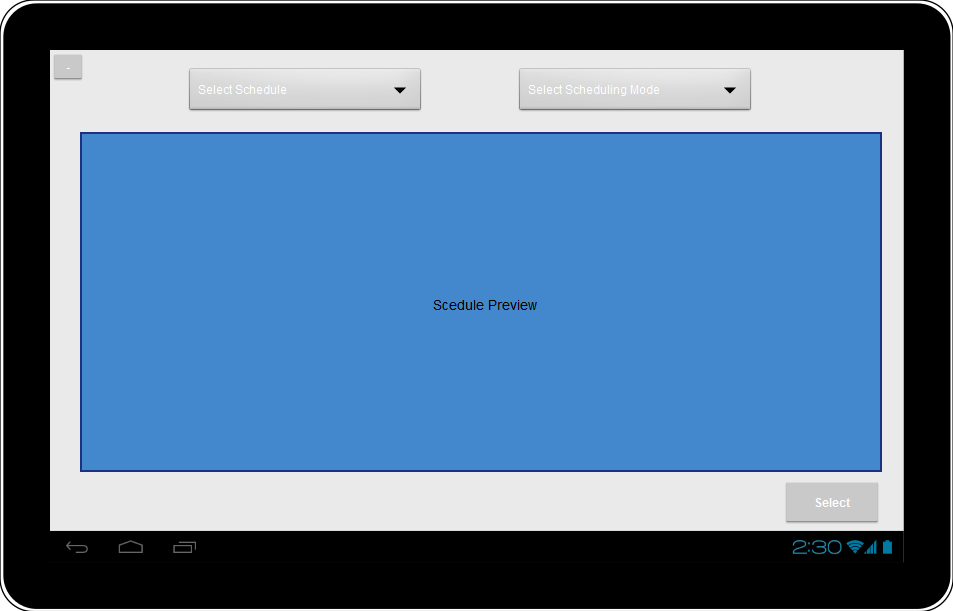
\includegraphics[scale=0.45]{firstview.png}
  \caption{Preview Page}
  \label{fig:firstview}
\end{figure}

\begin{figure}
\centering
  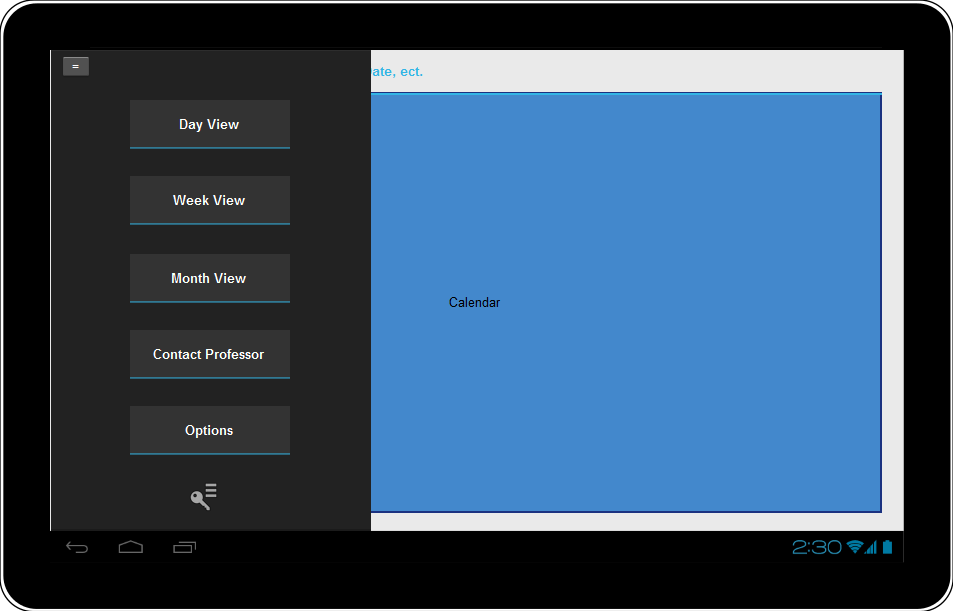
\includegraphics[scale=0.45]{navigationdrawer.png}
  \caption{Dashboard view with navigation drawer expanded}
  \label{fig:navdrawer}
\end{figure}
\subsubsection{Backlog}
\begin{itemize}
\item Design and create splash screen
\item Enable tablet to connect to Azure
\item Display a message on tablet screen
\item Display schedule on tablet	
\item Learn XamarinLearn Xamarin\footnote{See Appendix \ref{XamarinAppendix}\label{note2}}
\item Create Xamarin tablet application with a login page\textsuperscript{\ref{note2}}
\item \#17 Create Xamarin Tablet App
\item \#18 Tablet App - Android Kiosk Mode for Tablet App
item \#19 Second Tablet App View
\item \#36 Tablet App - Create Calendar View
\item \#38 Tablet App (TEAM) - Create wireframe for tablet app
\item Code the user interface according to wireframes
\item \#39 Tablet App - Create communications class
\item \#40 Tablet App - Create a way to display JSON calendar events
\item \#42 Tablet App - Move Tablet Code
\item \#53 Android calendar framework JSON function
\item Create pop-up window with description
\item Modify week view class open source
\item Added synchronization button
\item Implement continuous synchronization
\item Create login page
\item Add a view to select calendar based on faculty or room
\item Token authentication
\item GUI modifications
\item Handle temporary canceled events
\item Testing
\end{itemize}

\subsubsection{Success/Fail}
At the end of this sprint it was decide we were no longer going to use Xamarin to develop our tablet application.  All future development will be done using Android Studio.  The little work that was accomplished in Xamarin will be transferred to native Android.

\subsection*{Miscellaneous Backlog}
\begin{itemize}
\item Logo
\item Connect Visual Studio to Azure
\item Look into networking for tablets
\item Create middleman project
\item Make sure system is very secure
\item \#54 Understand how event ownership works
\end{itemize}

\section{Sprint 3 Prototype}
\subsection{Web Application}
\subsubsection{Deliverable}
By the end of sprint 3, we wanted to have the ability to add and remove calendar events from the dashboard controller and have the changes made to the dashboard calender event view persist when a user closed the browser window/tab.
\subsubsection{Backlog}
\begin{itemize}
\item \#30 Web App  - Open calendar framework JSON events. For this issue, we needed to understand how the open source calendar framework we were using stored JSON calendar events.
\item \#31 Web App - Connect calendar event creation to database. For this issue, the calendar event creation mechanism in the open source calendar framework needed to be connected to an endpoint that would create a calendar event model and store it in the database.
\item \#33 Web App - Load events from database when navigating to dashboard controller. For this issue, the load event hook in the open source calendar framework needed to be connected to the get calendar events web app endpoint so events could be loaded from the database when the user navigated to the dashboard page.
\item \#34: Web App - Remove authorization code. For this issue, the authorization code was removed from the web app so data-flow development could happen without needing to worry about being authorized yet. The authorization code will be added in at a later date.
\item \#35 Create Unit test projects for both the web applications and web API projects
\item \#37 Web App (TEAM) - Create wireframe for design
\item Code the user interface according to wireframes
\item \#58 Web App - Add code to insert calendar events into database
\item \#59 Web App - Grab JSON from calendar framework
\item \#60 Web App - Load events from database
\item Create distinguished views for each type of user
\item Role based detection
\item Registration process
\item Database table integration and referencing
\item Repetition to generate repeated calendar events
\item Handle temporary canceled events
\end{itemize}

%The issues that were in the backlog for sprint 3 for the Web App were as follows:

%\begin{itemize}
%\item Issue \#30: Web App - Open calendar framework JSON events. For this issue, we needed to understand how the open source calendar framework we were using stored JSON calendar events.
%\item Issue \#31: Web App - Connect calendar event creation to database. For this issue, the calendar event creation mechanism in the open source calendar framework needed to be connected to an endpoint that would create a calendar event model and store it in the database.
%\item Issue \#33: Web App - Load events from database when navigating to dashboard controller. For this issue, the load event hook in the open source calendar framework needed to be connected to the get calendar events web app endpoint so events could be loaded from the database when the user navigated to the dashboard page.
%\item Issue \#34: Web App - Remove authorization code. For this issue, the authorization code was removed from the web app so data-flow development could happen without needing to worry about being authorized yet. The authorization code will be added in at a later date.
%\end{itemize}

\subsubsection{Success/Fail}
Due to struggles with the API endpoint creation and major issues with the tablet app, the only issue that was resolved was Issue \#30 (understanding the JSON event storage in the open source calendar framework). The remaining issues will have to be moved to a later sprint.

\subsection{Web API}
\subsubsection{Deliverable}
The following was created and implemented in this sprint:
Endpoints
\begin{itemize}
\item Get Calendar Events By Owner
\item Get Calendar Events
\item Save Calendar Events
\end{itemize}
Models
\begin{itemize}
\item Office Personnel Model
\item Instructor Model
\item Person Model
\item Event Model
\end{itemize}
\subsubsection{Backlog}
\begin{itemize}
\item Create Web API project
\item Update Web API project to Azure
\item Model Location
\item Repository Layer
\item Migration on database
\item Create API endpoints for moving schedule data back and forth
\item \#24 Web API - Create Professor Model
\item \#25 Web API - Create Office Personnel Model
\item \#26 Web API - Create Calendar Event Model
\item \#27 Web API - Model Location
\item \#28 Web API - Create GetCalendarEvent endpoint
\item \#29 Web API - Create GetCalendarEvents endpoint
\item \#32 Web API - Create SaveCalendarEvents endpoint
\item \#35 Create Unit test projects for both the web applications and web API projects
\item \#41 Web API - Repository Layer
\item \#43 Web API - Serialize data
\item \#61 Web API - Fix Models
\item \#62 Web API - Create GetCalendarEventsByOwner endpoint
\item \#64 Web API - Create GetCalendarEventsByRoom
\item \#67 Web API - Display options endpoints
\item \#68 Web API - Create GetCalendarEventsByRange
\item \#69 Web API - Model updates
\item Testing
\end{itemize}

\subsubsection{Success/Fail}
Our success in this sprint for the web API component was that everything in the backlog was completed or nearly  completed.

\subsection{Tablet Application}
\subsubsection{Deliverable}
Once switched over to native Android, development went a lot smoother.  A wireframe model was developed including a good portion of the features needed for our finished product.  The screenshots of our prototype are shown starting with Figure ~\ref{fig:loginscreen}.  One upgrade in Android Studio as opposed to Xamarin, is the implementation of activities.  An activity is a single, focused thing the user can do.  The use of activites allows for the user to switch between screen views, rotate the tablet, switch to another application, and the state of the app is saved and restarted when any said action occurs.  It was more difficult to create these activites using Xamarin.  



\begin{figure}
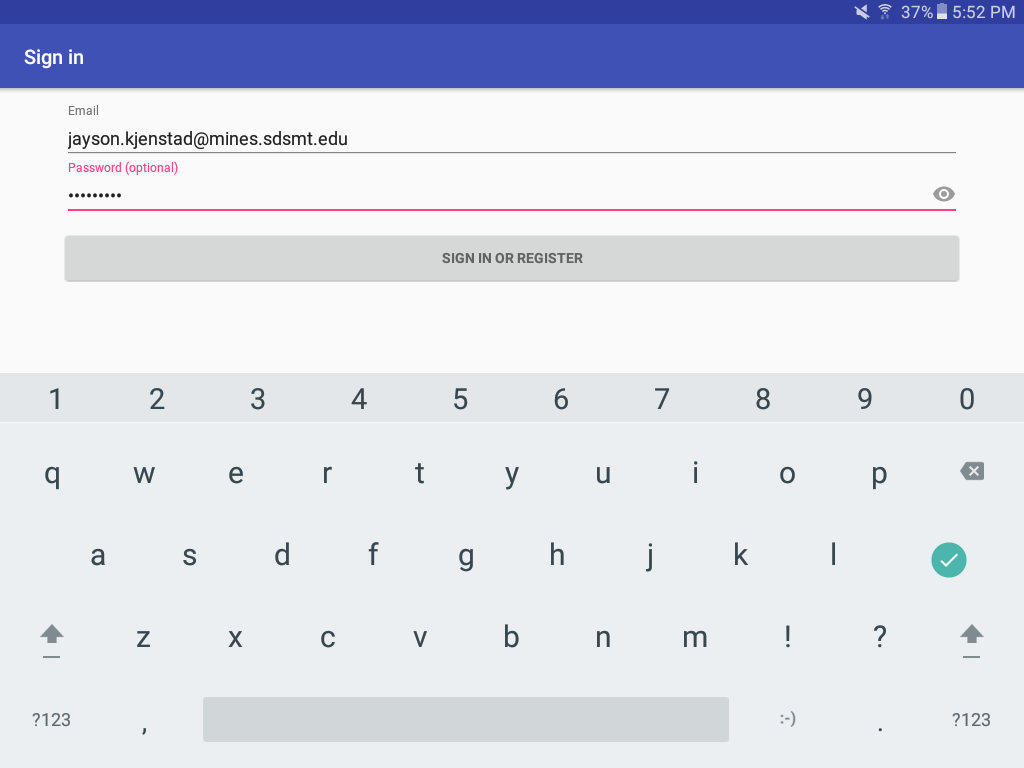
\includegraphics[scale=0.45]{loginscreen.png}
\caption{Login screen}
\label{fig:loginscreen}
\end{figure}

\begin{figure}
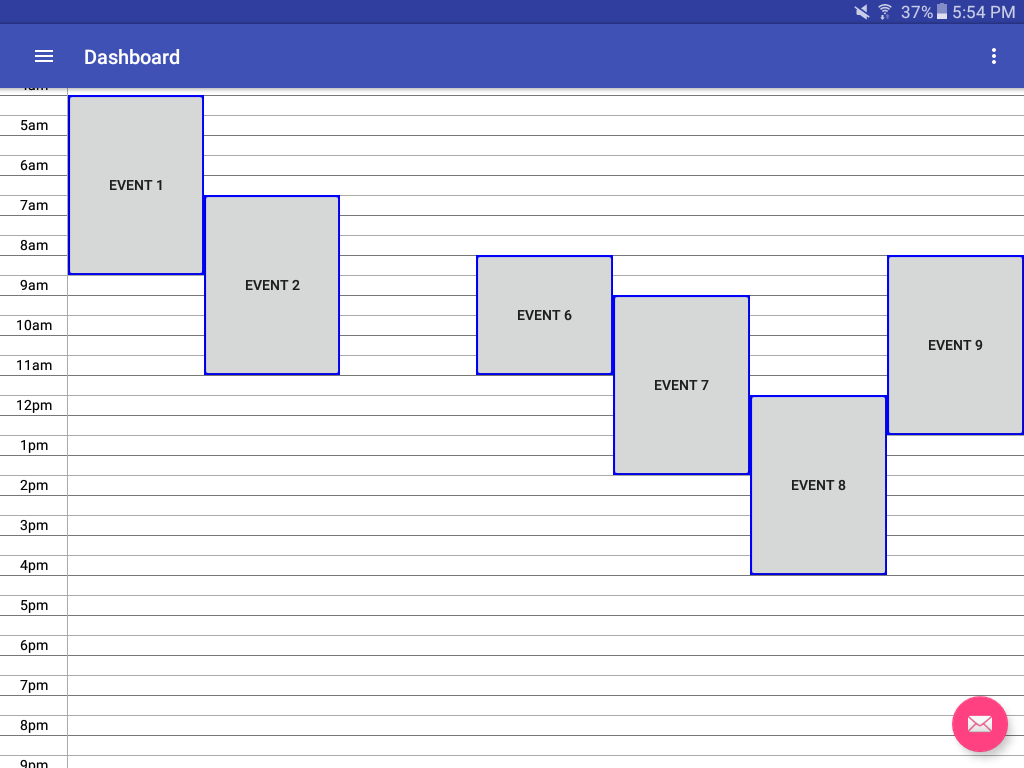
\includegraphics[scale=0.45]{calendarview.png}
\caption{Calendar view with events}
\label{fig:calendar}
\end{figure}

\begin{figure}
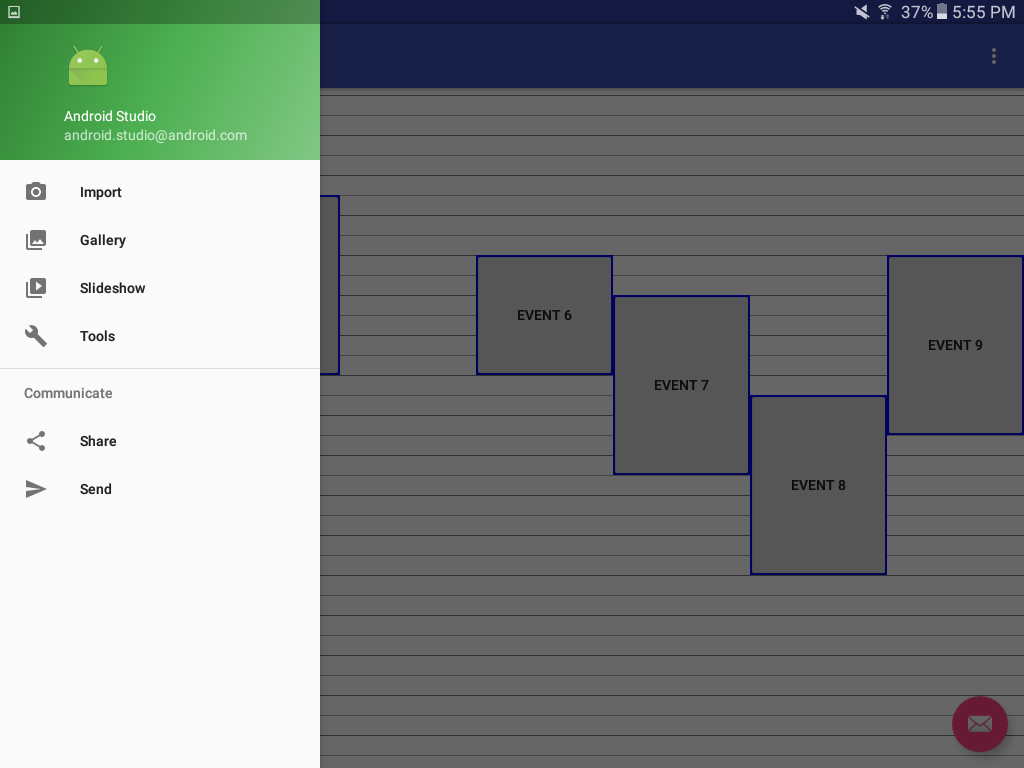
\includegraphics[scale=0.45]
{navigation.png}
\caption{Dashboard view with navigation drawer expanded}
\label{fig:nav}
\end{figure}

\subsubsection{Backlog}
\begin{itemize}
\item Design and create splash screen
\item Enable tablet to connect to Azure
\item Display a message on tablet screen
\item Display schedule on tablet	
\item Learn XamarinLearn Xamarin\footnote{See Appendix \ref{XamarinAppendix}\label{note3}}
\item Create Xamarin tablet application with a login page\textsuperscript{\ref{note3}}
\item \#18 Tablet App - Android Kiosk Mode for Tablet App
\item \#36 Tablet App - Create Calendar View
\item \#38 Tablet App (TEAM) - Create wireframe for tablet app
\item Code the user interface according to wireframes
\item \#39 Tablet App - Create communications class
\item \#40 Tablet App - Create a way to display JSON calendar events
\item \#42 Tablet App - Move Tablet Code
\item \#53 Android calendar framework JSON function
\item Create pop-up window with description
\item Modify week view class open source
\item Added synchronization button
\item Implement continuous synchronization
\item Create login page
\item Add a view to select calendar based on faculty or room
\item Token authentication
\item GUI modifications
\item Handle temporary canceled events
\item Testing
\end{itemize}

\subsubsection{Success/Fail}
A wireframe for a good portion of the application was created.  A calendar view was created where the JSON calendar events can be displayed as a button on the view.  However, there was no actual integration of the JSON events yet.  That and the communications class will be pushed to our sprint after winter break.

\subsection*{Miscellaneous Backlog}
\begin{itemize}
\item Logo
\item Research Tablet vs Odroid Options
\item Connect Visual Studio to Azure
\item Look into networking for tablets
\item Look into a pre-built calendar framework for displaying calendar events
\item Create middleman project
\item Make sure system is very secure
\item \#54 Understand how event ownership works
\end{itemize}

\section{Sprint 4 Prototype}

\subsection{Web Application}
\subsubsection{Deliverable}
The following were delivered for this sprint:
\begin{itemize}
\item Load events from database
\item Connect web application database to Azure
\item Created middle man project for web application and web API to share
\item Display calendar events on the calendar framework on the web application
\end{itemize}

\subsubsection{Backlog}
The backlog for the web app is the following:
\begin{itemize}
\item \#33 Web App - Load events from database when navigating to dashboard controller
\item \#35 Create Unit test projects for both the web applications and web API projects
\item \#37 Web App (TEAM) - Create wireframe for design
\item Code the user interface according to wireframes
\item \#58 Web App - Add code to insert calendar events into database
\item \#59 Web App - Grab JSON from calendar framework
\item \#60 Web App - Load events from database
\item Create distinguished views for each type of user
\item Role based detection
\item Registration process
\item Database table integration and referencing
\item Repetition to generate repeated calendar events
\item Handle temporary canceled events
\end{itemize}

\subsubsection{Success/Fail}
Some items we fell short on during this sprint were understanding database seeding and migrations problems, GUID usage, and database permissions and authorization.

\subsection{Web API}
\subsubsection{Deliverable}
The following were delivered for this sprint:
\begin{itemize}
\item Return actual JSON from web API endpoints
\item Updated getByOwner endpoint
\item Updated web API models
\item Understand GUID principles
\end{itemize}

\subsubsection{Backlog}
The backlog for the web API is the following:
\begin{itemize}
\item Repository Layer
\item Migration on database
\item \#35 Create Unit test projects for both the web applications and web API projects
\item \#41 Web API - Repository Layer
\item \#43 Web API - Serialize data
\item \#61 Web API - Fix Models
\item \#62 Web API - Create GetCalendarEventsByOwner endpoint
\item \#64 Web API - Create GetCalendarEventsByRoom
\item \#67 Web API - Display options endpoints
\item \#68 Web API - Create GetCalendarEventsByRange
\item \#69 Web API - Model updates
\item Testing
\end{itemize}

\subsubsection{Success/Fail}
Some setbacks we encountered during this sprint were understanding database seeding and migrations problems (didn't understand how they worked), GUID usage, and database permissions and authorization.

\subsection{Tablet Application}
\subsubsection{Deliverable}
The following were delivered for this sprint:
\begin{itemize}
\item Making a get request to an Azure server from the tablet application and getting JSON returned
\item Displaying JSON calendar events on the tablet application screen
\item Understand tablet class layout
\end{itemize}

\subsubsection{Backlog}
\begin{itemize}
\item Enable tablet to connect to Azure
\item Display a message on tablet screen
\item Display schedule on tablet	
\item \#18 Tablet App - Android Kiosk Mode for Tablet App
\item \#36 Tablet App - Create Calendar View
\item \#38 Tablet App (TEAM) - Create wireframe for tablet app
\item Code the user interface according to wireframes
\item \#39 Tablet App - Create communications class
\item \#40 Tablet App - Create a way to display JSON calendar events
\item \#53 Android calendar framework JSON function
\item Create pop-up window with description
\item Modify week view class open source
\item Added synchronization button
\item Token authentication
\item GUI modifications
\item Handle temporary canceled events
\item Testing
\end{itemize}

\subsubsection{Success/Fail}
One setback for the tablet application was the amount of time it took understanding and working out retrofit requests.

\subsection*{Miscellaneous Backlog}
\begin{itemize}
\item Logo
\item Look into networking for tablets
\item Make sure system is very secure
\item \#54 Understand how event ownership works
\end{itemize} 

\section{Sprint 5 Prototype}
\subsection{Web Application}

\subsubsection{Deliverable}
The following were delivered for this sprint:
\begin{itemize}
\item Calendar event creation
\item Partially unit tested
\item Save events
\end{itemize}
\subsubsection{Backlog}
\begin{itemize}
\item \#33 Web App - Load events from database when navigating to dashboard controller
\item \#35 Create Unit test projects for both the web applications and web API projects
\item \#37 Web App (TEAM) - Create wireframe for design
\item Code the user interface according to wireframes
\item \#58 Web App - Add code to insert calendar events into database
\item \#59 Web App - Grab JSON from calendar framework
\item \#60 Web App - Load events from database
\item Create distinguished views for each type of user
\item Role based detection
\item Registration process
\item Database table integration and referencing
\item Repetition to generate repeated calendar events
\item Handle temporary canceled events
\end{itemize}

\subsection{Web API}
\subsubsection{Deliverable}
The following were delivered for this sprint:
\begin{itemize}
\item Unit Tested the current endpoints
\item Create Get calendar events by room
\end{itemize}

\subsubsection{Backlog}
\begin{itemize}
\item Repository Layer
\item Migration on database
\item \#35 Create Unit test projects for both the web applications and web API projects
\item \#64 Web API - Create GetCalendarEventsByRoom
\item \#67 Web API - Display options endpoints
\item \#68 Web API - Create GetCalendarEventsByRange
\item \#69 Web API - Model updates
\item Testing
\end{itemize}

\subsubsection{Success/Fail}
The GetCalendarEventsByRange endpoint was delayed and pushed to the final sprint.

\subsection{Tablet Application}
\subsubsection{Deliverable}
The following were delivered for this sprint:
\begin{itemize}
\item Calendar event synchronization
\item GUI testing
\item Unit test for login screen
\item GUI modifications
\item Calendar description window
\end{itemize}
\subsubsection{Backlog}
\begin{itemize}
\item \#18 Tablet App - Android Kiosk Mode for Tablet App
\item Create pop-up window with description
\item Modify week view class open source
\item Implement continuous synchronization
\item Add a view to select calendar based on faculty or room
\item Token authentication
\item Handle temporary canceled events
\item Testing
\end{itemize}

\subsubsection{Success/Fail}
A setback for the tablet application this sprint was testing JSON responses

\subsection*{Miscellaneous Backlog}
\begin{itemize}
\item Logo
\item Look into networking for tablets
\item Make sure system is very secure
\item \#54 Understand how event ownership works
\end{itemize}

\section{Sprint 6 Prototype}
\subsection{Web Application}
\subsubsection{Deliverable}
The following were delivered for this sprint:
\begin{itemize}
\item Database table integration
\item Database table referencing
\item Person detection based on roles
\item Registration process
\item Different login views based on users
\item Repetition calendar event auto generated implemented but not used
\end{itemize}
\subsubsection{Backlog}
\begin{itemize}
\item Create distinguished views for each type of user
\item Role based detection
\item Registration process
\item Database table integration and referencing
\item Repetition to generate repeated calendar events
\item Handle temporary canceled events
\end{itemize}

\subsubsection{Success/Fail}
During this sprint JavaScript was used often for the continuing development of the web application. Therefore, learning more JavaScript was needed, slowing down progress.

\subsection{Web API}
\subsubsection{Deliverable}
The following were delivered for this sprint:
\begin{itemize}
\item Displays options for endpoint parameters
\item Created Get calendar events by range for room
\item Created Get calendar events by range for owner
\item Room table created
\item Updated models
\item Login and register enabled
\end{itemize}

\subsubsection{Backlog}
\begin{itemize}
\item Migration on database
\item \#67 Web API - Display options endpoints
\item \#68 Web API - Create GetCalendarEventsByRange
\item \#69 Web API - Model updates
\item Testing
\end{itemize}

\subsection{Tablet Application}
\subsubsection{Deliverable}
The following were delivered for this sprint:
\begin{itemize}
\item Added a view to select calendar based on faculty or room
\item Token authentication
\item GUI modifications
\end{itemize}
\subsubsection{Backlog}
\begin{itemize}
\item \#18 Tablet App - Android Kiosk Mode for Tablet App
\item Token authentication
\item Handle temporary canceled events
\end{itemize}

\subsubsection{Success/Fail}
The tablet application had a few hardware issues. 

\subsection*{Miscellaneous Backlog}
\begin{itemize}
\item Logo
\item Look into networking for tablets
\item Make sure system is very secure
\end{itemize}

\section{Final Prototype}

\subsection{Web APP}
The final prototype for the web application includes the ability to sign is as multiple users (instructors, staff, and students all have their own unique views). The final prototype also introduced the ability for staff members to add and view events for multiple rooms. Canceling events was also added in the final prototype. Other additional changes for this final prototype include setup and registration changes to indicate what role the person will be in when they sign up, JavaScript code refactoring and debugging, and calendar model changes to increase data flow flexibility. No major user interface changes were made other than slight HTML element tweaks to show the different views for the different roles. The final UI views for what the interface looks like can be viewed in the user document section of this document. 

\subsection{Web API}
The final prototype for the web API has several endpoints that are working correctly. The endpoints retrieve, save and delete events. The endpoints that get calendar events from the database have specifications except when retrieving all the events stored. A user can get calendar events based on the owner, room, and/or the semester. The API also has endpoints to return all the rooms and owners in the database. The controllers we wrote for the web API are 98\% unit tested

\subsection{Tablet App}
The final prototype for the tablet application has three main parts: login page, calendar select page, and the dashboard view.  The application starts at the login page where the user can enter in credentials made in the web application.  

\begin{figure}
  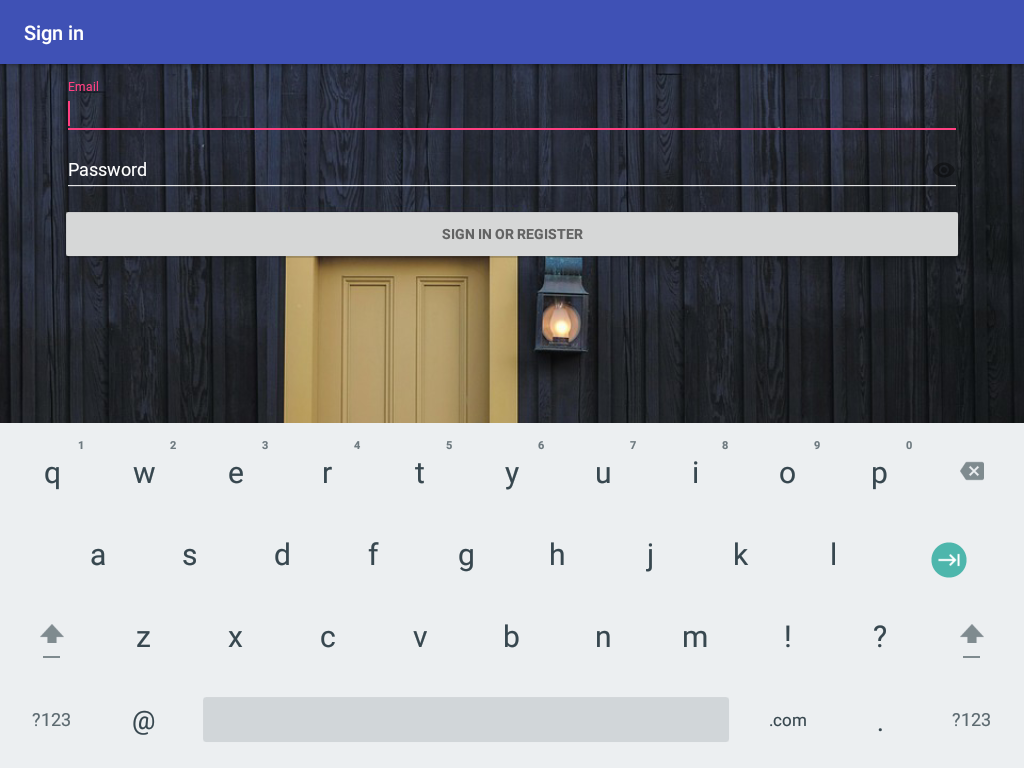
\includegraphics[scale=0.45]{login_final.png}
  \caption{Log in page for tablet application}
  \label{loginfinal}
\end{figure}

The page can be seen in Figure \ref{loginfinal}. On this page, the inputted credentials will be used in an API POST call.  If the password and the username match, a token is sent back in the response body.  This token needs to be used with all other API calls.  After a user logs in, the tablet shows the calendar selection view.  A list of all of the room and faculty schedules from the database are displayed in a dropdown menu.  Radio buttons switch between faculty and room lists.

\begin{figure}
  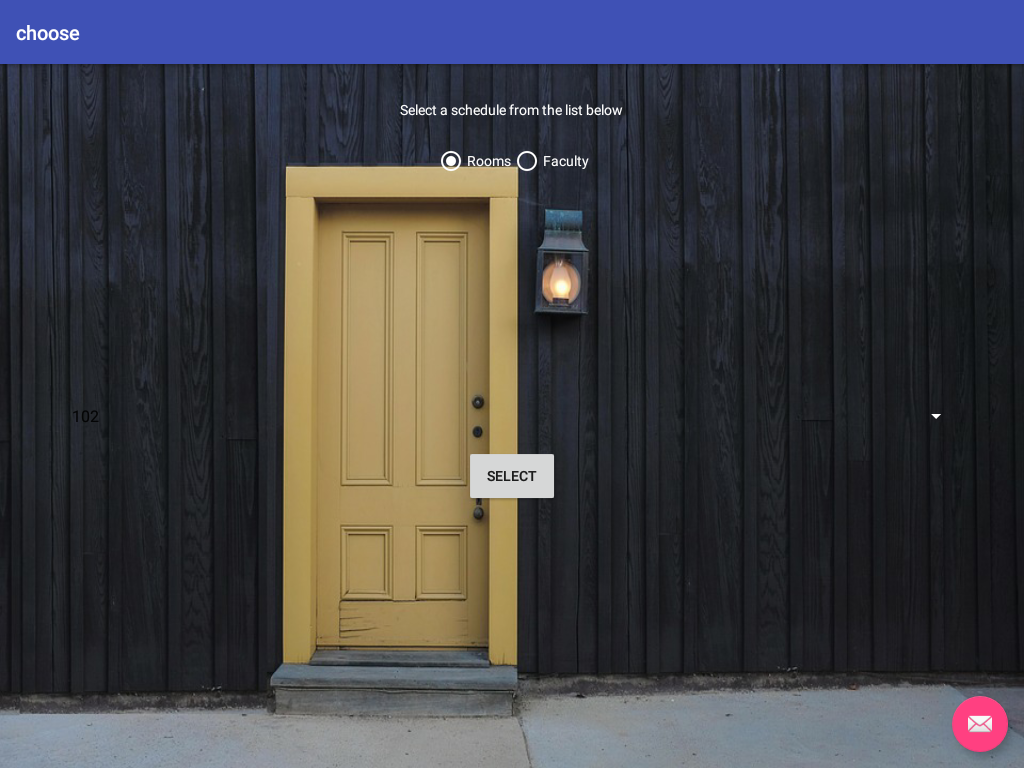
\includegraphics[scale=0.45]{selection_final.png}
  \caption{Calendar selection page for tablet application}
  \label{selectionfinal}
\end{figure}

This page is shown in Figure \ref{selectionfinal}.  After the schedule is selected, the given room or faculty schedule is saved and used for another API call to get all the calendar events.  On the next page, the user must first click the "Sync" button in the navigation drawer.  Once the button is pressed, every 10 seconds a request is sent to get the schedule again to continuously update.  

\begin{figure}
  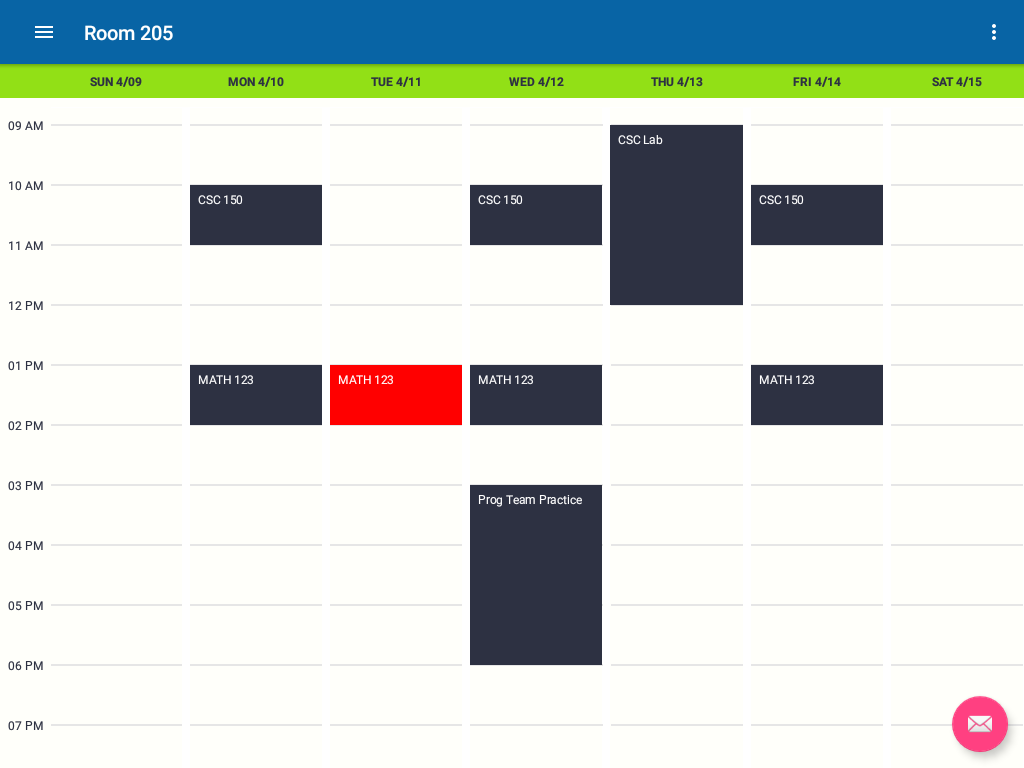
\includegraphics[scale=0.45]{dashboard_final.png}
  \caption{Final calendar view for tablet application}
  \label{dashboardfinal}
\end{figure}

This view can be seen in Figure \ref{dashboardfinal}. As mentioned the tablet will continuously update so it can be mounted and displayed on the proper door!





  %% All tracks
% !TEX encoding = UTF-8 Unicode
% !TEX root = DesignDocument.tex

\chapter{Release -- Setup -- Deployment}
This section should contain any specific subsection regarding specifics in releasing, 
setup, and/or deployment of the system. 


\section{Deployment Information and Dependencies}
Are there dependencies that are not embedded into the system install? 



\section{Setup Information}
How is a setup/install built? 



\section{System  Versioning Information}
How is the system versioned? 
  %% Normally not research track
% !TEX root = DesignDocument.tex

\chapter{User Documentation}

This section contains the end user documentation for the DoorPanes product. It covers the basic setup for using the product and where to go to find the product.

\section{User Guide}

The user guides for the Web Application and Tablet app are included in this section.

\begin{figure}
\centering
  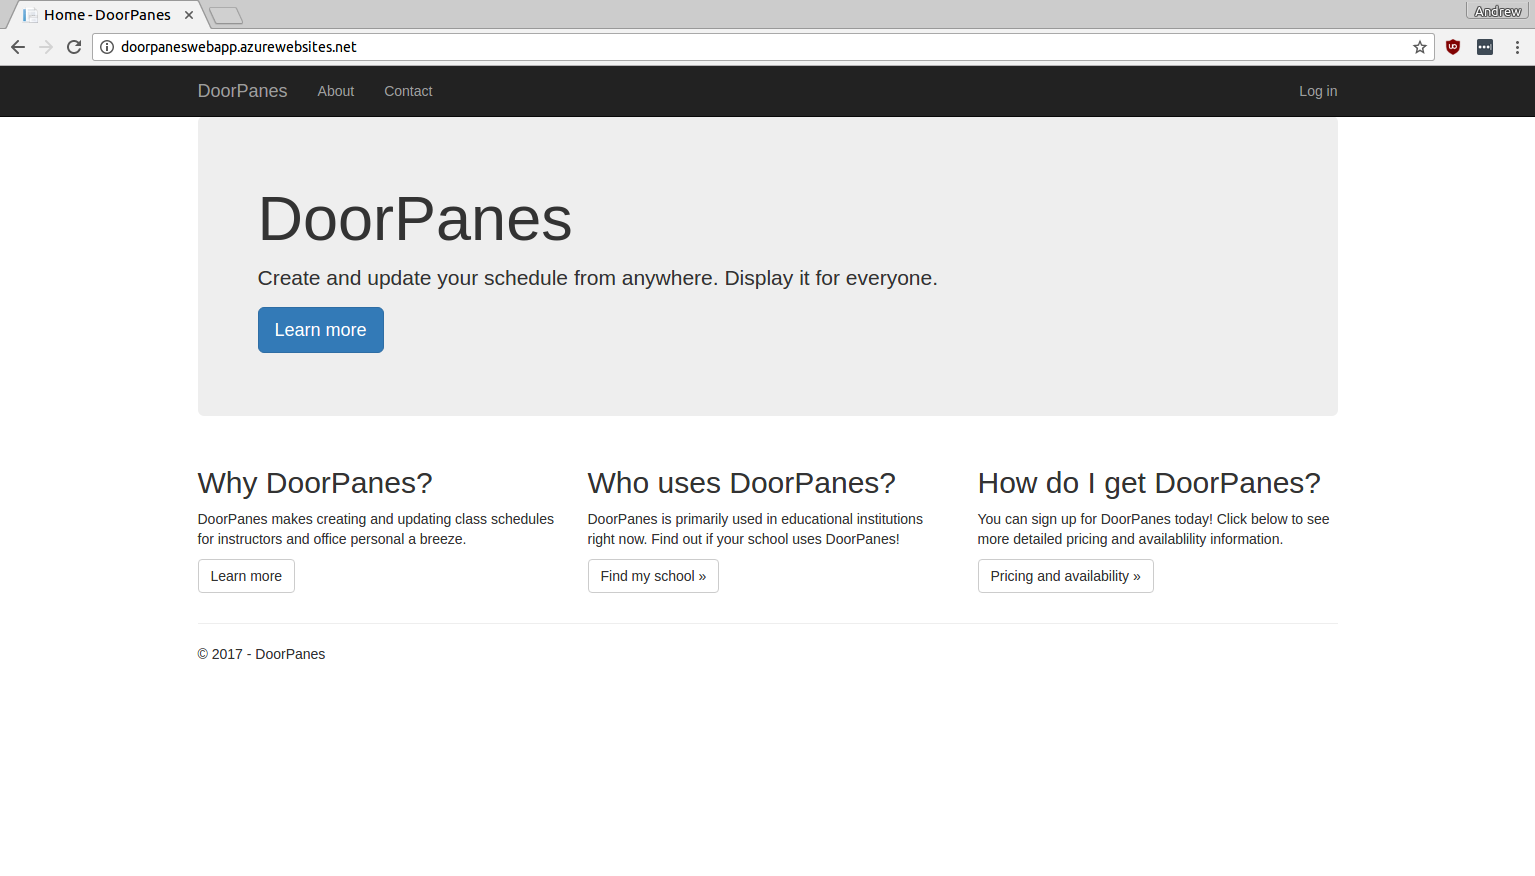
\includegraphics[scale=0.3]{DesignImages/UserGuideImagesWebApp/main_page.png}
  \caption{Main Web Page for Web App}
  \label{fig:main_page}
\end{figure}

\begin{figure}
\centering
  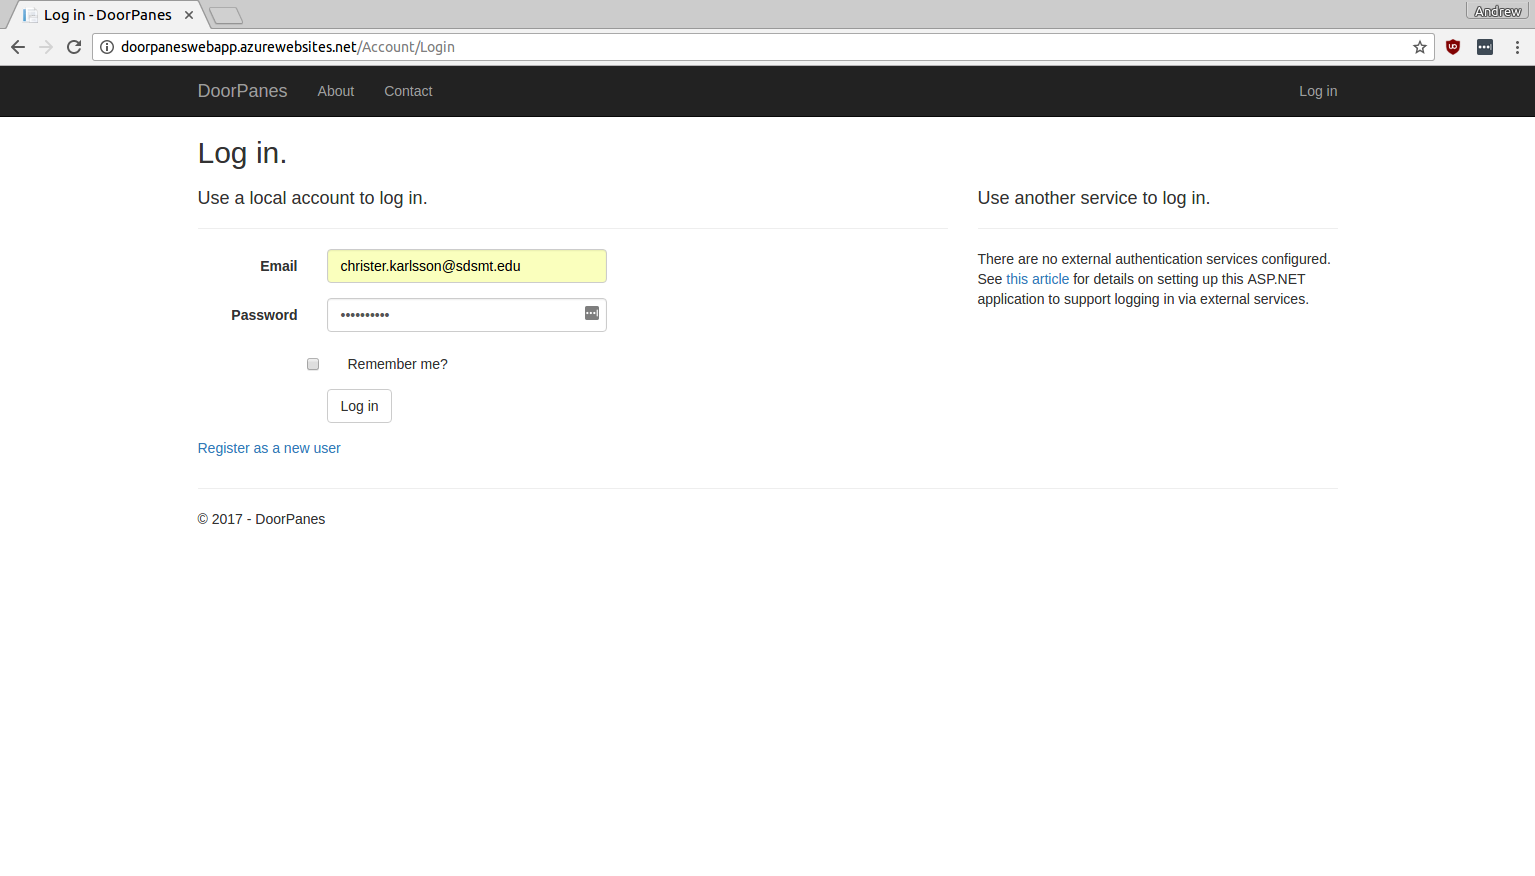
\includegraphics[scale=0.3]{DesignImages/UserGuideImagesWebApp/login_page.png}
  \caption{Main Login Page for Web App}
  \label{fig:login_page}
\end{figure}

\begin{figure}
\centering
  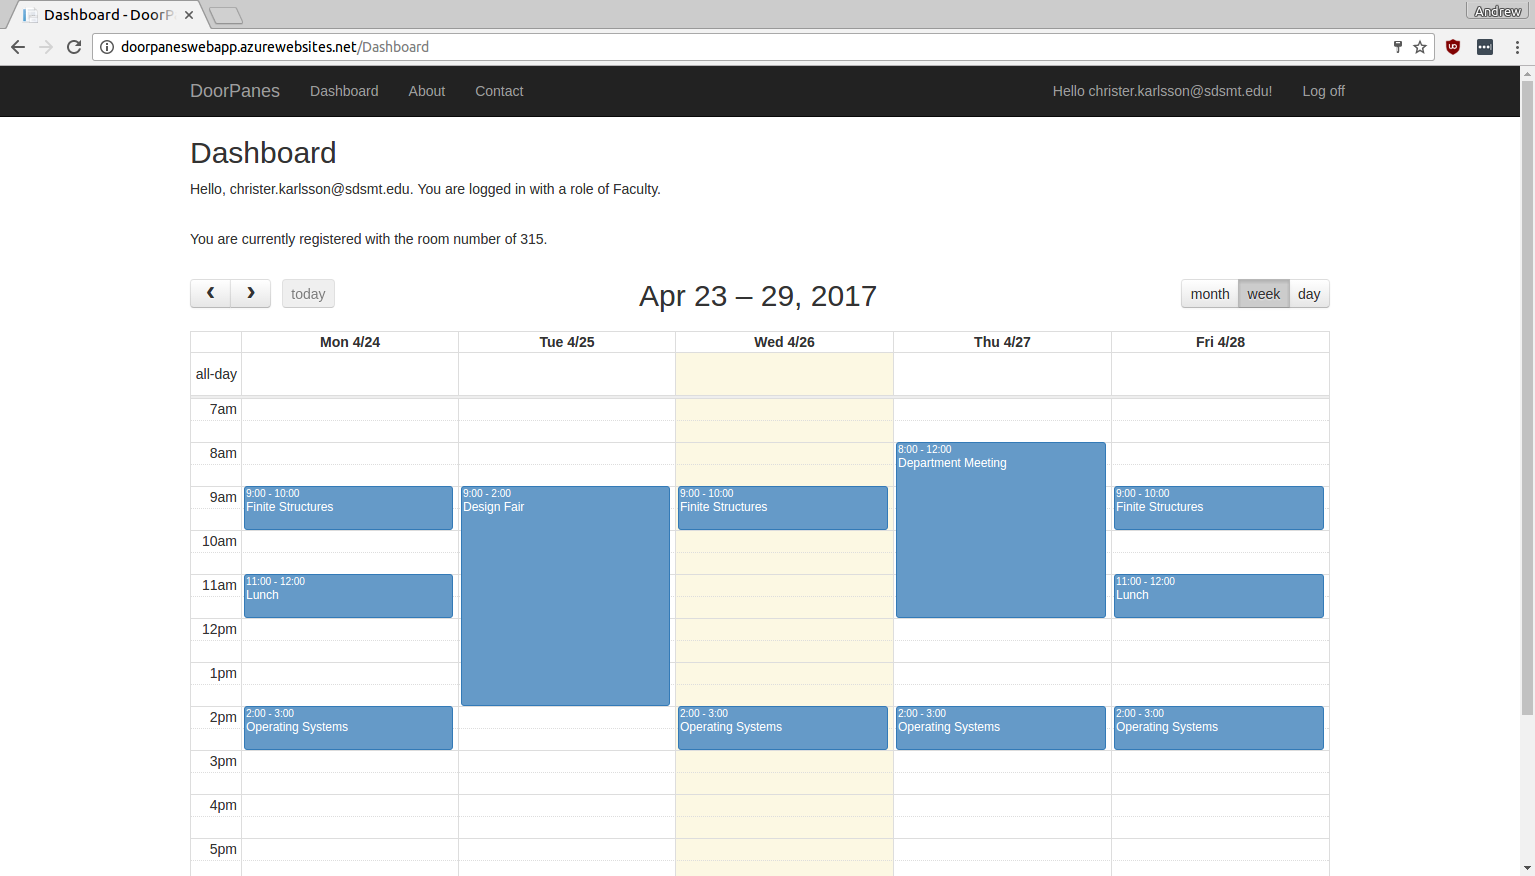
\includegraphics[scale=0.3]{DesignImages/UserGuideImagesWebApp/calendar_view.png}
  \caption{Web App Calendar View}
  \label{fig:calendar_view}
\end{figure}

\begin{figure}
\centering
  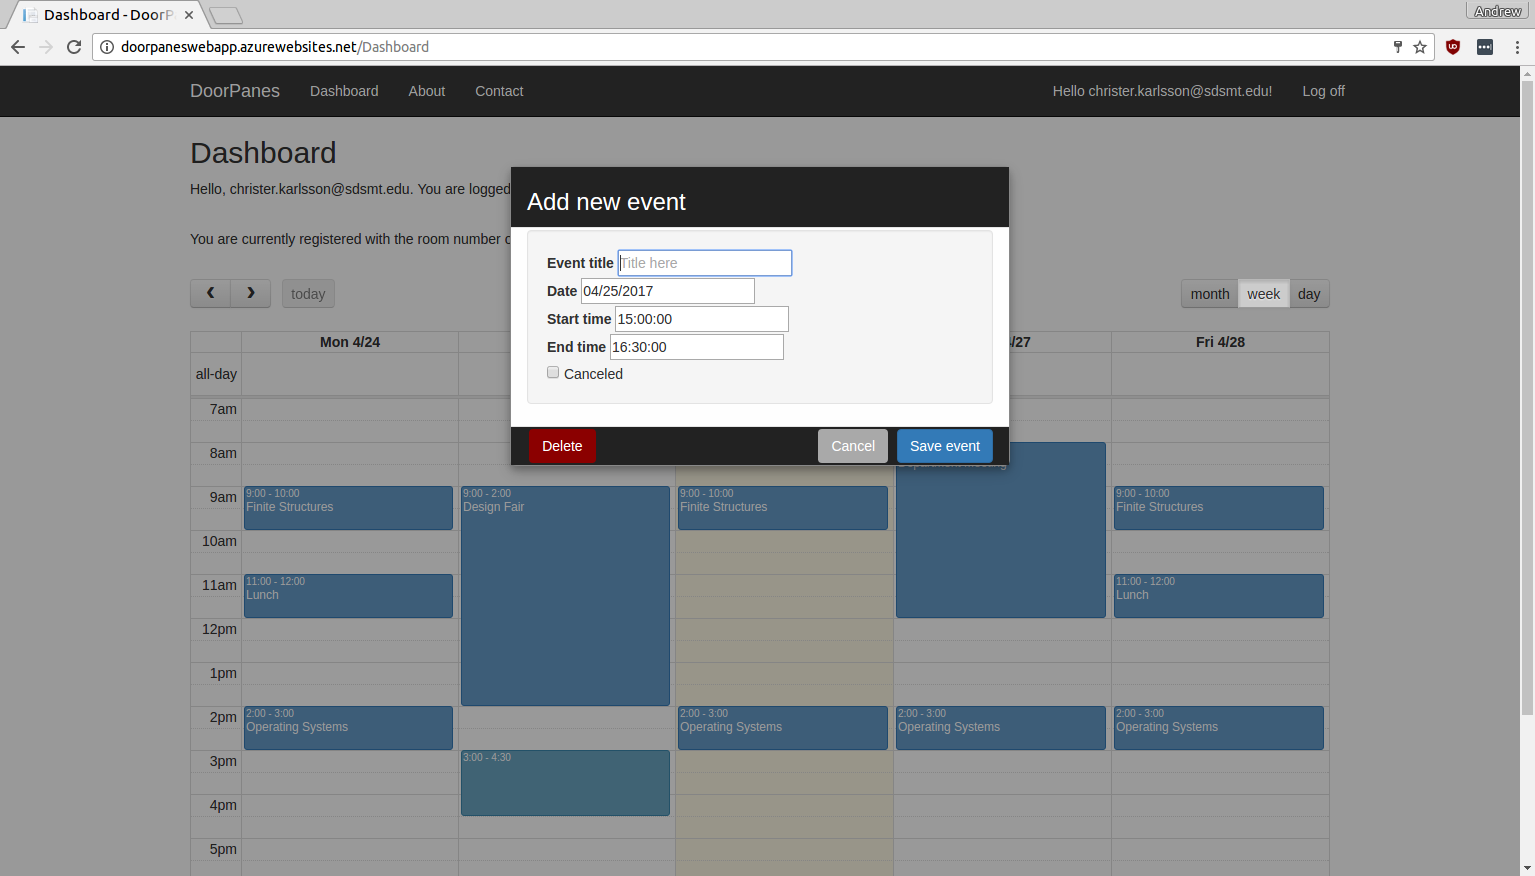
\includegraphics[scale=0.3]{DesignImages/UserGuideImagesWebApp/drag_event.png}
  \caption{Web App Calendar View}
  \label{fig:drag_event}
\end{figure}

\subsection{Web App User Guide} 
% Section Author: Andrew Fagrey
\subsubsection{Navigating to the Web App}
If the web application is live on the web, it can be visited by going to the respective URL. In the case of the development of this project, the URL to go to was www.doorpaneswebapp.azurewebsites.net. Once navigating to the URL in a web browser, the main page will be shown (see the figure below in Figure \ref{fig:main_page}).

Once the Web App is accessible, a user can login to the Web App by clicking the login button in the top left corner, as shown in the figure below (Figure \ref{fig:login_page}).

Once the user has logged in, they will be redirected to the calendar dashboard, where they can add and remove calendar events. This is shown in the figure below (Figure \ref{fig:calendar_view}).


Once a user is viewing the calendar dashboard view, they can add and remove calendar events as they wish. This is shown in Figure \ref{fig:drag_event} .



\subsection{Tablet App User Guide}
Once downloaded, the tablet app will be available for use on Android tablets, preferably using Android 6.0.1.  Details on how to download the app are below.  To use the application, an account must first be made using the web application.  Details about this can be seen above.  

When the app launches, it will ask for log in credentials. Here is where you input your information created on the web application.  The login page can be seen in figure \ref{login} .

\begin{figure}
\centering
  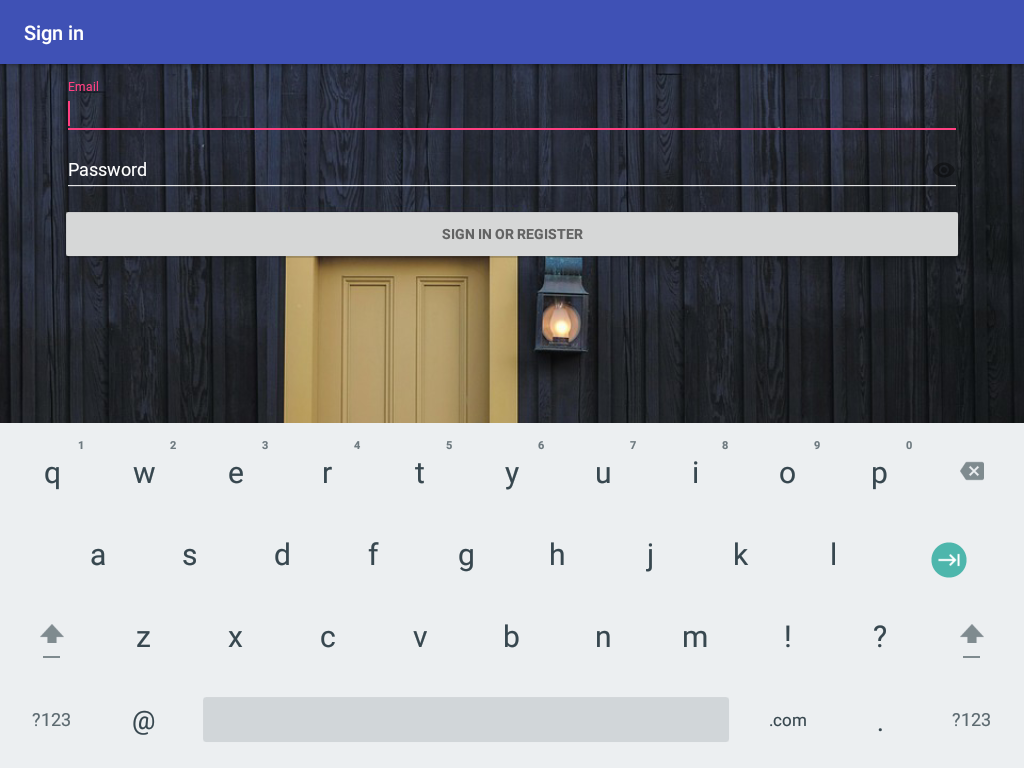
\includegraphics[scale=0.3]{login_final.png}
  \caption{Tablet login page}
  \label{login}
\end{figure}

\begin{figure}
\centering
  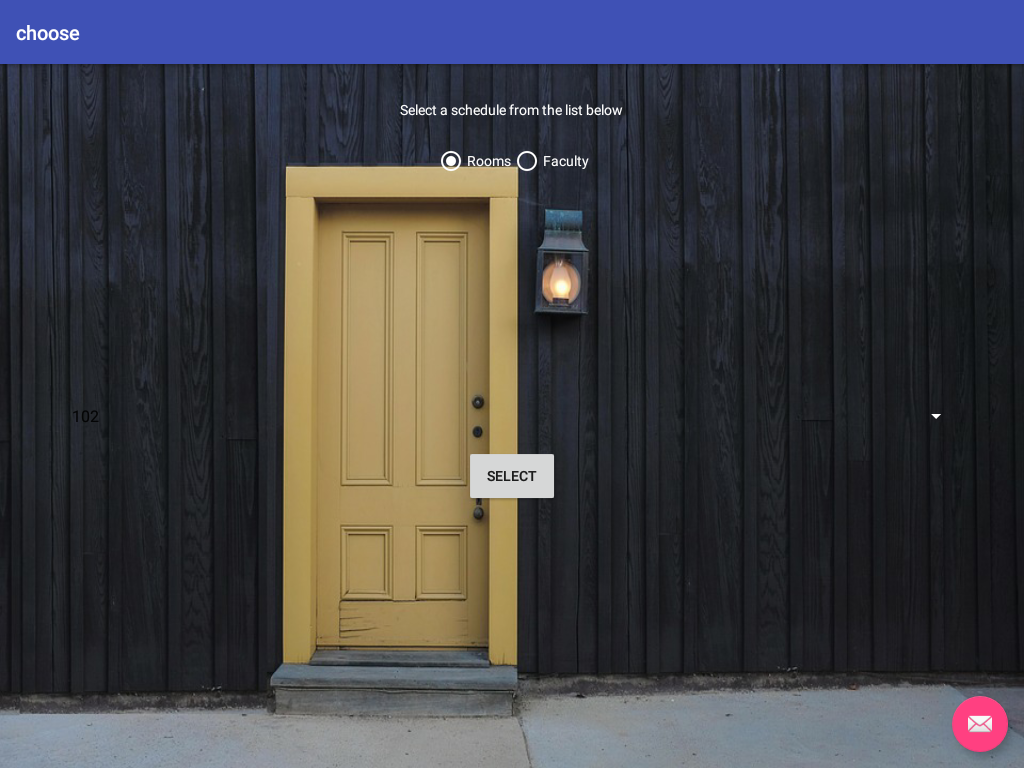
\includegraphics[scale=0.3]{selection_final.png}
  \caption{Tablet calendar selection page}
  \label{selection}
\end{figure}

\begin{figure}
\centering
  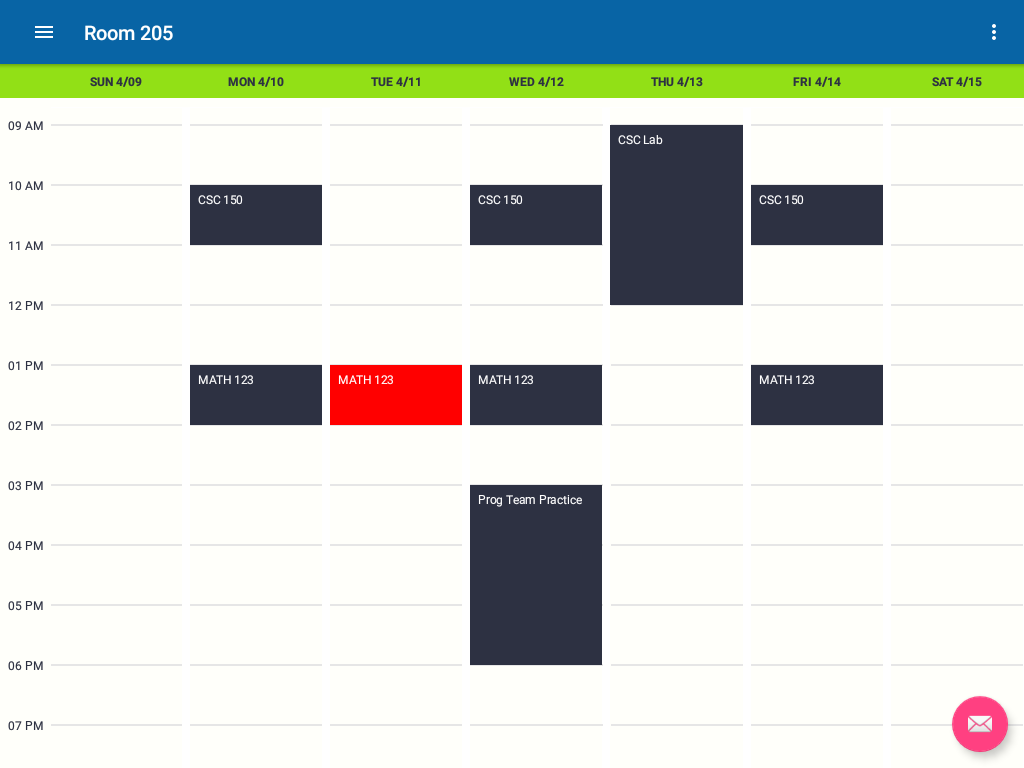
\includegraphics[scale=0.3]{dashboard_final.png}
  \caption{Tablet calendar dashboard}
  \label{dashboard}
\end{figure}

When a user is logged in, Figure \ref{selection} shows the next page that displays a list of available calendars to choose to view.  The radio buttons switch between viewing faculty and room lists.  The dropdown menu shows all the schedules.  Select the schedule you would like to view and press the select button.

When a calendar is selected, the application switches to a different page shown in Figure \ref{dashboard}.  On this page it is important to click the sync button found in the navigation drawer.  Once this button is clicked, the sync process starts and ever 10 seconds a request will be sent to update the events.  Any changes will be updated onto the screen.



On this page all scheduled events will be viewed for that calendar.  To choose a different calendar, simply hit the back button and choose another calendar on the choose page.  








\pagebreak
% Section Author: Andrew Fagrey
\section{Installation Guide}
\subsection{Web App}
The web app is (when uploaded to an Azure service) available as a public website. It can be visited by any computer that has a web browser. There is no need to install any software on your computer to use the web app.

\subsection{Web API}
The web API is not a feature that is available for end users. It is only used by developers to sync data to the tablet app. If you need to use the API, please contact a developer on the project.

\subsection{Tablet App}
The tablet app (once published) would be available from the Google Play store. The process of installing the application would be exactly the same as any other app. A user would visit the Google Play store app on their respective app store and download the app to their tablet that way.
 %% All tracks
% !TEX root = DesignDocument.tex


\chapter{Class Index}
% !TEX encoding = UTF-8 Unicode
% !TEX root = DesignDocument.tex


\section{Class List}
Here are the classes, structs, unions and interfaces with brief descriptions\-:\begin{DoxyCompactList}
\item\contentsline{section}{\hyperlink{class_poly}{Poly} }{\pageref{class_poly}}{}
\end{DoxyCompactList}

\chapter{Class Documentation}
\hypertarget{class_poly}{\section{Poly Class Reference}
\label{class_poly}\index{Poly@{Poly}}
}
\subsection*{Public Member Functions}
\begin{DoxyCompactItemize}
\item 
\hyperlink{class_poly_aa3def076b74bed67904976ad4f9fe9b1}{Poly} ()
\item 
\hyperlink{class_poly_a2f8530284140c31c0aa391dd4d0b61be}{$\sim$\-Poly} ()
\item 
int \hyperlink{class_poly_a14a7ad77ce612b0c54f531d307ee4b39}{myfunction} (int)
\end{DoxyCompactItemize}


\subsection{Constructor \& Destructor Documentation}
\hypertarget{class_poly_aa3def076b74bed67904976ad4f9fe9b1}{\index{Poly@{Poly}!Poly@{Poly}}
\index{Poly@{Poly}!Poly@{Poly}}
\subsubsection[{Poly}]{\setlength{\rightskip}{0pt plus 5cm}Poly\-::\-Poly (
\begin{DoxyParamCaption}
{}
\end{DoxyParamCaption}
)}}\label{class_poly_aa3def076b74bed67904976ad4f9fe9b1}
My constructor \hypertarget{class_poly_a2f8530284140c31c0aa391dd4d0b61be}{\index{Poly@{Poly}!$\sim$\-Poly@{$\sim$\-Poly}}
\index{$\sim$\-Poly@{$\sim$\-Poly}!Poly@{Poly}}
\subsubsection[{$\sim$\-Poly}]{\setlength{\rightskip}{0pt plus 5cm}Poly\-::$\sim$\-Poly (
\begin{DoxyParamCaption}
{}
\end{DoxyParamCaption}
)}}\label{class_poly_a2f8530284140c31c0aa391dd4d0b61be}
My destructor 

\subsection{Member Function Documentation}
\hypertarget{class_poly_a14a7ad77ce612b0c54f531d307ee4b39}{\index{Poly@{Poly}!myfunction@{myfunction}}
\index{myfunction@{myfunction}!Poly@{Poly}}
\subsubsection[{myfunction}]{\setlength{\rightskip}{0pt plus 5cm}int Poly\-::myfunction (
\begin{DoxyParamCaption}
\item[{int}]{a}
\end{DoxyParamCaption}
)}}\label{class_poly_a14a7ad77ce612b0c54f531d307ee4b39}
my own example function fancy new function

new variable 

The documentation for this class was generated from the following file\-:\begin{DoxyCompactItemize}
\item 
hello.\-cpp\end{DoxyCompactItemize}

  %% All tracks
% !TEX encoding = UTF-8 Unicode
% !TEX root = DesignDocument.tex

\chapter{Business Plan}



\section{Business Model}

\section{Market and Competition}

\section{Regulatory environment}

\section{Intellectual Property and Freedom to Operate}

\section{Management Team and Advisors}

\section{Sources and Uses of Capital}

\section{Financial Statements}

\section{Metrics and Milestones}

\section{Exit Plan}

   %% Entrepreneur track only 
% !TEX root = DesignDocument.tex


\chapter{Experimental Log}

For research projects one needs to keep a log of all research/lab activities.   

%% If you have multiple labs, you may want to break the labs into sections, check 
%% with the profession on format.
%% \section{Lab 1}

\begin{description}
\item [10/15/15]  Ran modified filter on data sets 1 - 6.  Results were ...
\item [10/17/15]  Changed tolerance on sensor and collected data.  These ...
\end{description}   %% Research track  only
% !TEX root = DesignDocument.tex


\chapter{Research Results}

This chapter describes the results and conclusions of your research.   This would be the final report for a research project.  

\section{Result 1}

\section{Result 2}

\section{Conclusions}

\section{Further work}    %% Research track  only

\bibliographystyle{plain}
\bibliography{designrefs.bib}
\addcontentsline{toc}{chapter}{Bibliography}


% We want to add the Software agreement to the end and number the
% pages separately from the document.  We don't want to do a standard
% chapter heading, but we do want it to appear in the table of contents
% and in the index used for on-line viewing.  We defined the \agreement
% macro to set things up for us.
\agreement

\chapter{Software Agreement}
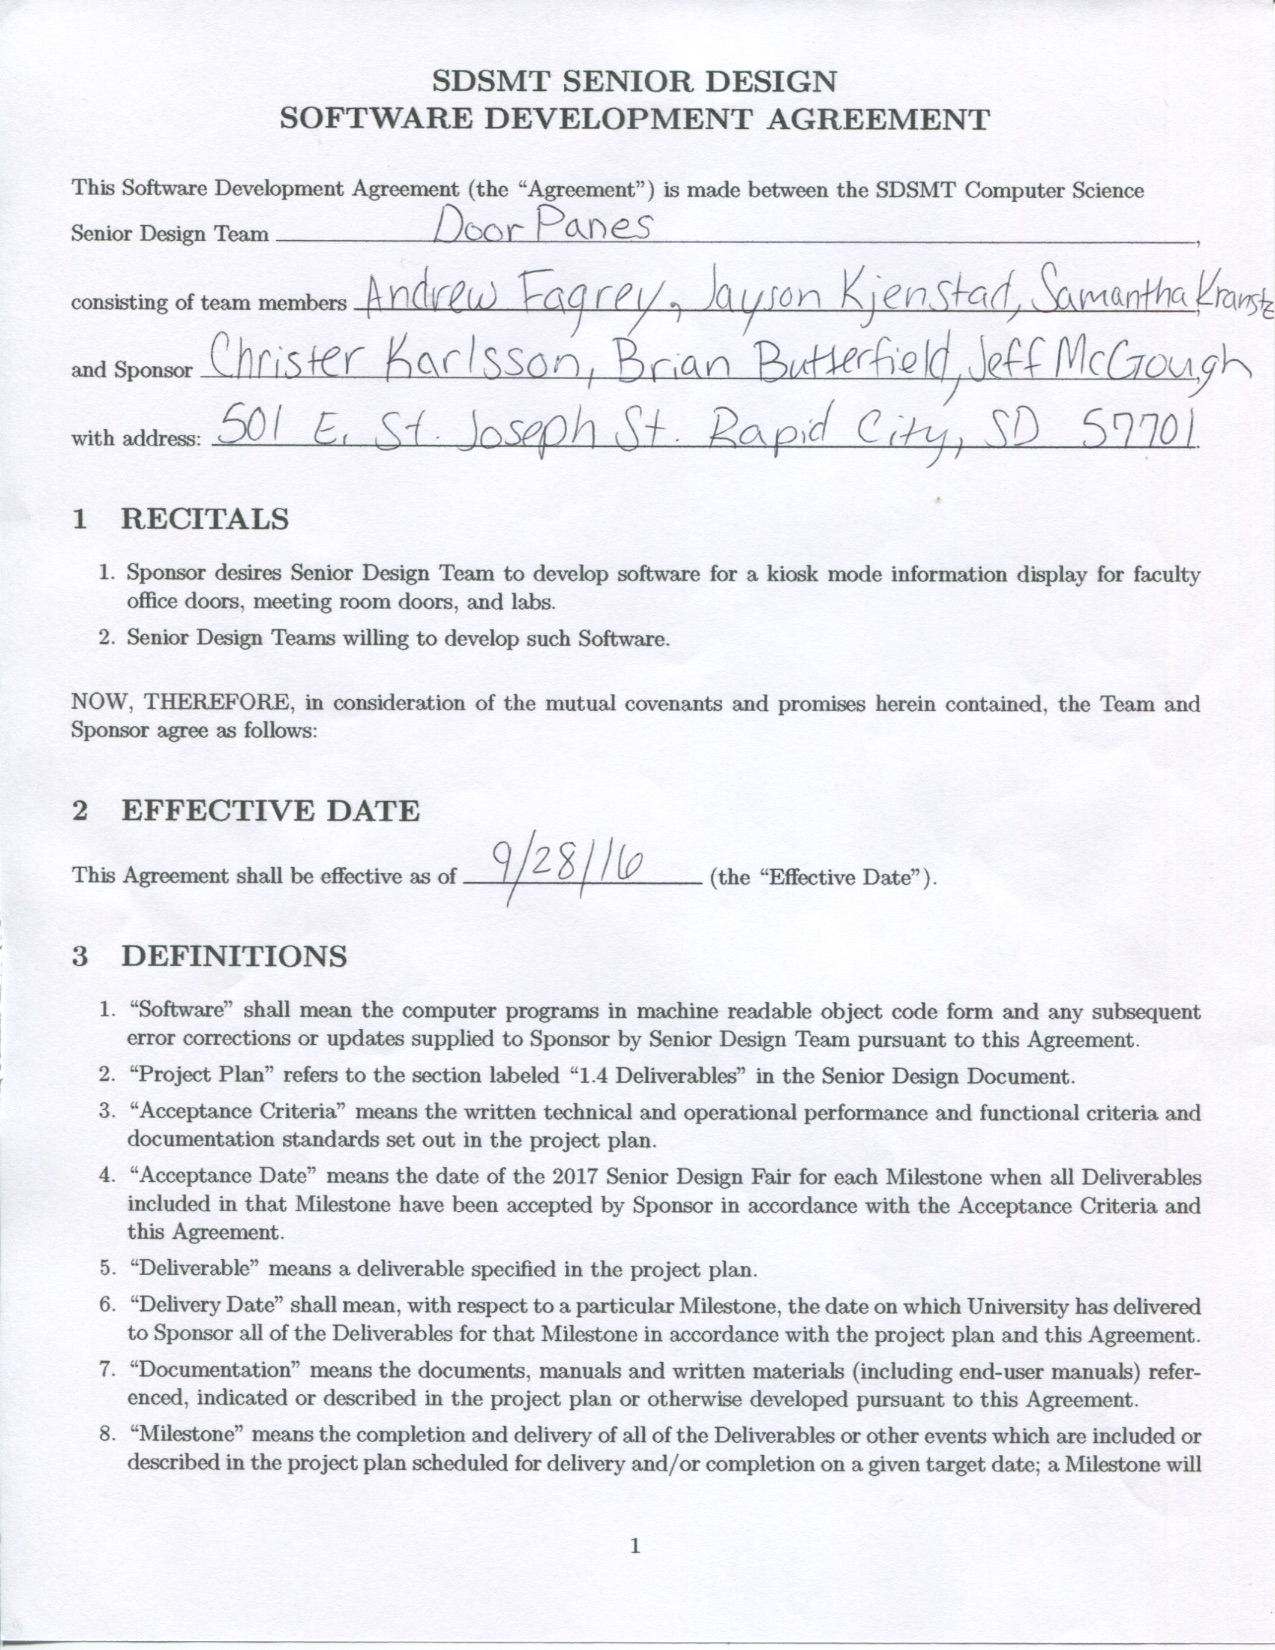
\includepdf[pages={1-5}]{SoftwareContract.pdf}

% In our style file, appendices are numbered with capital letters
\appendix

\chapter{Product Description}


Write a description of the product to be developed.
Use sectioning commands as neccessary.
\vspace{2\baselineskip}

\centerline{\Large {\bf NOTE:} {\em This is part of the contract.}}



\chapter{Publications}   %% Research track 
% !TEX root = DesignDocument.tex


Research Track:  
This chapter will include any publications generated from the research.  Most likely these will be preprints and one will just include the pdf.

%\includepdf[pages={1-5}]{Pub1.pdf}



\chapter{Sprint Reports}
% !TEX root = DesignDocument.tex


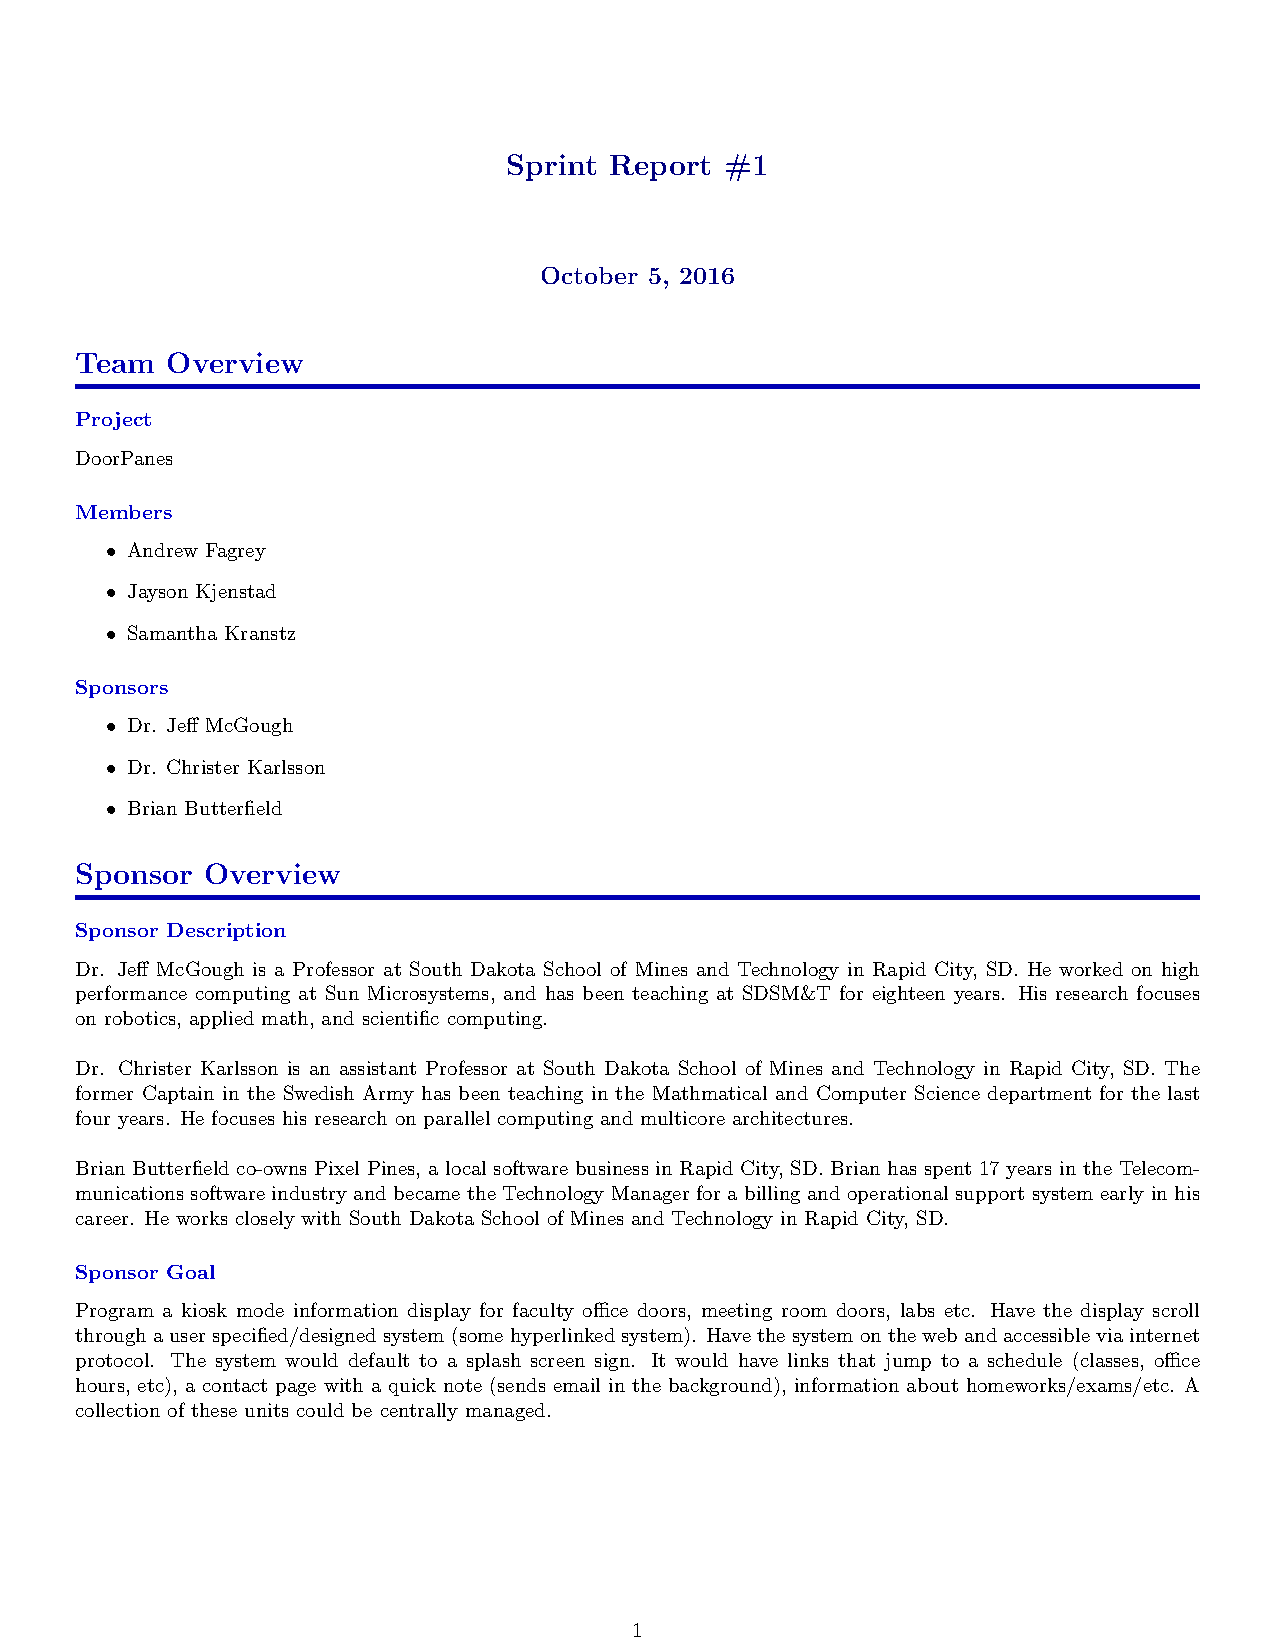
\includepdf[pages=-]{SprintReport1.pdf}

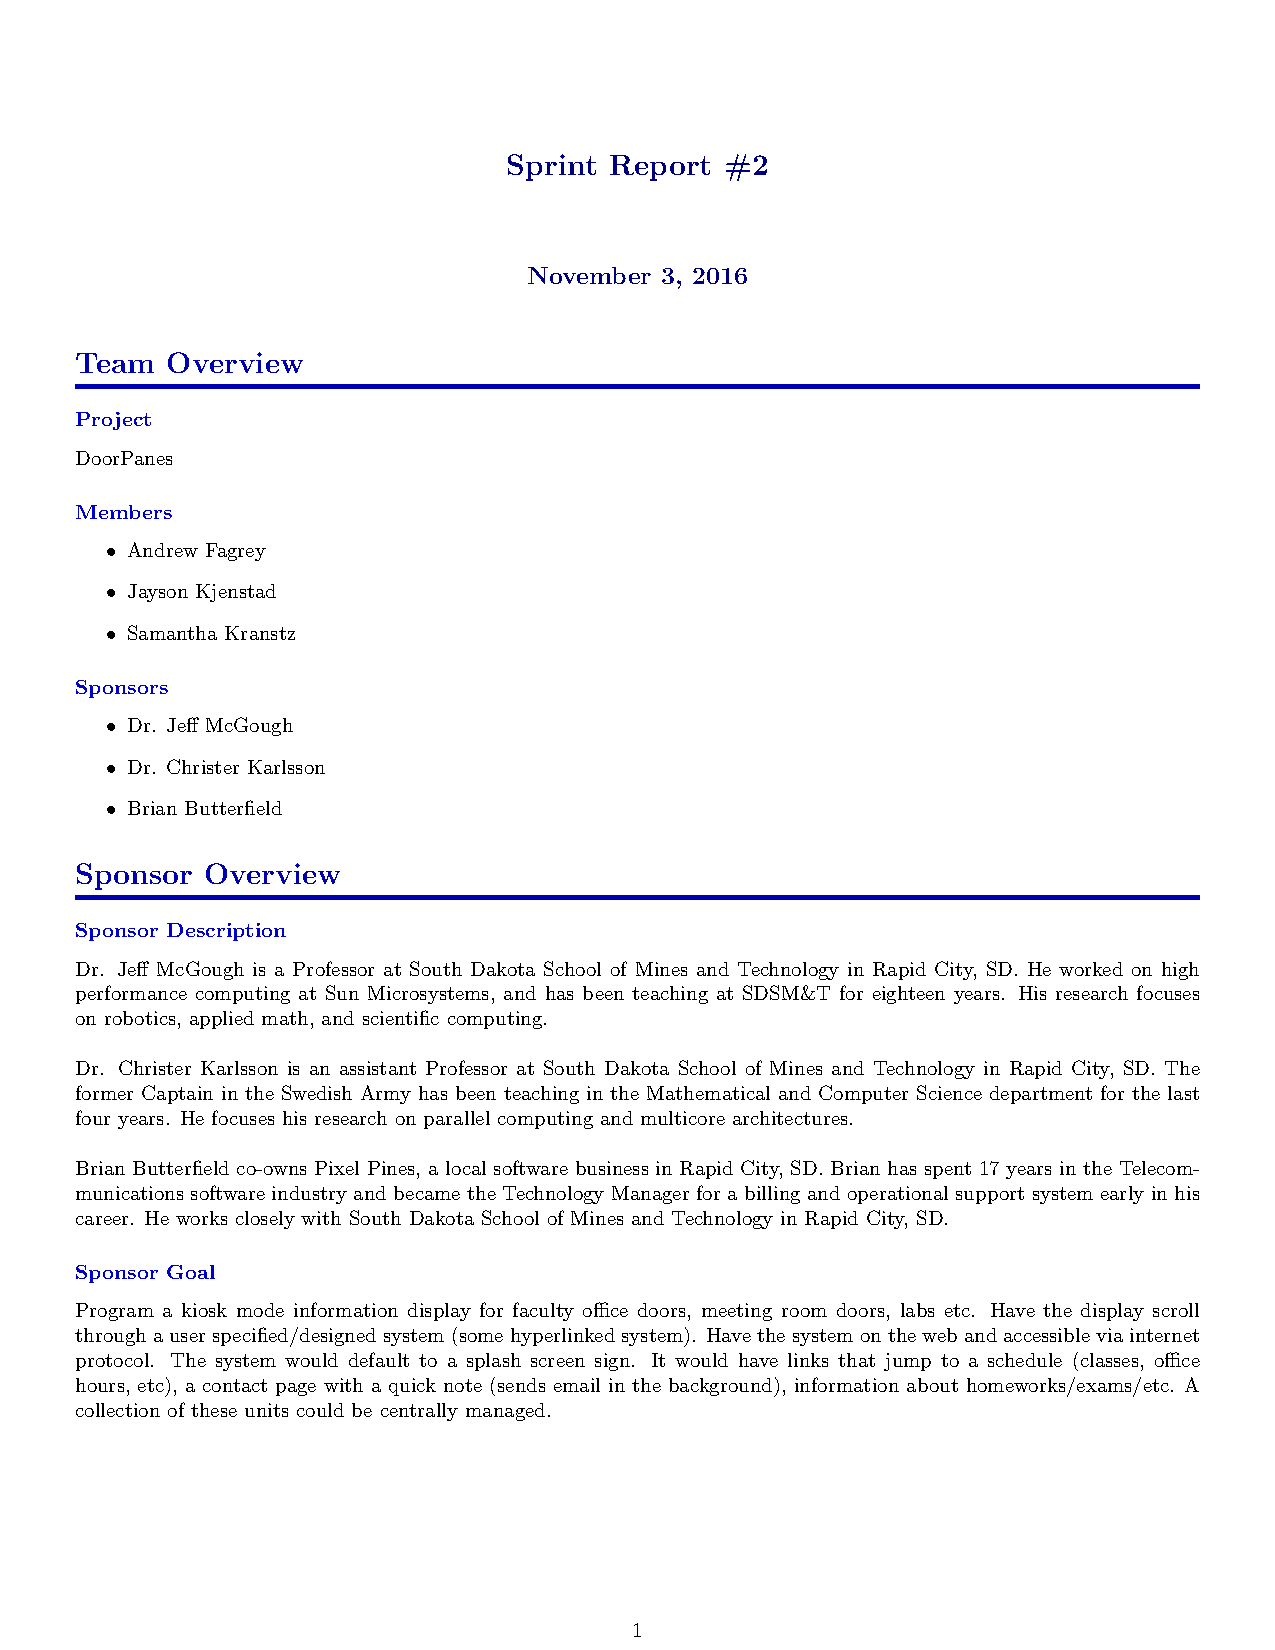
\includepdf[pages=-]{SprintReport2.pdf}

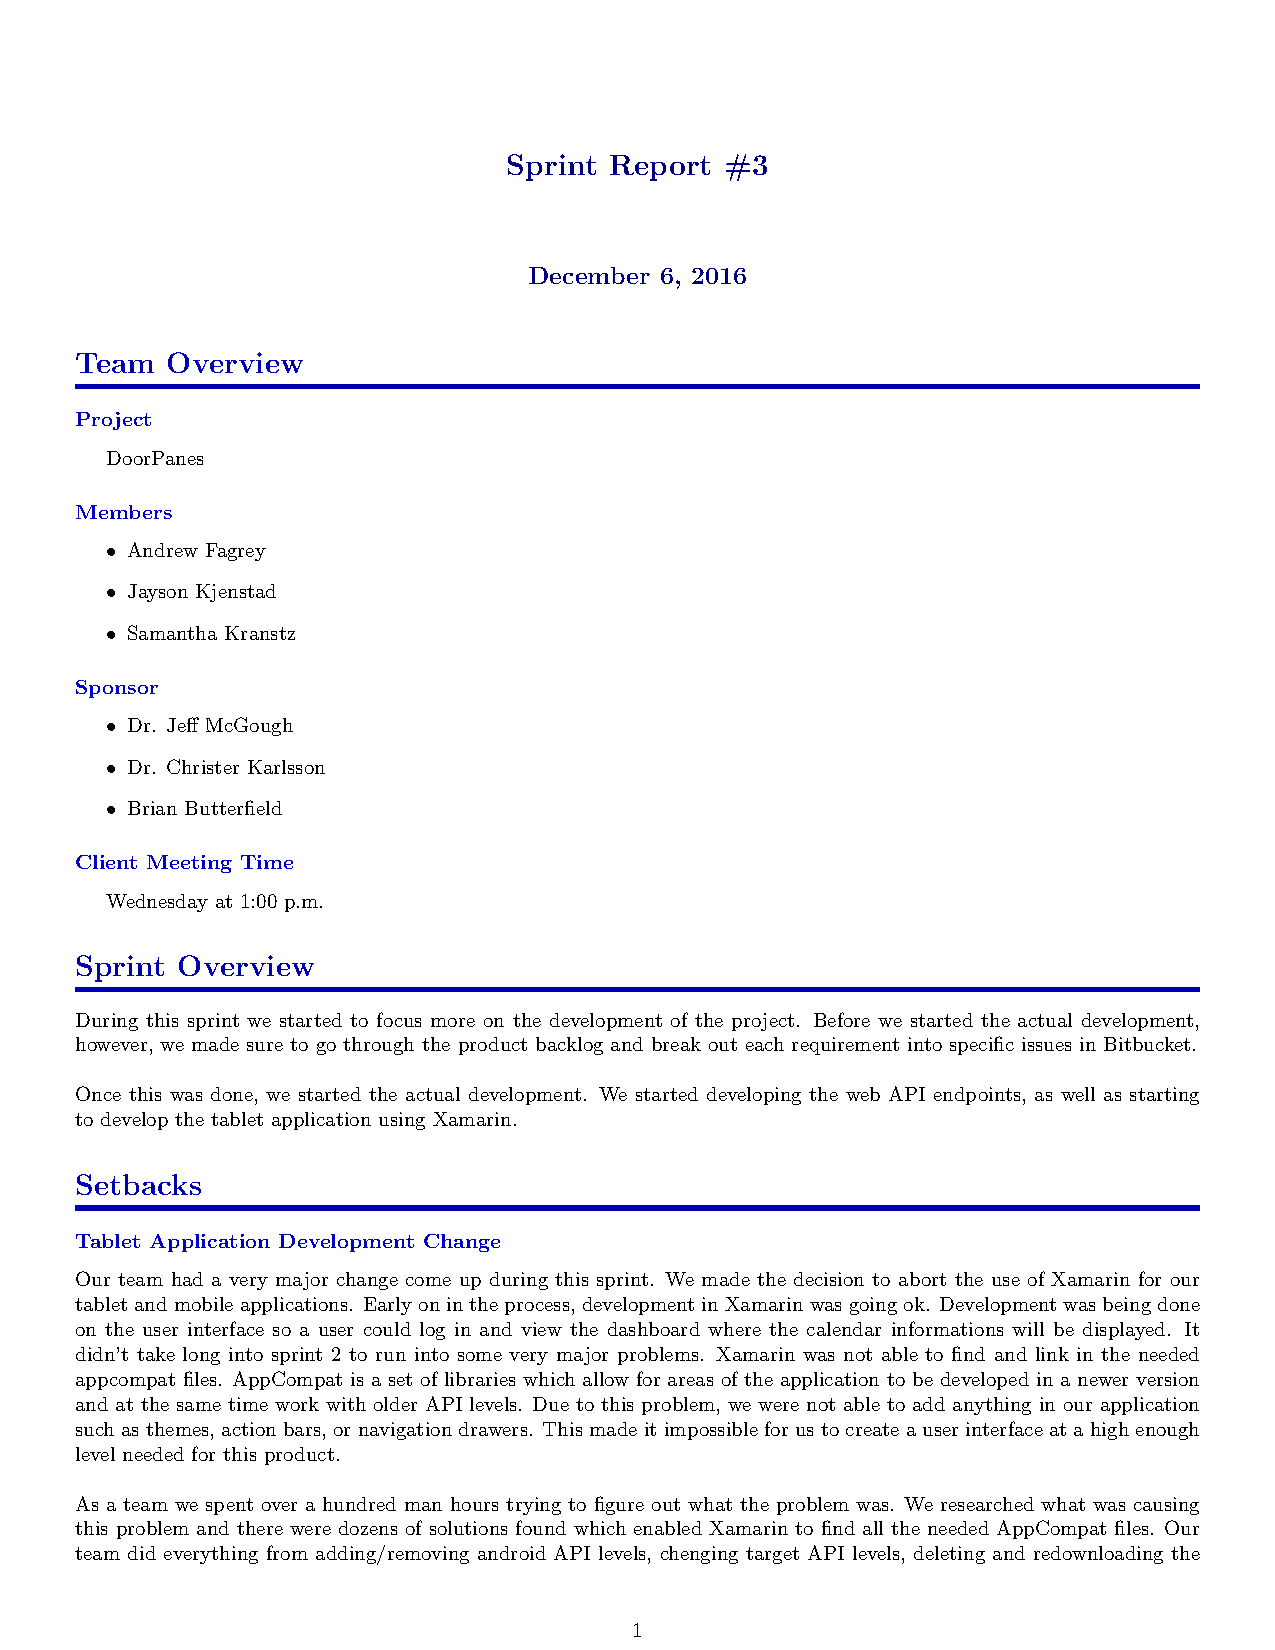
\includepdf[pages=-]{SprintReport3.pdf}

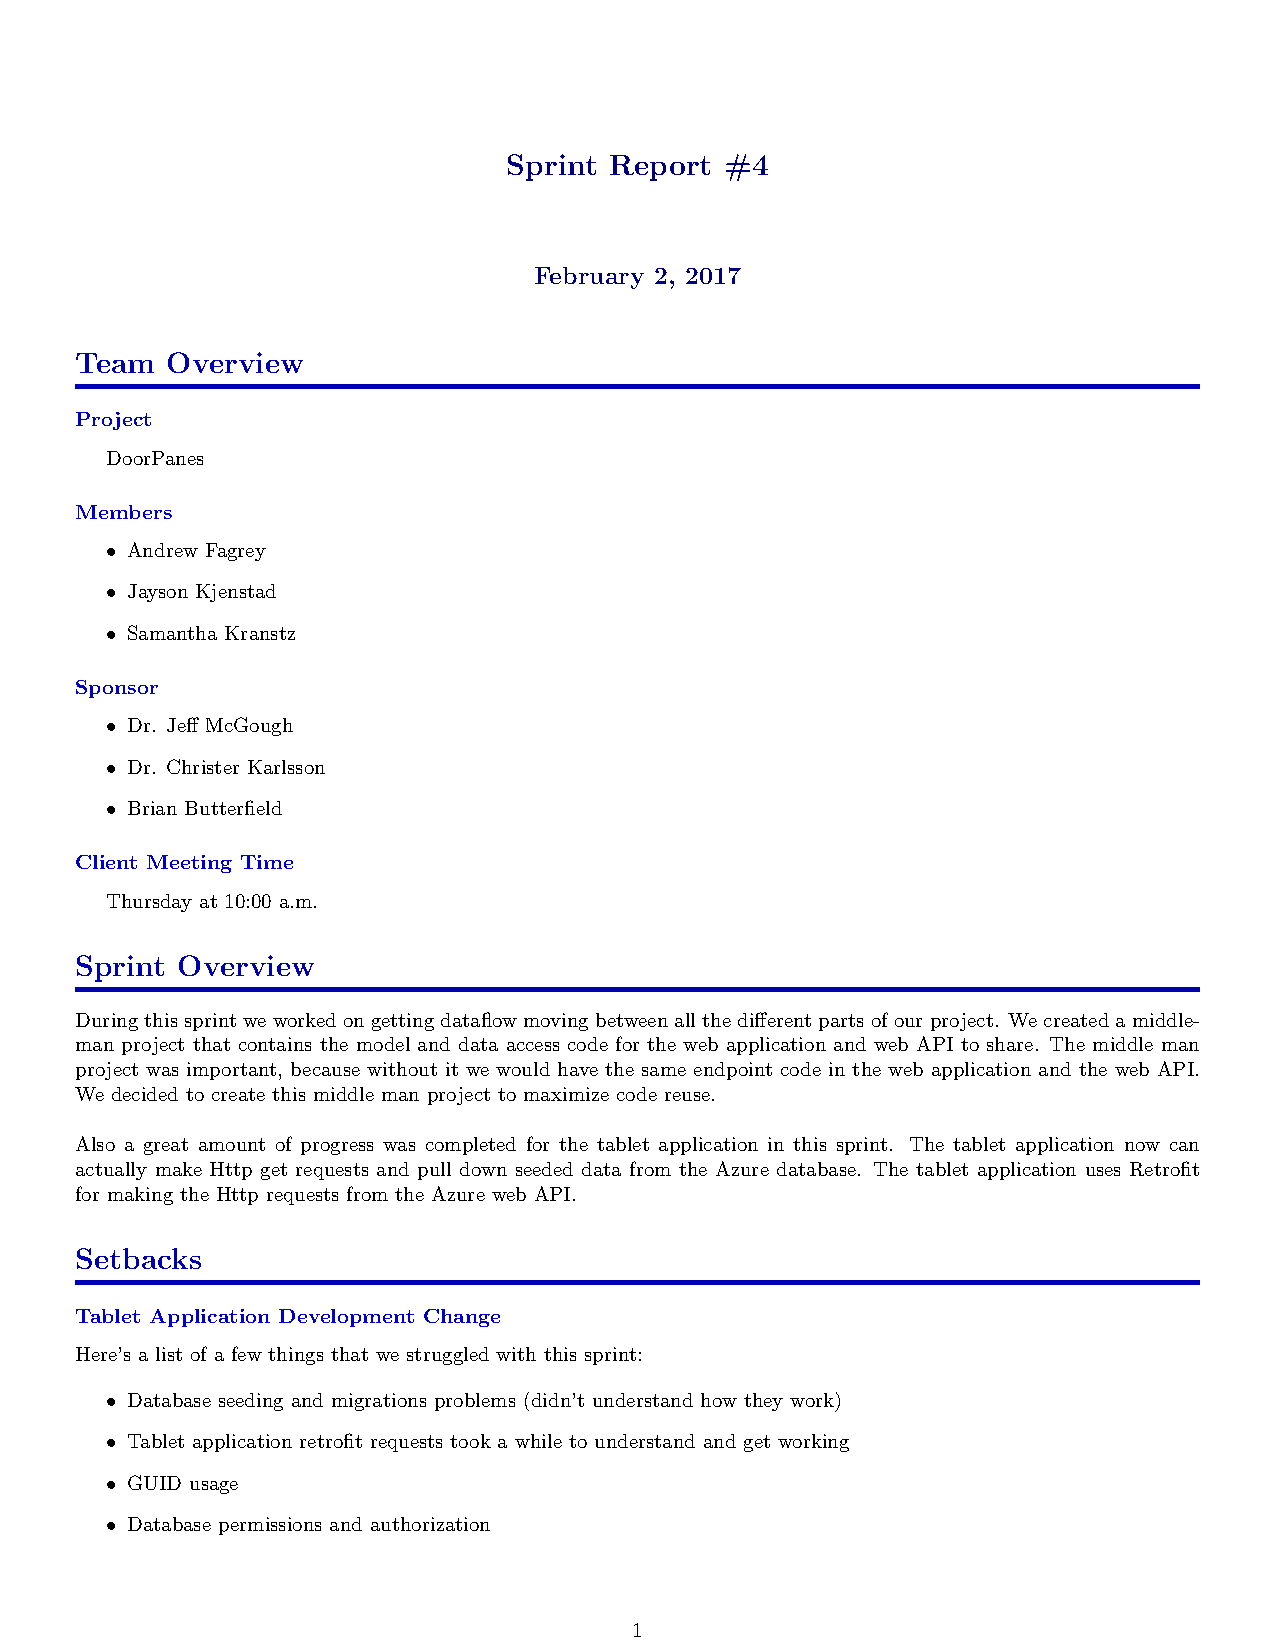
\includepdf[pages=-]{SprintReport4.pdf}

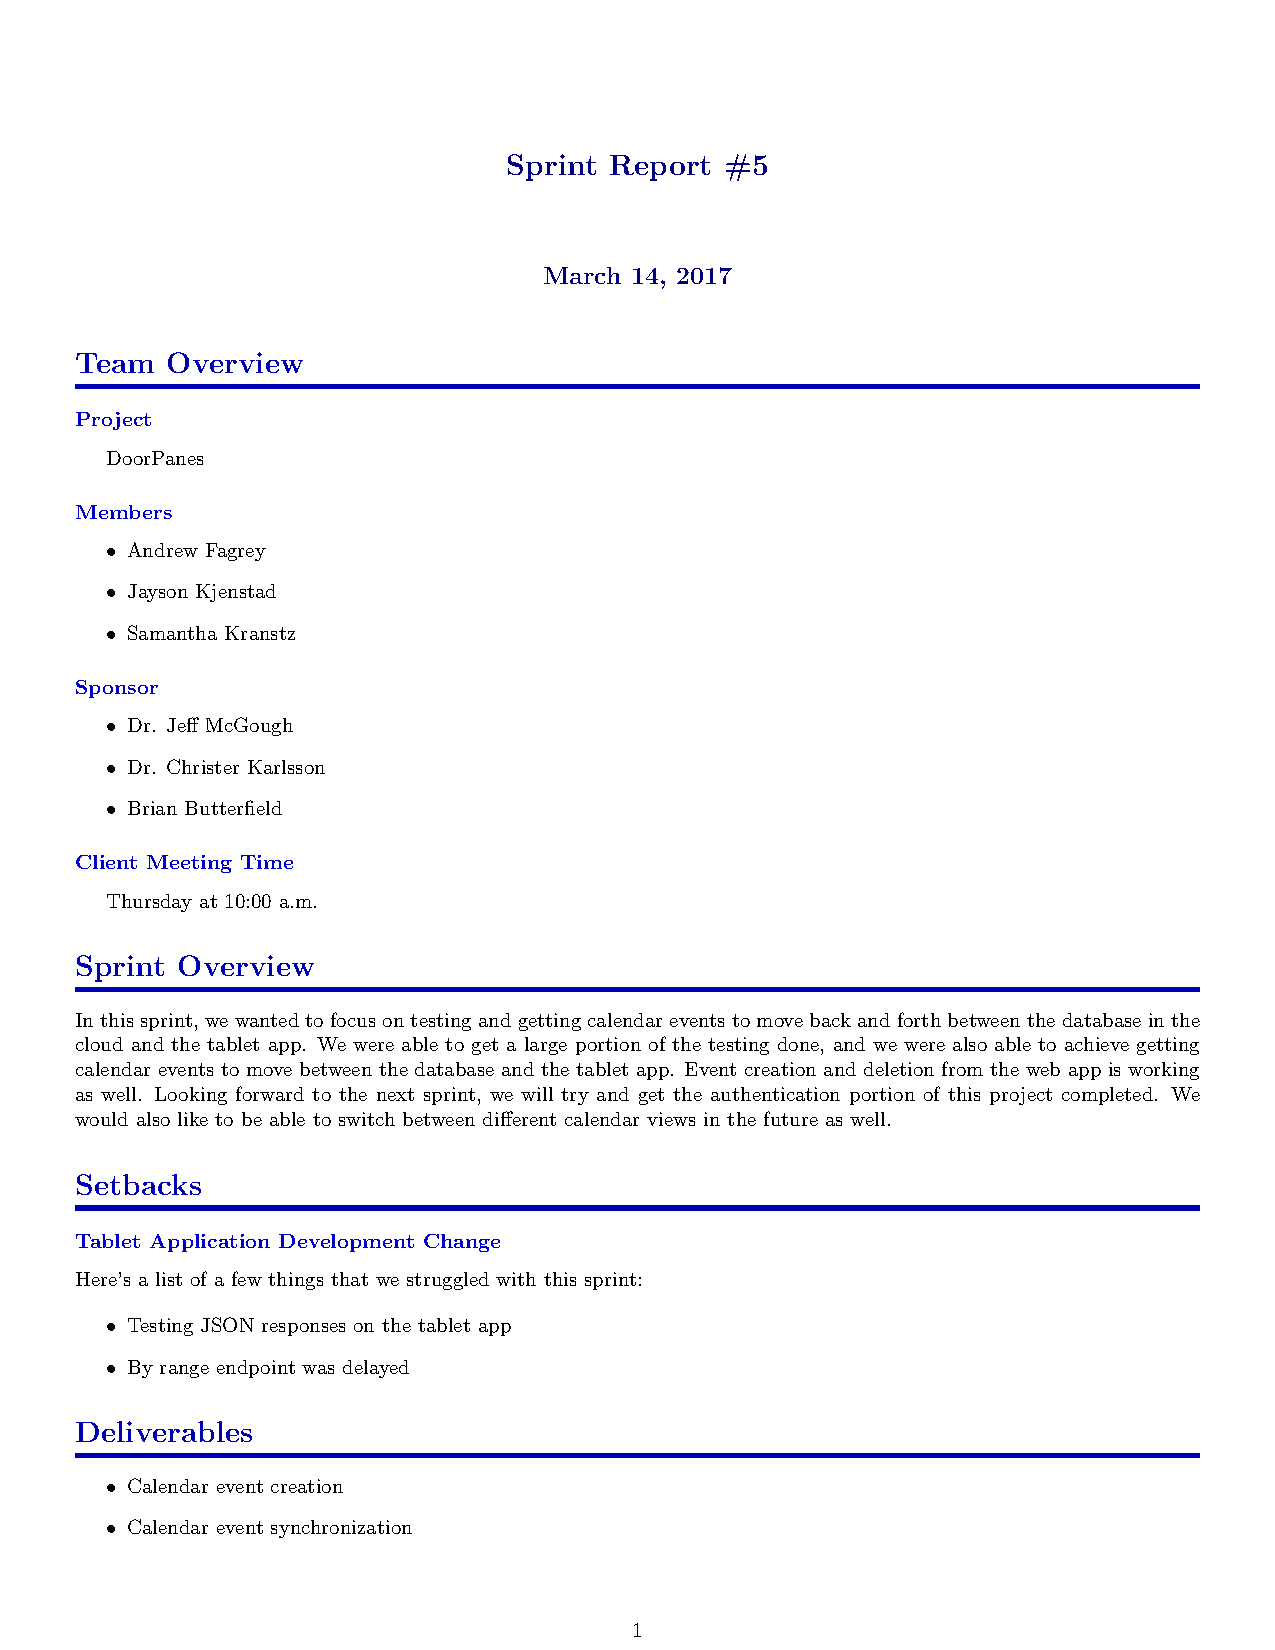
\includepdf[pages=-]{SprintReport5.pdf}

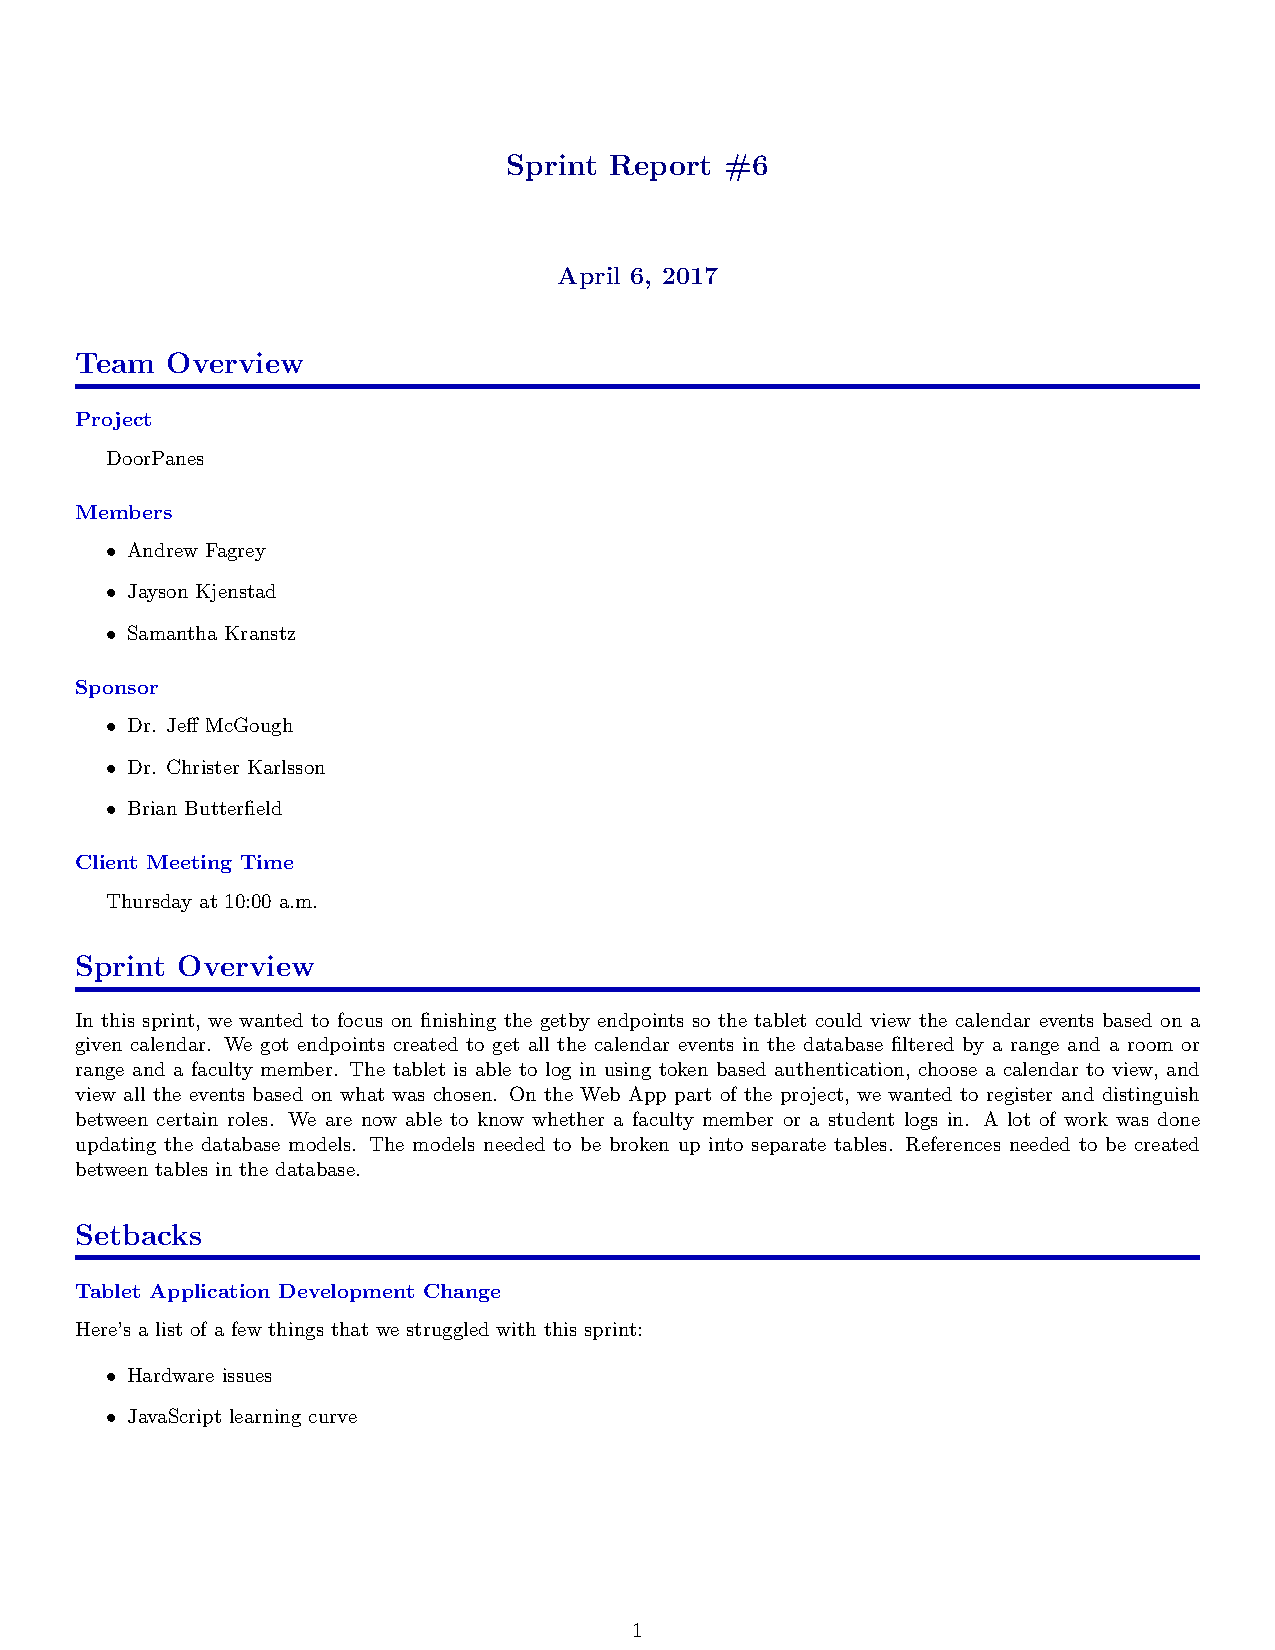
\includepdf[pages=-]{SprintReport6.pdf}

\chapter{Industrial Experience and Resumes}
% !TEX root = DesignDocument.tex



\section{Resumes}

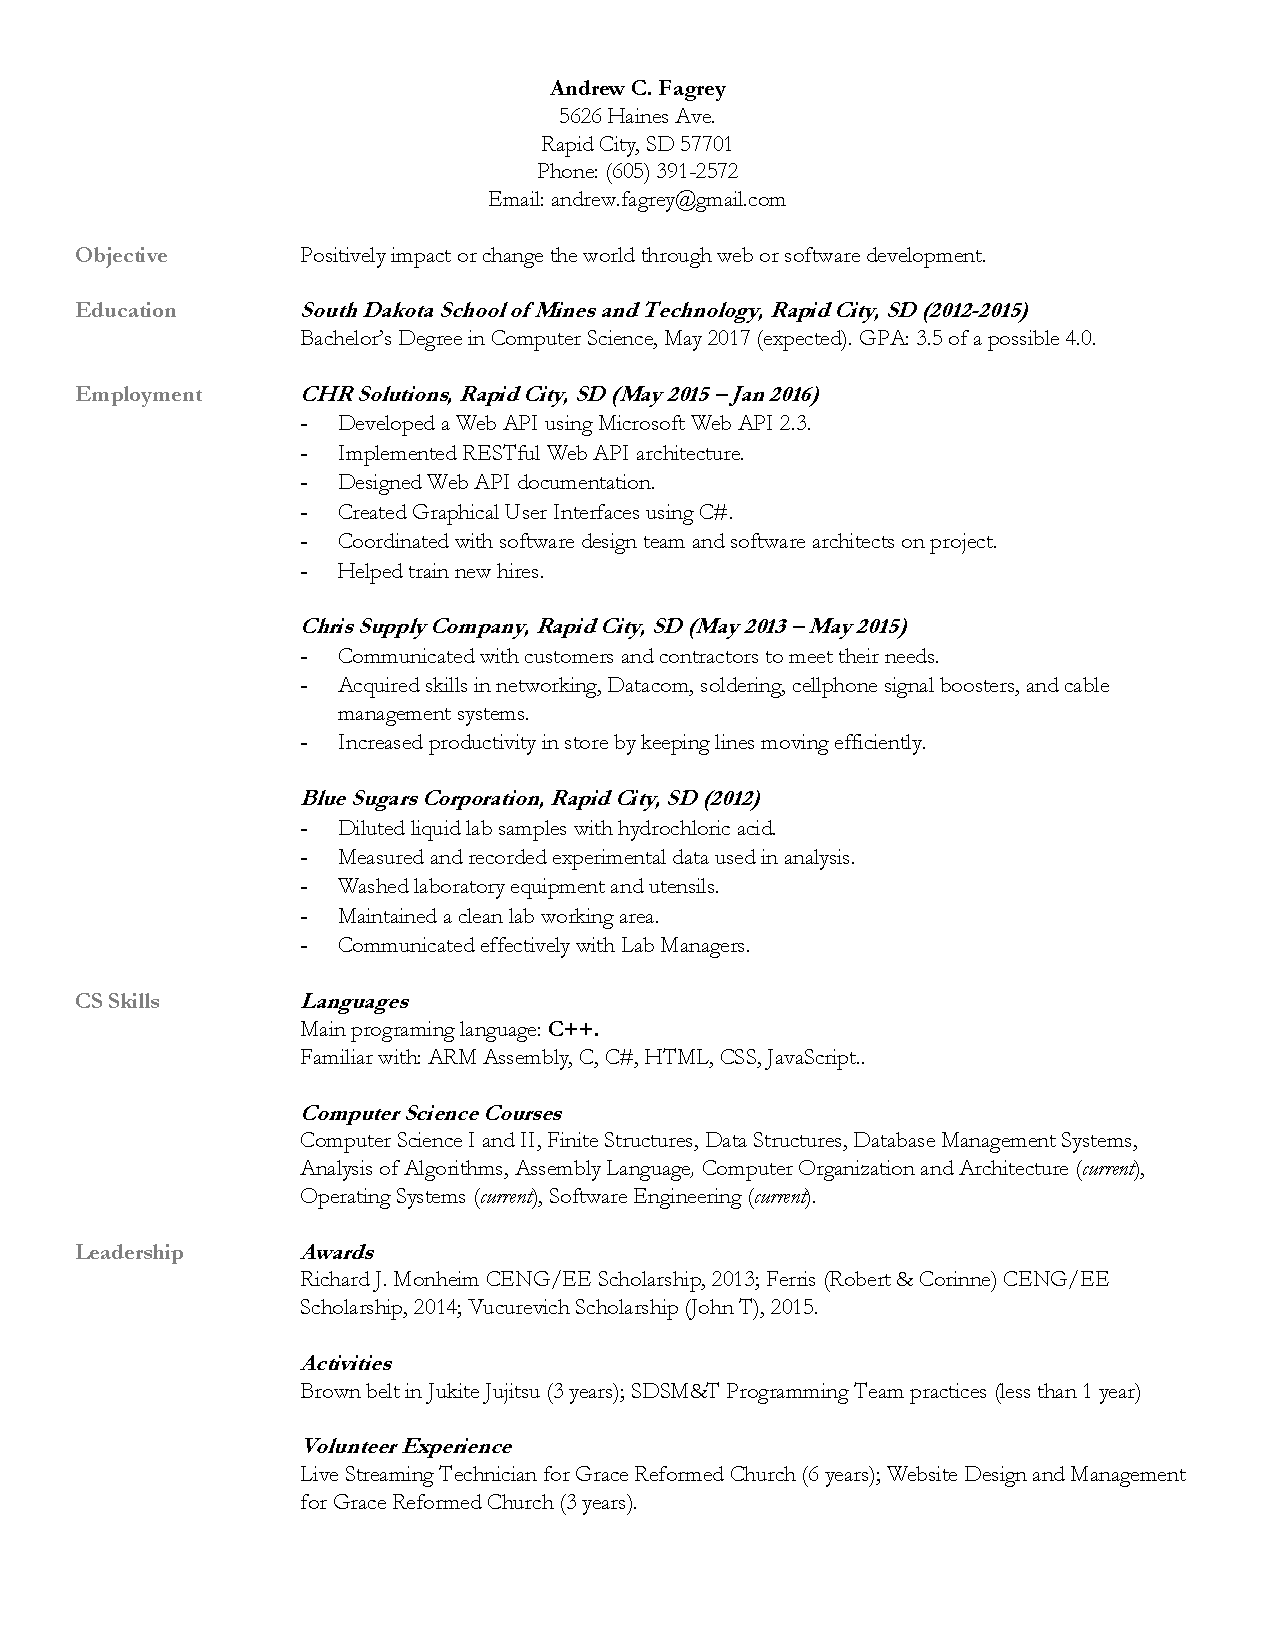
\includepdf{andrew_fagrey_resume_2016.pdf}


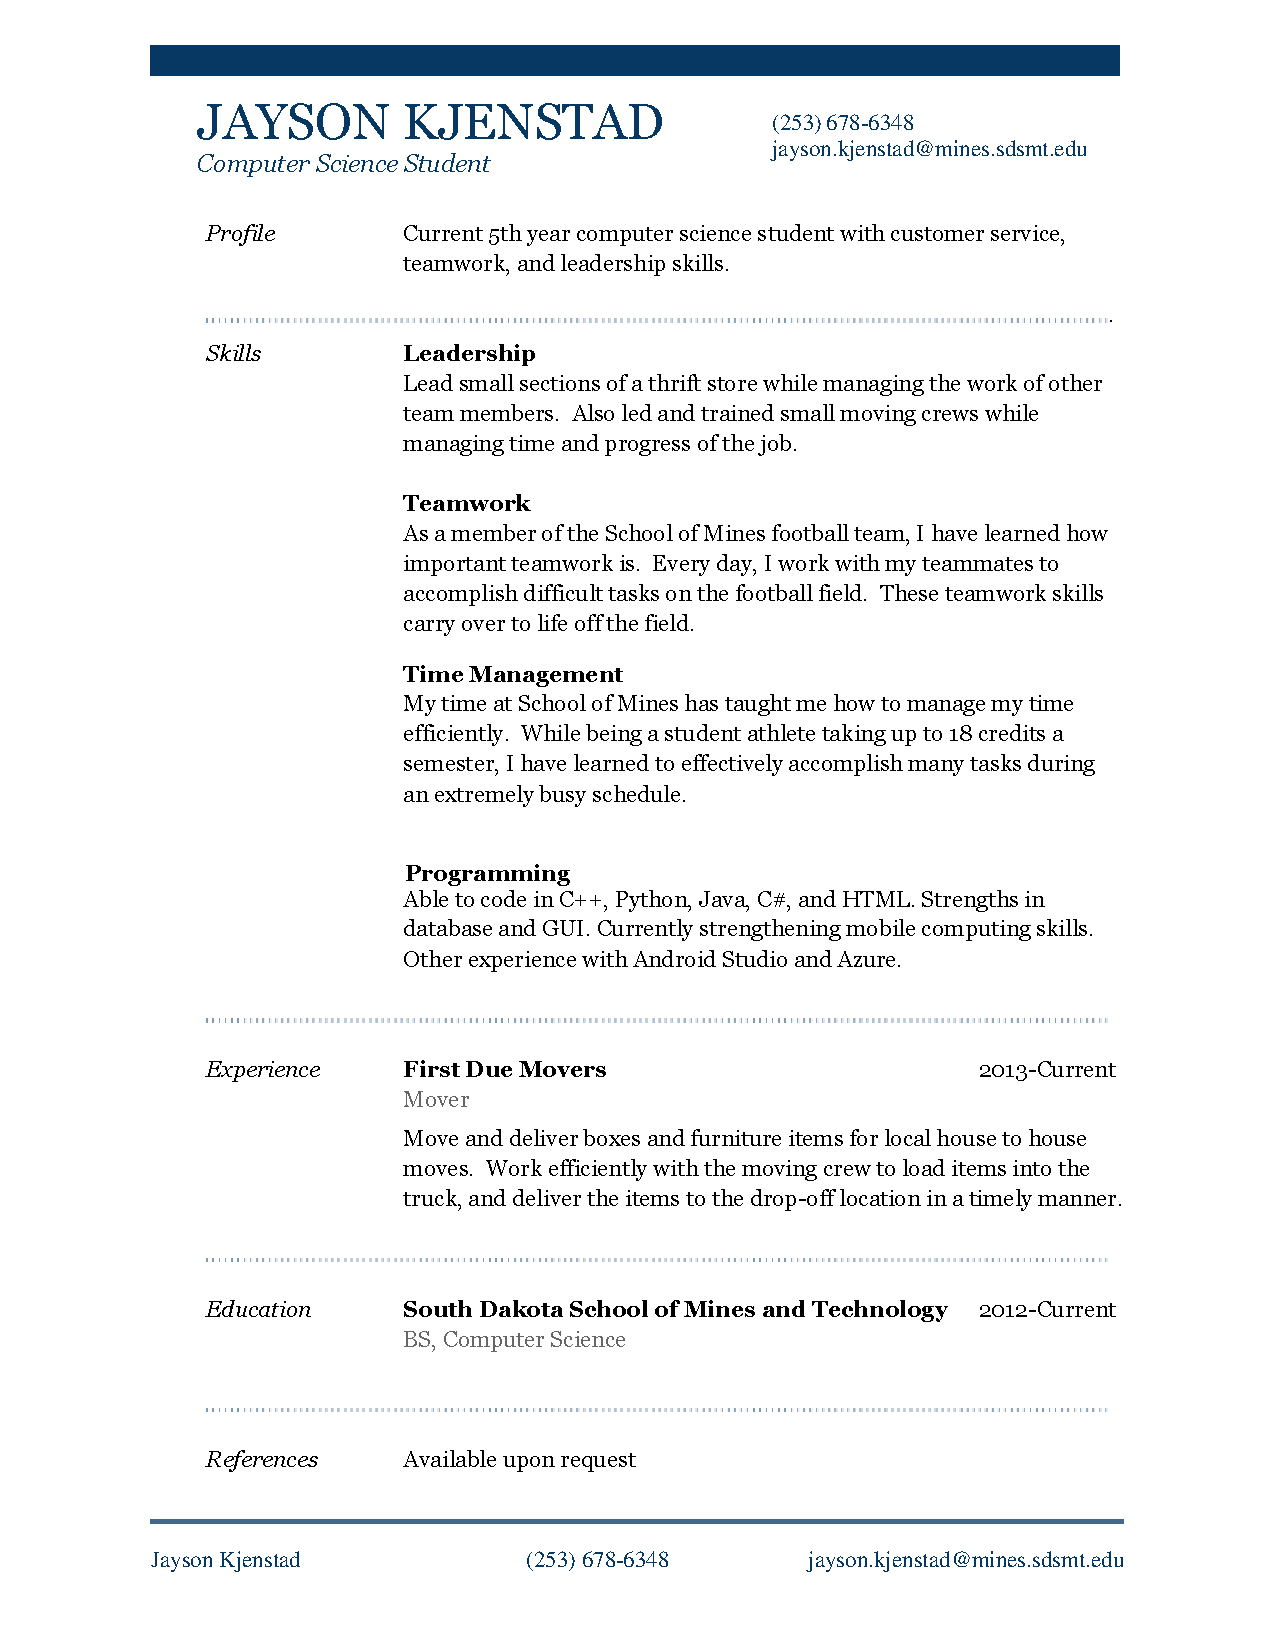
\includepdf{Resume_Jayson.pdf}



\includepdf{skranstzresume.pdf}




\chapter{Acknowledgment}
\label{SpecialThanks}  
Thanks  

\chapter{Supporting Materials}

This document will contain several appendices used as a way to separate out major 
component details, logic details, or tables of information.  Use of this structure 
will help keep the document clean, readable, and organized. 



% chapters in backmatter don't have numbers, but they appear in the
% table of contents, and are numbered BM-X where X is the page number
% relative to where the backmatter begins.
\backmatter

%% Example
%\chapter{Course Syllabus}
%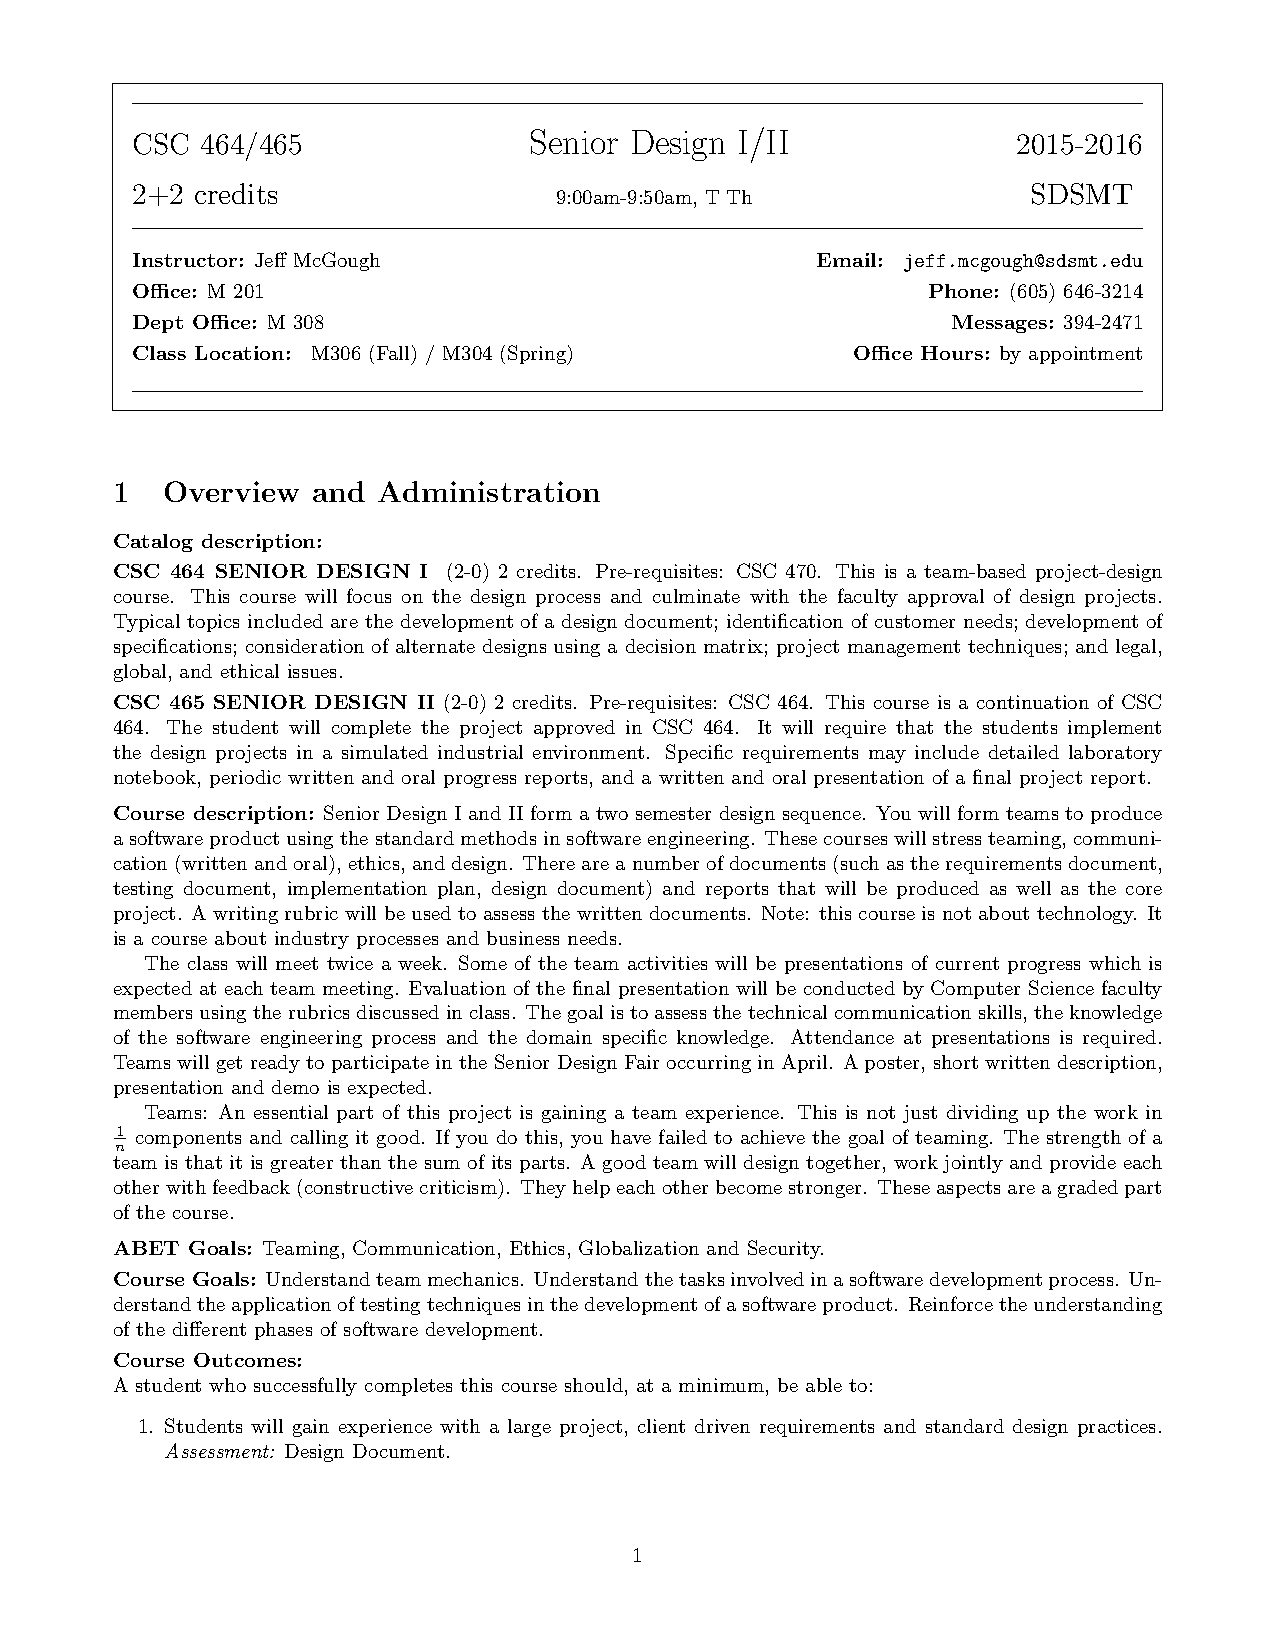
\includepdf[pages={1-17}]{syllabus.pdf}

%%% Remove after reading
\chapter{\LaTeX\ Example}
% !TEX root = DesignDocument.tex


\LaTeX\xspace sample file:  {\color{red} Remove from submitted materials}

\section{Introduction}
This is a sample input file.  Comparing it with the output it
generates can show you how to produce a simple document of
your own.

\section{Ordinary Text}  % Produces section heading.  Lower-level
                                    % sections are begun with similar 
                                    % \subsection and \subsubsection commands.

The ends  of words and sentences are marked 
  by   spaces. It  doesn't matter how many 
spaces    you type; one is as good as 100.  The
end of   a line counts as a space.

One   or more   blank lines denote the  end 
of  a paragraph.  

Since any number of consecutive spaces are treated like a single
one, the formatting of the input file makes no difference to
      \TeX,         % The \TeX command generates the TeX logo.
but it makes a difference to you.  
When you use
      \LaTeX,       % The \LaTeX command generates the LaTeX logo.
making your input file as easy to read as possible
will be a great help as you write your document and when you
change it.  This sample file shows how you can add comments to
your own input file.

Because printing is different from typewriting, there are a 
number of things that you have to do differently when preparing 
an input file than if you were just typing the document directly.  
Quotation marks like 
       ``this'' 
have to be handled specially, as do quotes within quotes: 
       ``\,`this'                  % \, separates the double and single quote.
        is what I just 
        wrote, not  `that'\,''.  

Dashes come in three sizes: an 
       intra-word 
dash, a medium dash for number ranges like 
       1--2, 
and a punctuation 
       dash---like 
this.

A sentence-ending space should be larger than the space between words
within a sentence.  You sometimes have to type special commands in
conjunction with punctuation characters to get this right, as in the
following sentence.
       Gnats, gnus, etc.\    % `\ ' makes an inter-word space.
       all begin with G\@.   % \@ marks end-of-sentence punctuation.
You should check the spaces after periods when reading your output to
make sure you haven't forgotten any special cases.
Generating an ellipsis 
       \ldots\    % `\ ' needed because TeX ignores spaces after 
                  % command names like \ldots made from \ + letters.
                  %
                  % Note how a `%' character causes TeX to ignore the 
                  % end of the input line, so these blank lines do not
                  % start a new paragraph.
with the right spacing around the periods 
requires a special  command.  

\TeX\ interprets some common characters as commands, so you must type
special commands to generate them.  These characters include the
following: 
       \$ \& \% \# \{ and \}.

In printing, text is emphasized by using an
       {\em italic\/}  % The \/ command produces the tiny extra space that
                       % should be added between a slanted and a following
                       % unslanted letter.
type style.  

\begin{em}
   A long segment of text can also be emphasized in this way.  Text within
   such a segment given additional emphasis 
          with\/ {\em Roman} 
   type.  Italic type loses its ability to emphasize and become simply
   distracting when used excessively.  
\end{em}

It is sometimes necessary to prevent \TeX\ from breaking a line where
it might otherwise do so.  This may be at a space, as between the
``Mr.'' and ``Jones'' in
       ``Mr.~Jones'',        % ~ produces an unbreakable interword space.
or within a word---especially when the word is a symbol like
       \mbox{\em itemnum\/} 
that makes little sense when hyphenated across 
       lines.

Footnotes\footnote{This is an example of a footnote.}
pose no problem.

\TeX\ is good at typesetting mathematical formulas like
       \( x-3y = 7 \) 
or
       \( a_{1} > x^{2n} / y^{2n} > x' \).
Remember that a letter like
       $x$        % $ ... $  and  \( ... \)  are equivalent
is a formula when it denotes a mathematical symbol, and should
be treated as one.

\section{Displayed Text}

Text is displayed by indenting it from the left margin.
Quotations are commonly displayed.  There are short quotations
\begin{quote}
   This is a short a quotation.  It consists of a 
   single paragraph of text.  There is no paragraph
   indentation.
\end{quote}
and longer ones.
\begin{quotation}
   This is a longer quotation.  It consists of two paragraphs
   of text.  The beginning of each paragraph is indicated
   by an extra indentation.

   This is the second paragraph of the quotation.  It is just
   as dull as the first paragraph.
\end{quotation}
Another frequently-displayed structure is a list.
The following is an example of an {\em itemized} list.
\begin{itemize}
   \item  This is the first item of an itemized list.  Each item 
          in the list is marked with a ``tick''.  The document
          style determines what kind of tick mark is used.

   \item  This is the second item of the list.  It contains another
          list nested inside it.  The inner list is an {\em enumerated}
          list.
          \begin{enumerate}
              \item This is the first item of an enumerated list that
                    is nested within the itemized list.

              \item This is the second item of the inner list.  \LaTeX\
                    allows you to nest lists deeper than you really should.
          \end{enumerate}
          This is the rest of the second item of the outer list.  It
          is no more interesting than any other part of the item.
   \item  This is the third item of the list.
\end{itemize}
You can even display poetry.
\begin{verse}
   There is an environment for verse \\    % The \\ command separates lines
   Whose features some poets will curse.   % within a stanza.

                           % One or more blank lines separate stanzas.

   For instead of making\\
   Them do {\em all\/} line breaking, \\
   It allows them to put too many words on a line when they'd 
   rather be forced to be terse.
\end{verse}

Mathematical formulas may also be displayed.  A displayed formula is
one-line long; multi-line formulas require special formatting
instructions.
   \[  x' + y^{2} = z_{i}^{2}\]
Don't start a paragraph with a displayed equation, nor make
one a paragraph by itself.

\section{Build process}

To build \LaTeX\ documents you need the latex program.  It is free and available on all operating systems.   Download and install.  Many of us use the TexLive distribution and are very happy with it.    You can use a editor and command line or use an IDE.  To build this document via command line:

\begin{verbatim}
alta>  pdflatex SystemTemplate
\end{verbatim}
If you change the bib entries, then you need to update the bib files:
\begin{verbatim}
alta>  pdflatex SystemTemplate
alta>  bibtex SystemTemplate
alta>  pdflatex SystemTemplate
alta>  pdflatex SystemTemplate
\end{verbatim}

The template files provided also contain a Makefile, which will
make things much easier.  

\section*{Acknowledgment}
Thanks to Leslie Lamport.  






\end{document}
